% \newcounter{lastnote}
% \newenvironment{scilastnote}{%
% \setcounter{lastnote}{\value{enumiv}}%
% \addtocounter{lastnote}{+1}%
% \begin{list}%
% {\arabic{lastnote}.}
% {\setlength{\leftmargin}{.22in}}
% {\setlength{\labelsep}{.5em}}}
% {\end{list}}


\makeatletter 
\renewcommand{\thefigure}{B\@arabic\c@figure} 
\makeatletter 
\renewcommand{\thetable}{B\@arabic\c@table} 
\makeatletter 
\renewcommand{\thesection}{B\@arabic\c@section} 

\section{Materials and Methods}
Datasets used in this study are available at
\url{http://www.cs.utexas.edu/~phylo/datasets/alignment.html.}
(All software will be made freely available in open-source form upon acceptance.) 
%All submission related materials (datasets, alignments, trees, and software configuration files) used in this study can be found here:  \url{http://www.cs.utexas.edu/~phylo/software/upp/}.
%Nam: set up the submission webpage
\subsection{Datasets }\label{datasets}

\subsubsection{CRW 16S biological datasets.}  
We used three ribosomal RNA datasets (6,323 to 27,643 taxa) from the
Comparative Ribosomal Website \cite{Cannone2002}; 
these datasets have highly reliable, curated alignments based upon secondary 
and higher-order structures.  The alignments were cleaned by removing any sequence that contained more than 50\% gap characters, and then removing any site that consisted of all gapped characters. 
 Reference trees containing only highly supported edges (contracting edges with less than 75\% bootstrap support) 
were generated for these alignments by previous studies \cite{Liu2009,Liu2012}.  The alignments and trees can be downloaded from \url{http://www.cs.utexas.edu/~phylo/datasets/phylogeny-topology.html}.

\subsubsection{FastTree COG simulated datasets.}  
We include seven simulated protein COG datasets with 5,000 sequences from \cite{Price2010}.  
The datasets were generated by aligning the gene families from the
Clusters of Orthologous Groups (COG) database \cite{Tatusov01012001}, and for each alignment, a random subalignment of 5000 sequences were sampled.  The subalignment was cleaned (sites containing more then 25\% gapped characters were removed from the subalignment) and an ML tree was estimated on the cleaned alignment using FastTree under JTT.  The ML trees were then used as input to ROSE \cite{Stoye1998} for sequence simulation.

\subsubsection{Large AA datasets with full reference alignments.}\label{balibase_dataset}
We include ten large biological protein datasets with 353 to 
807 sequences with curated reference alignments.  
We include eight datasets from the BAliBASE database 
(BAliBASE datasets RV100\_BBA0039, 0067, 0081, 0101, 0117, 0134, 0154, and 0190) from \cite{Thompson2011} and two datasets 
(1GADBL\_100 and coli\_epi\_100) from \cite{Gloor2005}).  RAxML bootstrapping was performed on the curated alignments to obtain ML trees with branch support, and branches with less than 75\% support were contracted and used as the reference tree for the datasets.  

The model of amino acid evolution used to generate the reference trees was selected using RAxML-Light \cite{Stamatakis2012} version 1.0.5).  The command used to find the best amino acid model is given below.
\begin{itemize}
\item RAxML-LIGHT: \emph{raxmlLight-v1.0.5 -s [reference alignment] -T2 -m PROTCATAUTOF -n [name] -t [raxml parsimony tree]}
\end{itemize}

The following models were selected:
\begin{itemize}
\item RV100\_BBA0067: VT
\item RV100\_BBA0081: VT
\item RV100\_BBA0101: WAG
\item RV100\_BBA0117: LG
\item RV100\_BBA0134: JTT
\item RV100\_BBA0154: WAG
\item RV100\_BBA0190: VT
\item 1GAD\_BL\_100: LG
\item coli\_epi\_100: LG
\item RV100\_BBA0039: LG
\end{itemize}

%The trees and alignment are available at \url{http://www.cs.utexas.edu/~phylo/software/upp/}.



\subsubsection{HomFam datasets.}  
These are biological datasets that were assembled
to evaluate protein MSA methods on large datasets in \cite{Sievers2011};
we use 19 of the 20 largest HomFam datasets (10,099 to 93,681 taxa).
(We omit the ``rhv" dataset due to the warning on the Pfam website
that the alignment of these sequences was very weak.) 
%Nam, put in url for the Pfam webpage for rhv

The HomFam datasets were generated using the HomStrad \cite{Stebbings2004} and Pfam \cite{Punta2012} databases, as follows.
Curated seed alignments on 5-20 sequences (median 7) from each protein family 
were downloaded from the HomStrad database, and
for each protein family, homologous protein sequences from the Pfam database were 
added to the HomStrad seed sequences to produce each HomFam datasets.  

The HomStrad seed alignments were used as the reference alignment; therefore estimated alignments
were evaluated only with respect to the induced alignment produced on the seed sequences.  See Table~\ref{empirical_biological} for the number of seed sequences found in each dataset.  

\subsubsection{1000-taxon simulated datasets.}  
We included 300 simulated 1000-taxon NT datasets that were
used in \cite{Liu2009,Liu2012} to evaluate MSA methods on large
nucleotide datasets.
The average  sequence length is 1000 under all model conditions.
These were produced using ROSE under 15 different model conditions (20 replicates per model condition), 
varying the rates of substitutions, indels, and gap length distributions.  
The model conditions range in terms of difficulty (largely due to rate of evolution and
relative frequency of indels versus substitutions). Thus, 
model conditions ending with ``1'' are the hardest, model conditions ending with ``5"
are the easiest, and model conditions ending in ``2" or ``3" are still somewhat difficult.
The letter (M, L, or S) refers to the gap length distribution (medium, long, or short).
See \cite{Liu2009} for further details on sequence generation.  


\subsubsection{Indelible simulated datasets.}
We used Indelible \cite{Fletcher01082009} version 1.03 to generate 30 NT datasets under 3 different model conditions (10 replicates per model condition) that had similar empirical statistics (percent gapped, average p-distance, and max p-distance) as the 1000-taxon 1000M2, 1000M3, and 1000M4 model conditions.  We label these model conditions as 10000M2, 10000M3, and 10000M4.  
The average  sequence length is 1000 under all model conditions.
%The control files used to generate the alignments are available at \url{http://www.cs.utexas.edu/~phylo/software/upp/}. 

%Nam: Set up submission webpage, add config files

% \subsubsection{RNASim simulated datasets.}  
% \paragraph{Introduction}
% RNASim was designed to simulate a complex molecular evolution process using 
% a non-parametric population genetic model that generates long-range statistical 
% dependence and heterogeneous rates. 
% The sequences generated under this model have average length 1555.

% Briefly, the simulation is of an RNA molecule with both stabilizing and directional selection on the secondary structure of the molecule. RNA molecules are assumed to mutate both by substitutions and indels. The fixation probability of any potential mutation is computed using a fitness model that is a function of the folded free energy of the mutated RNA. The resulting distribution of evolved molecules display complex statistical characteristics that does not follow the standard parametric models. The simulated dataset displays many of the properties of naturally observed RNA molecules in terms of both morphological variation and optimization difficulty.

% The RNASim dataset contains one million sequences, which were
% generated by simulating sequences down a model tree containing 1,000,000 leaves.  
% We generated smaller datasets of size 10K, 50K, 100K, and 200K by randomly subsampling 
% sequences from the first of the 20 replicate sequence sets.  For the 10K datasets, we generated 10 replicates by randomly sampling from the original dataset 10 times.  The remaining RNASim datasets only have one replicate each, due to the computational difficulty of analyzing such large datasets on all the alignment methods.

% We computed the induced tree on the sampled sequences to obtain the
% model trees for these datasets.  
% The original dataset is available at \url{http://kim.bio.upenn.edu/software/csd.shtml}.


% \paragraph{Model.}

% We assume that the functionally relevant structure of an RNA 
% molecule is approximated by the secondary structure 
% of the molecule, represented by a convenient bracket format (Fig.~\ref{fig1}). RNAs may experience nucleotide substitution, insertion and deletion. If a mutation occurs in a hydrogen-bonded stem region, the favorable bonding energy may be reduced with either weakening of the stem configuration or a reduction of the stem length. Two consecutive substitutions may change one hydrogen-bonded pair of nucleotides into a different bonded pair in a compensatory mutation. The probability for a mutation to fix is determined by many factors including the effective population size and its fitness. In our model we first establish the fixation probability using what we call a pseudo-thermodynamic approach. In the following, the terms advantageous, neutral, and deleterious will be used to denote fitness variants in relation to current fixed genotype.

% We denote  the folding free energy of an RNA molecule $M$ by $E$.  
% Let $M$ mutate to $M'$ with free energy $E'$ 
% with the free energy change $\Delta E=E'-E$. 
% Thus, if $M'$ has a lower free energy ($E'<E$), then $\Delta E<0$; 
% that is, $M'$ is more fit than $M$.
% We consider the fitness model:

% \begin{equation}
% f = f_0 e^{-\alpha \Delta E}
% \end{equation}


% \noindent
% where $f_0$ is a normalizing factor such that ancestral fitness is $1$ and 
% $\alpha>0$ is a scaling factor for the fitness effect. The fitness model implies a directional selection toward lower free energy values. Below, we modify the model to include stabilizing selection toward optimal free energy configuration. 


% Assuming a randomly mating diploid with effective population size $N$, 
% mutation rate $\mu$, and no dominance, the fixation probability for a non-neutral mutant with fitness change $s \ne 0$ is \cite{kimura1962}:

% \begin{equation}
% p(s) = \frac{1-e^{-2s}}{1-e^{-4Ns}}
% \end{equation}

% From this, treating fixation events as Poisson events, we obtain fixation rate of a molecule with selection coefficient $s$, population size $N$, and mutation rate $\mu$, as:

% \begin{equation}
% r(s) = 2N\mu p(s)
% \end{equation}


% We use the above equation to simulate evolution of
% an RNA molecule  down a rooted tree, where mutation and fixation occurs along 
% the edges of the tree. 
% For each RNA molecule $M$, we define a one-step ensemble $\Psi$ of possible mutants reachable by a single mutation (substitutions or indels). Each molecule in the ensemble will have different free energies with different fitness values, and therefore different fixation probabilities. 
% Letting $r(s)$ be the fixation rate as in Eq 3, then the total fixation rate is defined as:

% \begin{equation}
% R(M) = \sum_{\Psi} r(s_i)
% \end{equation}

% \noindent
% where the summation is over the fitness values of the one-step mutation ensemble $\Psi$ of the molecule $M$.

% At each step we assume then the mutation process follows a time inhomogeneous Poisson process with the scaled rate $R(M)$. At each simulation step, we draw from an exponential distribution with expected waiting time $1/R(M)$. Let this random variable be denoted $W$ and the current time be denoted $t$. We compute $t+W$ and if this value exceeds the current branch length of the tree then the descendant node is fixed to the current RNA molecule. Otherwise, a new RNA molecule is drawn from the ensemble $\Psi(M)$ and accepted with probability $p(s_i)/p(s_{\max})$ where $s_{\max}$ is the selection coefficient of the most fit molecule in $\Psi(M)$.

% The scheme outlined above requires folding of each possible molecule in $\Psi(M)$, which can be computationally costly. We implemented a heuristic method by assuming that small mutations do not induce large secondary structure changes. Therefore, rather than mutating the string and folding, we directly introduced edit operations of the parenthesis representation as the mutation operator. The allowed mutations are substitutions, indel in non-stem regions, loss of one stem pair by indel/substitutions, or gain of one stem pair by indel/substitutions. The free energy of the resulting structure was evaluated using RNAeval of the Vienna RNA package \cite{hofacker1994ffa}. The second computational bottleneck arises in computing the $R(M)$ through fitness evaluation of all molecules in $\Psi(M)$, which may be large and costly. The main quantity required for computing $R(M)$ is the free energy differential of the current molecule versus the 
% potential mutation molecules. 
% We approximated this distribution by generating a reference 
% distribution of fitness differentials by choosing $k$ reference molecules (from the initial steps of the simulation) and then enumerating the distribution of fitness differentials of their mutational ensembles. 
% Each of the reference free energy differential distributions was 
% classified into that 
% for insertions, deletions, and substitutions, 
% denoted $D_i$, $D_d$, and $D_s$. 
% Therefore, at each simulation step with the current molecule $M$, we enumerate its mutant types (indels and substitutions) and draw from $D_i$, $D_d$, and $D_s$ to generate the waiting time until the next fixation event. Because we use a reference distribution we do not have exact values for $p(s_{\max})$, the dominating probability to implement the acceptance/rejection method of sampling. The value of $p(s_{\max})$ need not be exact. Suppose the true maximum probability is $p$. If $p(s_{\max}) \ge p$, the sampling is still correct but less efficient. If $p(s_{\max}) < p$, the acceptance probability of some samples can be wrong. We implemented a heuristic routine to begin the simulation with the currently exact $p(s_{\max})$ and then updating the value with the sampled value of accepted $s$ plus a small constant to probabilistically ensure a correct upper bound.


% \paragraph{Improvements to the base model. }

% We refined the above base model to better emulate the statistical characteristics of observed data. First, we implemented a mutational ratio, $\kappa$, between substitution and indel classes. We found that when $\kappa$ = 20, the observed distribution of indel sizes and substitution patterns approximated empirical data. To generate an indel distribution more similar to observed data, we also implemented a power-law distribution of the size of any given indel mutation as $p(x) \simeq x^{-1.7}$ from \cite{benner1993eas}. In our model, the fixation rate at any given position is a variable dependent on the state of the molecule. We implemented further heterogeneity by considering a variable rate of input mutations (prior to the subsequent fixation rate) by drawing from a gamma distribution following \cite{yang1993mle}. We assume any given site inherits the rate from its parental site and if a new nucleotide is inserted, its rate is taken as the average of the neighboring nucleotides. Lastly, to avoid evolution toward only GC rich sequences, we introduced the idea of an optimal free energy where selection coefficients are determined by $\Delta E_{opt}=|E_{opt}-E'|$.


% \paragraph{Implementation and testing. }

% The main parameters of our model are: tree graph, $N$, $\alpha$, $\mu$, and $\kappa$ (Equations 1 and 2). The tree graph was generated as an evolutionary branching process described in \cite{heath2008}. Calibration of the model parameters using statistical characteristics of empirical datasets suggested values of $\alpha = 10^{-4}$, $N = 10^4 \sim 10^5$ and $\kappa = 20$. The mutation parameter $\mu$ is a scaling parameter coupled to the branch length of the model tree. Therefore, we utilized a direct parametric sampling design of the coupled $\mu t$ values. The simulated data along with more detailed descriptions are available at \url{http://kim.bio.upenn.edu/software/csd.shtml}. 

% We compared sequences simulated with our model with those generated by two popular programs, Seq-Gen \cite{Rambaut1997} and ROSE \cite{Stoye1998}. 
% We first compiled an empirical benchmark dataset of 1000 aligned small 
% subunit ribosomal RNA sequences, as follows.
% A collection of aligned nucleotide sequences of small-subunit rRNA 
% were downloaded from European Ribosomal RNA database 
% (http://www.psb.ugent.be/rRNA). 
% To obtain a quality subset, a sequence was 
% removed if it contained more than 15 non-AUGC nucleotides 
% (unknown or ambiguous nucleotides) or it
% was visibly incomplete and had large gaps. 
% In the alignment of retained sequences, non-AUGC nucleotides were 
% replaced by gaps and any columns with more than 
% 90\% gaps were removed, since otherwise the 
% alignment was very long (more than 6000 bp). 
% From the sequences that satisfied this property, we selected 1000
% sequences. This collection had
% 73.0\% average, 46.7\% minimum and 99.9\% maximum pairwise identity. 
% The alignment had 1933 columns with 598 ungapped columns. 
% The three pairwise identities for the ungapped sequences were
% 87.9\%, 62.0\% and 100\%, respectively. 

% %and how was the phylogeny estimated?
% A phylogeny was reconstructed from the gapped benchmark dataset  as follows.
% We computed a tree using BIONJ \cite{Gascuel1997}, 
% and then gave it as a starting tree to
% PhyML \cite{Guindon01102003}, which did a search through 
 % %\cite{GuindonGascuel2003}. %(Guindon and Gascuel, 2003, version 2.4.5). 
% tree space
% to find locally optimal GTR trees and parameters.
% This means estimating 
 % the proportion of invariable sites, 
% the gamma shape parameter (determined to be 0.569) with four
% rate categories, the nucleotide frequencies,
 % and an instantaneous
% rate matrix. The phylogeny reconstruction was also performed under
% the HKY model with similar settings, and the transition to transversion 
% ratio was estimated using PhyML to be 2.72.

% This phylogeny was used as the model tree for simulation. 
% Both ROSE and RNASim have algorithms to generate the
% ``true" sequence alignment in which homologous 
% sites among sequences are traced and automatically aligned, 
% which made it easy to create gapped datasets. 
% The ungapped datasets were created by removing all columns  with gaps
% in the alignments. Because Seq-Gen did not implement insertion 
% and deletion, we only prepared ungapped datasets for it. 
% All the gapped simulated sequences are of comparable sequence divergence 
% levels as the empirical dataset, and so are the ungapped ones.

% In our comparison, Seq-Gen used the general time-reversible (GTR) \cite{Tavare1986} model 
% and ROSE used the HKY \cite{Hasegawa1985} model since ROSE did not implement the GTR model. 
% Rate variation among sites was modelled  using a gamma distribution. 
% The parameters for the rate matrices and the shape parameter for 
% the gamma distribution were estimated from the empirical benchmark sequences
% as described above.
% In addition, an E.coli ssu rRNA sequence was used as the root sequence for our simulations. 
% Our simulator, RNASim, used the same estimated gamma shape parameter as
% in the empirical data.
% The branch scaling factor was tuned to generate sequences at comparable level 
% of divergence (both maximum and average pairwise sequence
% similarity) as the empirical benchmark sequences. 
% Finally, both ROSE and RNASim used the same substitution:indel ratio (20), with
% equal probabilities of insertions and deletions, and 
% indel length distribution (0.523, 0.197, 0.079, 0.054, and 0.039 for
% gaps of length 1-6, respectively).


% One of the key utilities of our simulator is as a test bed for 
% phylogeny estimation algorithms, 
% wherein previous simulation-based tests, as demonstrated later, were too simple. 
% Therefore, here we examined the statistical nature of the sequences from the simulators as well as 
% empirical data in establishing the complexity of the objective function landscape; that is, 
% the complexity of the local peaks and valleys in relation to the tree score. 

% We explored this for both maximum parsimony (MP) and maximum likelihood (ML)
% searches, using PAUP* (version 4.0b10) \cite{Swofford2003}. 
% We first examined the convergence time defined as the time 
% after which the best score found by the heuristic search 
 % no longer changes within the search time limit. 

% Starting from 100 random trees, the PAUP* heuristic algorithm was 
% used to search for optimal trees with tree bisection-reconnection (TBR) 
% being the branch swapping procedure. 
% All best maximum parsimony (MP) trees found during branch swapping were saved, and 
% used as input to the next branch swapping procedure. 
% All other settings used PAUP* default values. 
% The search status was reported every second (CPU time) 
% and the best parsimony score was recorded. 
% The evaluation trials on ungapped datasets ran on machines with 
% Intel Xeon 3.3 GHz x86-64 processors and 16 GB memory, 
% while that on gapped datasets ran on machines with Intel
% Pentium 1.5 GHz x86-32 processors and 512MB memory.
% These analyses run for 7 days showed little change in parsimony scores
% after one hour, so that 
% subsequent analyses limited the search time to 90 minutes,  using 1.5 Ghz Pentium machines with 512 MB memory, 

% For the maximum parsimony search, we found that the convergence time was not statistically different (P-value=0.42, unpaired $t$-test) between the empirical benchmark dataset (2099.40 $\pm$ 649.66 sec) and the RNASim datasets (1974.10 $\pm$ 319.27 sec). 
% The maximum parsimony search converged more quickly on the
% ROSE datasets (1188.00 $\pm$ 359.72 sec), and was significantly faster 
% than both the benchmark dataset (P-value= $2.0 \times 10^{-4}$, 
% one-sided unpaired $t$-test) and the RNASim datasets 
% (P-value $< 1.0 \times 10^{-4}$, one-sided unpaired $t$-test). 
% We also examined the score convergence trajectories for the datasets and we noticed that the benchmark and RNASim trajectories are quantitatively similar: the parsimony score initially shows a rapid decrease, then settles into a very slow convergence, perhaps due to a plateau. In contrast, the ROSE trajectory decreases more gradually and over a broader time range without a clear sign of an optimality plateau. 

% Similar results were obtained for the maximum likelihood estimates (computed using 2.2Ghz Pentium machines with 2GB memory and time limit of 24hrs). For gapped sequences, we found that the convergence time between the empirical dataset (21720 $\pm$ 16573 sec) and the RNASim simulated datasets (21489 $\pm$ 10118 sec) is not statistically different (P-value=0.9581), while both are significantly longer (P-value $< 10^{-4}$) than the ROSE datasets (4482 $\pm$ 2660 sec). For ungapped sequences, the convergence time is 11234 $\pm$ 4508 sec for the empirical dataset and 10025 $\pm$ 3218 sec for RNASim datasets, also statistically not different (P-value=0.3590). 
% Both are significant longer (P-value $< 10^{-4}$) than the ROSE simulated sequences (1488 $\pm$ 696 sec) and the Seq-Gen simulated sequences (1370 $\pm$ 387 sec). When comparing the trajectories of convergence rate for gapped sequences and ungapped sequences, we also 
% see that the RNASim simulated datasets are more similar to the 
% empirical dataset than the ROSE datasets or the Seq-Gen datasets (ungapped sequences only).


% We next measured the roughness of this landscape for different datasets, by examining the optimal parsimony scores in 1000 heuristic searches, done in PAUP*.
% We used a constrained search procedure 
% by storing only the best MP tree at each step 
% during the heuristic search. The procedure was repeated 1000 times for each dataset. We therefore obtained 1000 locally optimal parsimony scores and 1000 trees. 
% The topological similarity between pairs of the 1000 trees was measured by 
% Robinson-Foulds (RF) symmetric distance (Robinson and Foulds, 1981).
% %Li-San, are the RF distances out of a possible 2n-6, or out of n-3?
% We summarize the results in Table~\ref{table1}. 
% As can be seen in the table, empirical datasets seem to have greater degree of conflicting characters (as measured by parsimony score) and objective function landscape complexity
% %Li-San, I added "complexity"
 % (as measured by topological differences between different local peaks). 
% Our simulations, while not as complex as the empirical data, 
% shows far greater complexity in the objective function landscape than the other
% simulations, especially for the gapped datasets. 
% We next examined the same statistics for 
% the maximum likelihood method using PAUP*. 
% Table \ref{table2} shows the results for the ML scores 
% %of the objective functions 
% and the topological distance between local optima. 
% As in Table 1, the empirical data set shows the greatest diversity 
% of objective landscape complexity. 
% %Li-San, what is meant by "greatest diversity"?
% While RNASim does not completely capture the empirical complexity, its datasets are much more complex for the optimization process than are the other standard simulators. Of special note are the results of the ungapped data where all locally optimum solutions yielded the same tree for ROSE and nearly the same tree for Seq-Gen, which contrasts considerably with the empirical dataset.

% \begin{table}[hp]
% \caption{\label{table1}RNASim exploration of parsimony score landscape}
% \begin{center}
% \begin{tabular}{|c|c|c|c|c|c|c|c|c|c|c|}
% \hline 
% & \multicolumn{5}{c|}{Parsimony Score} &  \multicolumn{5}{c|}{RF distances  between local optima} \\
% \hline
% Gapped data & max & min & range & avg & S.D. & max & min & range & avg & S.D. \\
% \hline
% Empirical dataset & 78818 & 78662 & 156 & 52.4 & 21.8 & 533 & 186 & 347 & 369.2 & 36.9 \\
% RNASim & 56617 & 56534 & 83 & 17.9 & 9.4 & 232 & 42 & 190 & 130.6 & 21.0 \\
% ROSE & 52776 & 52753 & 23 & 2.6 & 2.9 & 92 & 9 & 83 & 41.9 & 9.5 \\
% \hline
% \hline
% Ungapped data & max & min & range & avg & S.D. & max & min & range & avg & S.D.  \\
% \hline
% Empirical dataset & 8992 & 8957 & 35 & 15.7 & 6.0 & 591 & 307 & 284 & 471.8 & 29.1 \\
% RNASim & 9285 & 9271 & 14 & 4.3 & 3.2 & 195 & 58 & 137 & 128.6 & 17.0 \\
% ROSE & 8714 & 8700 & 14 & 1.9 & 1.9 & 155 & 37 & 118 & 85.5 & 13.2 \\
% Seq-Gen & 9813 & 9799 & 14 & 2.2 & 1.8 & 125 & 30 & 95 & 44.6 & 11.4 \\
% \hline
% \end{tabular}
% \end{center}
% \end{table}%

% \newpage

% \begin{table}[hp]
% \caption{\label{table2}RNASim exploration of the maximum likelihood landscape}
% \begin{center}
% \scalebox{.80}{
% \begin{tabular}{|c|c|c|c|c|c|c|c|c|c|c|}
% \hline 
% & \multicolumn{5}{c|}{Parsimony Score} &  \multicolumn{5}{c|}{RF distances between local optima} \\
% \hline
% Gapped data & max & min & range & avg & S.D. & max & min & range & avg & S.D. \\
% \hline
% Empirical  & 76119.5 & 68635.1 & 7484.4 & 1453.06 & 1392.0 & 158 & 0 & 158 & 75.49 & 18.88 \\
% RNASim & 61343.65 & 55237.0 & 6106.65 & 1301.35 & 1138.61 & 134 & 0 & 134 & 73.16 & 16.04 \\
% ROSE & 56004.08 & 54467.53 & 1536.55 & 14.26 & 63.93 & 48 & 0 & 48 & 6.22 & 10.48 \\
% \hline
% \hline
% Ungapped data & max & min & range & avg & S.D. & max & min & range & avg & S.D.  \\
% \hline
% Empirical  & 16318.98 & 13309.44 & 3009.54 & 838.65 & 558.22 & 174 & 33 & 141 & 125.05 & 17.04 \\
% RNASim & 12337.76 & 10422.86 & 1914.9 & 311.6 & 412.06 & 143 & 0 & 143 & 77.35 & 22.89 \\
% ROSE & 10741.27 & 10741.27 & 0 & 0 & 0 & 0 & 0 & 0 & 0 & 0 \\
% Seq-Gen & 11859.41 & 11859.01 & 0.40 & 0.18 & 0.20 & 7 & 0 & 7 & 3 & 3 \\
% \hline
% \end{tabular}}
% \end{center}
% \end{table}

% \clearpage

% \begin{figure}[hp]
% \begin{center}
% \includegraphics[width=5in]{fig.jpg}
% \caption{\label{fig1}Example of E. coli 5S rRNA secondary structure showing the stem-loop structure and the bracket notation for the structure.}
% \end{center}
% \end{figure}

% \clearpage

\subsection{Methods}
\label{section:methods}
\subsubsection{Basic alignment methods}\label{commands}
Each dataset was aligned (when possible) using Opal \cite{Wheeler2007} version 2.1.2, Clustal-Omega \cite{Sievers2011} version 1.2.0, MAFFT\cite{Katoh2002,Katoh2005,Katoh2012} version 6.956b, MUSCLE \cite{Edgar2004,Edgar2004a} version 3.8.31, SAT\'{e}-II ~\cite{Liu2012} version 2.2.7 and PASTA version 1.0 \cite{PASTA}.  Due to a bug in earlier versions of MAFFT 6.956b, MAFFT-Profile and MAFFT-default were run using MAFFT version 7.143.  

We ran three different versions of MAFFT.  MAFFT-L-INSI was run on datasets with 1,000 for fewer sequences.  For datasets with more than 1,000 sequences, we ran MAFFT-default (``-{}-auto'') and MAFFT-PartTree (using PartTree algorithm).  All MAFFT variants included the ``-{}-ep 0.123'' parameter.

MUSCLE was run with the ``-maxiters 2'' option on datasets of 3000 sequences or greater.  
UPP was run using a configuration file,
available upon request (these will be made
public upon acceptance.) % these files are available at \url{http://www.cs.utexas.edu/~phylo/software/upp/}.  

We ran two different versions of MAFFT-Profile:  MAFFT-Profile-addfrag (``-~-addfragments'') and MAFFT-Profile-add (``-~-add'').  On datasets with less than 1,000 sequences, the ``L-INS-i'' flag was also set.  

SEPP version 1.0~\cite{Mirarab2012} was simulated through UPP by excluding the ``-S hierarchical'' flag.  Excluding this flag resulted in non-overlapping, approximately equally-sized alignment subsets instead of the nested hierarchical alignment subsets used within UPP.

%Nam - is this statement true about the starting tree for PASTA?
%Yes, we use Siavash's PASTA results which is based on UPP(Fast,NoDecomp)
PASTA was run using a MAFFT-PartTree starting tree for all but the RNASim datasets.  For the RNASim datasets, we used the ML tree estimated on the UPP(Fast, No Decomp) alignment as the starting tree (MAFFT-PartTree was unable to run on the largest RNASim datasets).  The remaining settings for PASTA are set using the ``-{}-auto'' flag.  PASTA is always run for 3 iterations or 24 hour time limit, whichever one came first.  Commands for each method is given below.

\begin{itemize}
%\item \textbf{ClustalW-QuickTree}:\\\emph{clustalw2 -quicktree -align -infile=$<$input\_sequence$>$ -outfile=$<$output\_alignment$>$ -output=fasta}
\item \textbf{Clustal-Omega}:~\emph{clustalo -i$<$input\_sequence$>$ -o $<$output\_alignment$>$}
\item \textbf{MAFFT-L-INS-i}:~\emph{mafft  -{}-ep 0.123 -{}-localpair -{}-maxiterate 1000 -{}-quiet -{}-anysymbol $<$input\_sequence$>$ $>$ $<$output\_alignment$>$}
\item \textbf{MAFFT-default}:~\emph{mafft  -{}-ep 0.123 -{}-auto -{}-quiet -{}-anysymbol $<$input\_sequence$>$ $>$ $<$output\_alignment$>$}
\item \textbf{MAFFT-PartTree}:~\emph{mafft -{}-ep 0.123 -{}-parttree -{}-retree 2 -{}-partsize 1000 -{}-quiet $<$input\_sequence$>$ $>$ $<$output\_alignment$>$}
\item \textbf{MAFFT-profile}:~\emph{mafft [-{}-localpair -{}-maxiterate 1000] [-~-addfragment $\vert$ -~-add] $<$query\_file$>$ $<$backbone\_alignment$>$ $>$ $<$output\_alignment$>$}
\item \textbf{Opal}:~\emph{java -Xmx20g -jar opal.jar -{}-in $<$input\_sequences$>$ -{}-out $<$output\_alignment$>$}
\item \textbf{MUSCLE}:~\emph{muscle [-maxiters 2] -in $<$input\_sequence$>$ -out $<$output\_alignment$>$}
\item \textbf{PASTA}:~\emph{python run\_pasta.py -o $<$output\_directory$>$ -i  $<$input\_sequences$>$ -t $<$starting\_tree$>$ -{}-auto -{}-datatype=$<$molecule\_type$>$}
\item \textbf{UPP}:~\emph{python exhaustive\_upp.py -S  hierarchical -a $<$backbone\_alignment$>$ -t $<$backbone\_tree$>$ -s $<$query\_sequences$>$ -d $<$output\_directory$>$ -o $<$output\_name$>$ -x 12 -A $<$max\_alignment\_subsetsize$>$ -m $<$molecule\_type$>$ -c $<$default\_config\_file$>$}
\item \textbf{SEPP}:~\emph{python exhaustive\_upp.py -a $<$backbone\_alignment$>$ -t $<$backbone\_tree$>$ -s $<$query\_sequences$>$ -d $<$output\_directory$>$ -o $<$output\_name$>$ -x 12 -A $<$max\_alignment\_subsetsize$>$ -m $<$molecule\_type$>$ -c $<$default\_config\_file$>$}

\end{itemize}

\subsubsection{HMMER Commands}\label{hmm_commands}
HMMER 3.0~\cite{Eddy1998} is used internally within UPP for building the HMM family, for searching for the best HMM for the alignment of a query sequence, and for inserting the query sequence into the alignment.  We provide the HMMER commands used internally within UPP.

\begin{itemize}
\item \textbf{HMMBUILD}:\\\emph{hmmbuild -{}-symfrac 0.0 -{}-informat afa -{}-$<$molecule\_type$>$ $<$output\_profile$>$ $<$backbone\_alignment$>$}
\item \textbf{HMMSEARCH}:\\\emph{hmmsearch -{}-noali -o $<$output\_file$>$ -{}-cpu 1 -E 99999999 -{}-max $<$input\_profile$>$ $<$query\_file$>$}
\item \textbf{HMMALIGN}:\\\emph{hmmalign -{}-allcol -{}-dna $<$output\_profile$>$ $<$query\_file$>$ $<$output\_alignment$>$}
\end{itemize}

\subsubsection{Maximum Likelihood Tree Estimation}

We estimated Maximum Likelihood (ML) trees using FastTree \cite{Price2010} version 2.1.5 SSE3 and 
RAxML version 8.0.6, using the commands below.  
We ran each method in default mode for the
nucleotide (NT) datasets,  under the  GTR substitution model.


Analyses of the amino acid (AA) datasets 
were performed differently by the two methods.
For FastTree, we used the default setting which sets the substitution
model to JTT. 
For RAxML analyses of the simulated datasets, we also used
JTT, with the GAMMA model for rates of evolution across sites.
For the RAxML analyses of the biological datasets, we
estimated the 
substitution models for each biological  dataset, and then used
that model with the GAMMA model for rates of evolution across sites.

%
%On NT datasets, we estimated ML trees under GTR.  On AA datasets, model selection was not applied.  As such, all ML trees estimated on AA datasets were estimated under JTT for two reasons.  First, the original FastTree COG model trees were estimated under JTT.  Second, the default amino acid substitution matrix for FastTree is JTT.

%Nam - give individual commands for AA and NT maximum likelihood commands
%Also check whether the FastTree simulations were done under JTT.
%check whether we estimated trees always using JTT without doing any
%modeltest to select an AA model. COmment on this somewhere.
%this is something to discuss for ALL AA datasets, not just simulated.
%Got it.  FastTree COG 5K datasets used FastTree JTT to estimate the model trees,
%somewhat circular

\begin{itemize}
\item \textbf{FastTree AA}:\\\emph{fasttree $<$input\_fasta$>$ $>$ $<$output\_tree$>$}
\item \textbf{FastTree NT}:\\\emph{fasttree -nt -gtr $<$input\_fasta$>$ $>$ $<$output\_tree$>$}
\item \textbf{RAxML AA}:\\\emph{raxmlHPC -T 12 -m PROTGAMMAJTT -j -n $<$output\_name$>$ $<$starting\_tree$>$ -s $<$input\_fasta$>$ $>$ -w $<$output\_directory$>$ -p 1}
\item \textbf{RAxML NT}:\\\emph{raxmlHPC -T 12 -m GTRGAMMA -j -n $<$output\_name$>$ $<$starting\_tree$>$ -s $<$input\_fasta$>$ $>$ -w $<$output\_directory$>$ -p 1}
\end{itemize}

\subsubsection{UPP alignment method} \label{upp_alg}
UPP is a novel \emph{de novo} alignment technique that uses HMM Families to efficiently align of both large and fragmentary datasets.  The input to UPP is a set of unaligned sequences.  The output of UPP is the ``unmasked'' and ``masked'' alignments on the entire set of sequences.  The ``unmasked'' alignment preserves insertion columns generated during the alignment step.  All characters in an insertion column are non-homologous and should not be used during tree inference.  Thus, we also output the ``masked'' alignment in which insertion columns are removed for ML estimation.  UPP proceeds in the following steps:
\begin{itemize}
\item partitioning the sequences into the backbone set and query set,
\item estimating the backbone alignment and tree,
\item decomposing the backbone sequence
set into subsets, and computing the families of HMMs,
\item aligning query sequences to HMMs, and merging the subalignments into
the final ``unmasked'' and ``masked'' alignments.
\end{itemize}

We now provide details for each step below.  Commands for building the HMM models, 
searching against the HMM models, and aligning the query sequences 
to each HMM, are provided in Section~\ref{hmm_commands}.

\paragraph{Partitioning the sequences.}  For datasets containing only full-length sequences and little sequence length heterogeneity, we randomly divide the sequences into the backbone set and the query set.  For datasets with large sequence length heterogeneity, we want only full-length sequences to be in the backbone.  Thus, we filter out sequences that might be fragmentary (too short) or chimeric (too long), either by 
using a user-defined length threshold or by removing any sequence that 
is less than 25\% shorter or  longer than the median length of the the typical gene length.  The backbone sequences are selected from the remaining unfiltered sequences.  Details on backbone selection on the individual datasets can found in Section~\ref{backbone_filtering}.  All sequences that are not selected for the backbone set are placed into the query set.  

\paragraph{Generating the backbone alignment and tree.}  
We run PASTA on the backbone set using 
the commands give in Section~\ref{commands}; this produces the backbone alignment and backbone tree.  

\paragraph{Decomposing the backbone tree into HMMs.}  
We apply the recursive decomposition technique called the 
``centroid edge decomposition'' \cite{Liu2012} 
to build the family of HMMs.  
From the backbone tree, we select the centroid edge $e$ 
(one whose removal separates the leaf set into 
approximately two equally 
sized subsets).
We remove $e$ (but not its endpoints) from 
the backbone tree  to produce two subtrees.  
This process is recursively repeated on each subtree with
more than ten leaves.
The leaf set of each subtree generated by this process, 
including the initial starting tree, 
is added to a set $\mathcal C$ of subsets of the backbone set.
The backbone alignment restricted to each of these sets is
called a ``subset alignment".
 For each alignment subset, we run HMMBUILD to produce an HMM, producing a match state for every site that is not completely gapped.

\paragraph{Aligning the query sequences.}  Each query sequence is scored against each HMM using HMMSEARCH, which reports a HMMER ``bit score'', a measure of the quality of the match between the query sequence and the HMM.  The HMM that yields the best bit score is selected and the query sequence is inserted into the subalignment using HMMALIGN.  Once all the query sequences have been inserted into the subalignments, we merge all the subalignments back together using transitivity.  

In the special case where a query sequence resulted in no scores against any of the HMMs (i.e., HMMSEARCH reports the sequence as non-homologous to all HMMs), the query sequence is omitted from the final alignment.  

\paragraph{Backbone filtering}\label{backbone_filtering}
In order to determine which sequences are acceptable to be in the backbone set, we require that backbone sequences must be within a centain length range.  The range is defined as within 25\% length of the typical gene sequnece.  In the case where the average gene length is not known, we use the median length the reference  sequences as an approximation of the average gene length.  In general, all but the 16S CRW datasets used the median length of the full-length reference sequences as an approximation of the average gene length.  For example, on the HomFam dataset zf-CCHH where the median length of the seed sequences is 23, we only allow sequences between 23 residues $\pm$ 6 residues to be selected into the backbone set.  For the CRW datasets, we only allow sequences between 1500 bps $\pm$ 375 bps (typical length of 16S gene is approximately 1500 bps) to be selected into the backbone set.  

For the fragmentary datasets, we applied the same protocol to select the backbone sequences using the length of the unmodified full-length sequences to define length range.  Note that because the RNASim datasets and the 1000-taxon datasets  had very homogenous length distributions, the simulated fragmentary sequences were perfectly partitioned from the full-length sequences, and the backbone was sampled from all the entire set of full-length sequences.  The CRW datasets, on the other hand, had more sequence length heterogeneity, so many full-length (defined as an unmodified sequence) sequences were also filtered from backbone selection, and thus never had a chance to be sampled as a backbone sequence.


\paragraph{Using UPP iteratively. }\label{resampling}

UPP can be used iteratively. In the
first iteration, the UPP alignment is computed,
and a tree is estimated on the alignment.
The next iteration uses the tree to determine
if a second iteration is recommended, and then 
(if needed) 
to do directed sampling for the backbone sequences using
the tree. 
The major motivation for this iterative approach is
highly uneven taxon sampling (e.g., a densely sampled
in-group and very sparsely sampled outgroup). In this
case the inclusion of the outgroup sequences into the
backbone would suffice to provide the rebalancing that is
needed.
However, directed sampling is also helpful when
fragmentary sequences are unevenly distributed throughout the
phylogeny, or sequence lengths have changed substantially
over evolutionary history; in these cases, 
 the approach we use for selecting
the backbone dataset (which only samples from
the full-length sequences) could 
have substantially reduced
phylogenetic diversity compared to the input dataset, so that some
major clades may have few or no backbone sequences.
When this happens, although the alignment estimated 
on the backbone dataset may be highly accurate, the ability of
the HMM Family to align some of the query
sequences may be reduced for those query sequences 
located in under-sampled major clades.
This issue arose for the 16S.T dataset, 
as shown in Figure \ref{resampling_figure}.
There was a major clade that was primarily composed of shorter
sequences, so that the backbone dataset contained very few
sequences from that clade.  


We developed a 
resampling algorithm to handle this problem that can be used
after an alignment and tree is computed for the dataset.
The resampling algorithm searches for clades that are undersampled, 
and if found, selects a new backbone set 
with more uniform sampling across the estimated tree.

The first step is to detect undersampled clades, where
the threshold $t$ for under-sampling is a variable that the
user can set; we explored this approach using threshold $t=0.1$.
UPP starts by using the estimated tree on 
the initial UPP alignment and rooting it arbitrarily.  
Next UPP performs a post order traversal of the internal nodes, 
and for each internal node $v$, 
it computes the proportion $p(v)$ of the leaves in the clade for $v$
that are in the backbone. If this proportion is less than $tB$
(where $B$ is the desired proportion, set to be the total number
of sequences in the backbone dataset divided by the number of
leaves in the tree)
and the clade is large enough
(so that the expected number of leaves in the backbone would be at
least 10, if the backbone was distributed uniformly across the tree), 
then UPP considers the clade under-sampled. If any clade is found
that is under-sampled, this triggers an additional iteration of UPP.

UPP uses directed sampling in the next iteration, performed
as follows.
UPP performs a post-order traversal of the internal nodes, 
and for each internal node $v$ such that 
at least $10$ sequences should have been put in the backbone set from
the clade for $v$, it selects the backbone set from the clade at $v$,
with the correct proportion (defined by the total number of
backbone sequences desired, and the total number of leaves in the tree).

The selection of the backbone sequences begins by 
selecting randomly from
the full-length sequences in the clade 
and then completes the set by sampling from
the remaining sequences.
However, the decision of what
constitutes full-length is based on the sequence length distribution
within the clade.
 
Then the entire clade at $v$ is deleted from the tree.
This process repeats until all the original leaves in the tree
have been deleted.
The end result of this process is a backbone set that 
has uniform sampling across the estimated tree.


\begin{figure}[htpb]
\begin{subfigure}[htpb]{\textwidth}
  \centering
  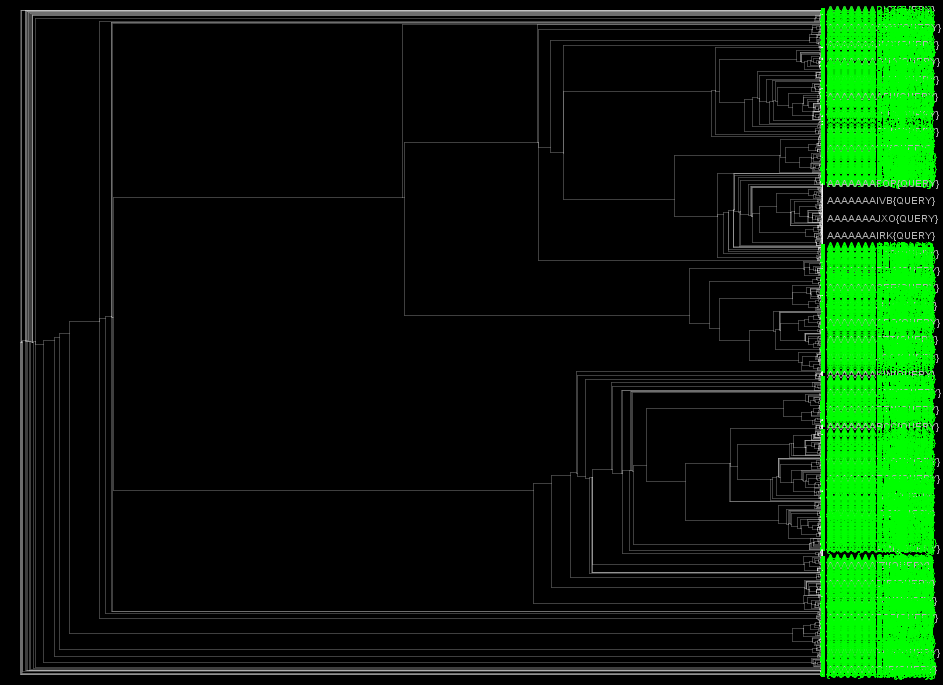
\includegraphics[width=.70\linewidth]{{upp/filtered}.png}\\
  \caption[]{Initial backbone sequences}
\end{subfigure}
\begin{subfigure}[htpb]{\textwidth}
  \centering
  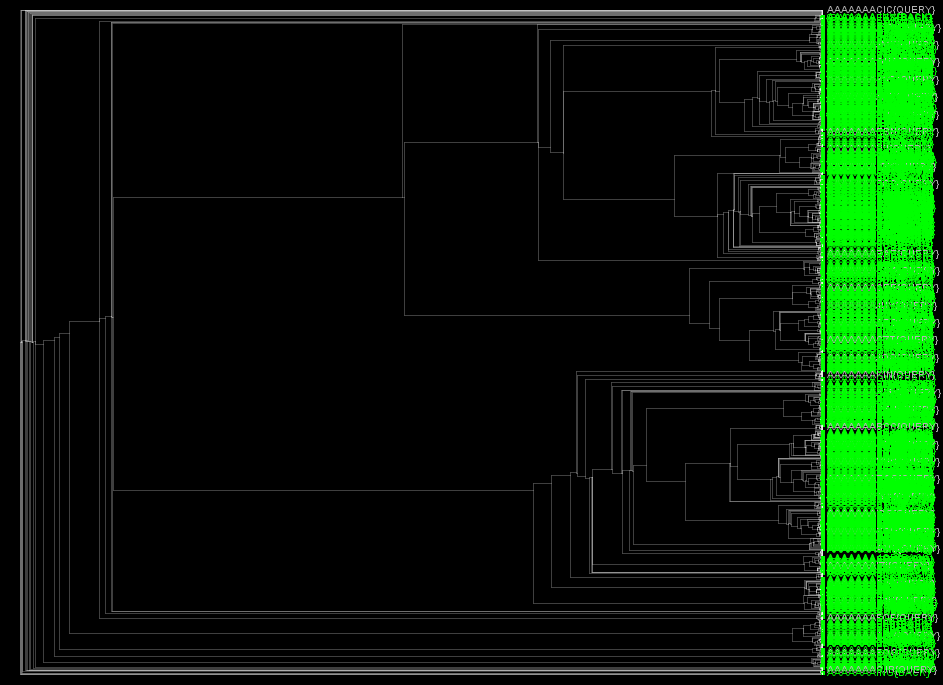
\includegraphics[width=.70\linewidth]{{upp/resampled}.png}\\
  \caption[]{Resampled backbone sequences}
\end{subfigure}
\caption[Distribution of the backbone sequences in the tree on the first
iteration of UPP on 16S.T.]{\label{resampling_figure}  {\bf Distribution of the backbone sequences in the estimated ML tree on 16S.T.}  We show the distribution of the backbone sequences (highlighted in green) in the ML tree estimated on the UPP(Default) alignment.  The initial selection of the backbone sequences resulted in sparse sampling throughout one clade.  After applying the resampling technique, the distribution of the backbone sequences show much more uniform coverage.}
\end{figure}

\clearpage
\subsection{Early termination on large datasets}\label{early_termination}
Many alignment methods failed to complete
analyses on the larger datasets,
but reasons varied. Some failed
due to insufficient memory, or due to a bug in the software, or 
were simply unable to produce an alignment within the 24 hour time limit 
(i.e., they might have been able to  produce an alignment if given more time).  
This section documents each case.  

\paragraph{MAFFT-default.}  MAFFT-default terminated early on the CRW 16S.B.ALL dataset due to the following error message:

\begin{verbatim} 
Cannot allocate 12568 character vector.
\end{verbatim}

MAFFT-default also failed to produce an alignment on the RNASim 100K dataset within the 24 hour time limit on TACC.  According MAFFT's output log, MAFFT was still running when the job was evicted.

\paragraph{MAFFT-PartTree.}  MAFFT-PartTree terminated with the following error message on the RNASim 200K dataset:

\begin{verbatim}
mafft: line 2028: 28963 Segmentation fault      
"$prefix/splittbfast" $legacygapopt -Z 
$algopt $splitopt $partorderopt $parttreeoutopt 
$memopt $seqtype $model -f "-"$gop -Q 
$spfactor -h $aof -p $partsize -s 
$groupsize $treealg -i infile > pre 2>> "$progressfile"
\end{verbatim}

\paragraph{MAFFT-addfragments.}  MAFFT ``addfragments'' terminated early on the RNASim datasets with 50,000 sequences or more, the CRW 16S.B.ALL dataset, and the HomFam aat, p450, rvp, and zf−CCHH datasets with the following error message (note that the line number and location of the segmentation fault was different for each dataset):

\begin{verbatim}
mafft: line XXXX: YYYYY Segmentation fault      
"$prefix/pairlocalalign" $localparam $addarg 
-C $numthreads $seqtype $model -g~$lexp 
-f~$lgop -Q~$spfactor -h $laof -Y 
< infile > /dev/null 2>> "$progressfile"
\end{verbatim}

\paragraph{MAFFT-add.}  MAFFT ``add'' terminated early on the Indelible 10000M2 dataset with the following error message: 

\begin{quote}
bug! hairetsu ga kowareta!
\end{quote}

On the RNASim 200K dataset, MAFFT ``add'' terminated with non-zero status, which signifies an error during execution.  

\paragraph{Opal.}  Opal failed to align the FastTree COG438 dataset, most likely due to a memory problem the machine.  The Opal log file shows that Opal terminated early during execution and that the peak virtual memory usage at the time was 31 GB (only 24 GB of RAM available on Lonestar machine).  

\paragraph{MUSCLE.} MUSCLE terminates early on the RNASim datasets with 50K sequences or more with the following error message:

\begin{verbatim}
*** OUT OF MEMORY *** 
Memory allocated so far 23718.4 MB 
No alignment generated
\end{verbatim}
On the HomFam zf-CCHH and rvp, MUSCLE terminated with the following error message: \emph{Segmentation fault}.

\paragraph{Clustal-Omega.}
Clustal-Omega failed to terminate within 24 hours on the RNASim datasets with 50,000 sequences or more.  The log file showed that Clustal-Omega was still running, so given enough time, it may be possible for Clustal-Omega to produce an alignment on the larger RNASim datasets.  

On the Indelible 10000M2 dataset, Clustal-Omega terminated early with the following error message:

\begin{verbatim}
HHalignWrapper:hhalign_wrapper.c:945: problem in 
alignment (profile sizes: 892 + 1540) (S1870 + S7661), 
forcing Viterbi
        hh-error-code=3 (mac-ram=2048)
+------------------------------+
| both sequences truncated right |
+------------------------------+
i2 = 2 != 6699 = qa->L, j2 = 10788 != 10846 = ta->L
PrintAlignments:hhhitlist-C.h:199: qt_ali.Build failed
hhalign:hhalign.cpp:1216: Could not print alignments
HHalignWrapper:hhalign_wrapper.c:984: 2nd attempt 
worked HHalignWrapper:hhalign_wrapper.c:945: 
problem in alignment
(profile sizes: 833 + 2432) (S3589 + S1870), forcing Viterbi
        hh-error-code=3 (mac-ram=2048)
\end{verbatim}

\clearpage

\section{Supplemental Figures and Tables}

\begin{table}[htpb]
\caption[Performance of UPP variants on the million-sequence RNASim dataset.]{\label{alignment_large}  
{\bf Results on the million-sequence RNASim dataset.}
We show results for UPP with a backbone of 100 sequences and using HMM families (labeled ``UPP(F)'') and using only a single HMM (labeled ``UPP(F,ND)'').
We also show results for UPP with a backbone of 1000 sequences
but without any decomposition (labeled  ``UPP(D,ND)''.  For
this dataset,  $\Delta{FN}$ is computed by comparing 
the difference in tree error between 
the estimated ML tree and the ML 
tree estimated on the masked true alignment (labeled ``TA''), where
any site with fewer than 1,000 ungapped characters was removed;
this masking was performed to reduce the size of the true alignment (21,946 before masking and 3,887 sites after masking) and make the ML tree estimation computationally feasible.  The tree error reported for the true alignment is also based on the masked true alignment.
The UPP alignments were computed on a dedicated
machine with 250 GB of memory and 12 CPUs; this is
a different computational platform than TACC's Lonestar Cluster machines, which we used to run the 
10K to 200K RNASim experiments, and so the running times
cannot be compared to results on the smaller RNASim datasets.}
   \centering
   \begin{tabular}{|r|r|l|l|l|r|}
   \hline
   Dataset & Method               & Align. Error &Tree error &$\Delta{FN}$& Time (hrs)\\
   %&&&& alignment time (hr) \\
   \hline
   1,000,000 & UPP(F,ND)    & 13.0\%       &   8.4\% & 2.8\%& 51.6                           \\
   1,000,000 & UPP(D,ND)        & 11.1\%     &    7.7\%&   2.1\%& 64.7                           \\
   \hline
   1,000,000 & UPP(F)        & 12.8\%     &   7.5\%  &  2.0\%& 286.4\\
   \hline   
   1,000,000 & TA        & 0.0\%     &   5.6\%  &  0.0\%& 0.0\\
   \hline   
   
   \end{tabular}
\end{table}

\begin{table}
    \caption[Empirical statistics for simulated datasets.]{\label{empirical_stats_simulated}  
{\bf Empirical statistics of the true alignments for the simulated datasets. }
The p-distance between two sequences is the proportion of fully ungapped sites in which they have different letters. 
Average p-distance is computed by averaging all p-distances between all pairs of sequences.  
Max p-distance is the maximum p-distance over all pairs of sequences.  
Values marked with an ``*'' were estimated by subsampling 1000 sequences at random and computing 
the empirical statistics of the sample.  
This was repeated 10 times, and the average of the results is
reported (with the 
exception of the max p-distance where we
report the maximum value of the replicates).}
    \scalebox{0.70}{
    \centering
    \begin{tabular}{lrrrrrrr}
    \hline
     Dataset & Number taxa& \# Sites ref. & Avg.~Seq.&Max& Avg.~seq. &Prop.~gapped& Avg.\\
    &&align&length &p-dist.&p-dist.&characters&gap length\\
    
    \hline
 1000L1           & 1,000  & 3,517                        &1,019.7      & 0.77            & 0.69           & 0.71           & 12.34          \\
 1000L2           & 1,000 & 2,830                            &   1,009.0& 0.77            & 0.70           & 0.64           & 13.15          \\
 1000L3           & 1,000 & 7,142                         &1,023.8      & 0.77            & 0.69           & 0.86           & 19.79          \\
 1000L4           & 1,000 & 2,249                         &1,007.9      & 0.61            & 0.51           & 0.55           & 10.07          \\
 1000L5           & 1,000       & 1,859                        &1,007.7 & 0.60            & 0.50           & 0.46           & 11.13          \\
 1000M1           & 1,000 & 3,880 &1012.9                         & 0.76            & 0.69           & 0.74           & 9.99           \\
 1000M2           & 1,000       & 4,068  &1,022.1                       & 0.77            & 0.69           & 0.75           & 10.35          \\
 1000M3           & 1,000       & 2,361         &1,006.2                & 0.75            & 0.66           & 0.57           & 6.90           \\
 1000M4           & 1,000       & 2,698 &1,008.2                        & 0.61            & 0.50           & 0.63           & 8.08           \\
 1000M5           & 1,000       & 1,690 &1,004.1                        & 0.61            & 0.50           & 0.41           & 5.77           \\
 1000S1           & 1,000       & 1,901   &1,004.5                      & 0.77            & 0.69           & 0.47           & 3.44           \\
 1000S2           & 1,000       & 1,441  &1,000.1                       & 0.76            & 0.69           & 0.31           & 2.61           \\
 1000S3           & 1,000       & 1,715  &1,001.4                       & 0.76            & 0.69           & 0.42           & 3.08           \\
 1000S4           & 1,000       & 1,288    &1,000.3                     & 0.61            & 0.50           & 0.22           & 2.38           \\
 1000S5           & 1,000       & 1,151    &999.9                     & 0.62            & 0.51           & 0.13           & 2.43           \\
\hline
 COG1028          & 5,000       & 251  &233.8                        & 0.92            & 0.62           & 0.07           & 3.05           \\
 COG1309          & 5,000       & 197   &179.4                       & 0.92            & 0.72           & 0.09           & 8.39           \\
 COG2814          & 5,000       & 384         &346.9                 & 1.00            & 0.65           & 0.10           & 12.57          \\
 COG438           & 5,000       & 380      &337.0                    & 0.88            & 0.68           & 0.11           & 7.64           \\
 COG583           & 5,000       & 296   &284.2                       & 1.00            & 0.67           & 0.04           & 2.95           \\
 COG596           & 5,000       & 281   &254.3                       & 1.00            & 0.71           & 0.09           & 5.93           \\
 COG642           & 5,000       & 322   &276.1                       & 0.89            & 0.65           & 0.14           & 12.22          \\
\hline
 10000M2          & 10,000      & 5,109&1,000.0                         & 0.75            & 0.68           & 0.80           & 6.83           \\
 10000M3          & 10,000      & 3,088 &1,000.3                        & 0.70            & 0.63           & 0.68           & 5.89           \\
 10000M4          & 10,000      & 1,831   &1,000.2                      & 0.59            & 0.51           & 0.45           & 5.10           \\
\hline
RNASim        10K            & 10,000      & 8,637  &1,554.6                       & 0.62            & 0.41           & 0.82           & 5.24\\
RNASim        50K            & 50,000      & 12,400        &1,554.6                 & 0.62            & 0.41           & 0.87           & 7.24\\    
RNASim        100K            & 100,000      & 14,316      &1,554.5                   & 0.61$^*$            & 0.41$^*$           & 0.89           & 8.41\\    
RNASim        200K            & 200,000      & 16,365      &1,554.5                   & 0.62$^*$            & 0.41$^*$           & 0.91           & 9.65\\
RNASim        1M            & 1,000,000      & 21,946    &1,554.5                     & 0.62$^*$            & 0.41$^*$           & 0.93           & 13.18$^*$\\    
    \hline
    \end{tabular}}
\end{table}

%    RNASim& 100000    & 100,000    & 14,316   & 0.891  & NA& NA                 \\
%    RNASim& 200000    & 200,000    & 16,365   & 0.905  & NA& NA                 \\


\begin{table}
    \caption[Empirical statistics for the biological datasets.]{\label{empirical_biological}  
{\bf Empirical statistics of the reference alignments of the biological datasets. }
The p-distance between two sequences is the proportion of fully ungapped sites in which they have different letters. Average p-distance is computed by averaging all p-distances between all pairs of sequences.  
Max p-distance is the maximum p-distance over all pairs of sequences.  
Some statistics for the HomFam datasets are computed only on the seed alignment;
thus the total number of taxa and average sequence length refer to the size and length of the HomFam seed sequences, and the total number of taxa and average sequence length of the entire HomFam dataset are shown in parentheses next to the seed size and seed length.}
    \scalebox{0.65}{
    \centering
    \begin{tabular}{lrrrrrrrr}
    \hline
      Dataset & Number & Sites in& Avg. Sequence&Max& Avg. &Prop.& Avg.\\
    &taxa &reference&length &p-distance&p-distance&gapped&gap\\
    &&alignment&&&&characters&length\\
\hline
 1GADBL\_100      & 561        & 490    &324.9                      & 0.71            & 0.46           & 0.34           & 7.04           \\
coli\_epi\_100   & 320        & 150      &133.1                    & 0.87            & 0.58           & 0.11           & 2.71           \\
RV100\_BBA0039   & 807        & 2,696          &395.1               & 1.00            & 0.42           & 0.85           & 57.41          \\
RV100\_BBA0067   & 410        & 1,092            &463.7             & 0.92            & 0.78           & 0.58           & 23.26          \\
RV100\_BBA0081   & 353        & 1,693                  &585.8       & 1.00            & 0.86           & 0.65           & 38.29          \\
RV100\_BBA0101   & 509        & 4,214                       &492.3  & 1.00            & 0.78           & 0.88           & 144.10         \\
RV100\_BBA0117   & 460        & 110   &56.7                       & 1.00            & 0.75           & 0.48           & 13.14          \\
RV100\_BBA0134   & 717        & 3,186      &470.2                   & 1.00            & 0.73           & 0.85           & 88.70          \\
RV100\_BBA0154   & 303        & 1,275            &518.5             & 0.85            & 0.66           & 0.59           & 28.46          \\
RV100\_BBA0190   & 397        & 2,547 &886.3                        & 1.00            & 0.69           & 0.65           & 26.57          \\
\hline
CRW        16S.3            & 6,323       & 8,716      &1557.2                   & 0.83            & 0.32           & 0.82           & 9.43           \\
CRW        16S.B.ALL        & 27,643      & 6,857             &1371.9            & 0.77            & 0.21           & 0.80           & 4.94           \\
CRW        16S.T            & 7,350       & 11,856    &1492.1                    & 0.90            & 0.34           & 0.87           & 12.09          \\
\hline
HomFam        aat              & 10 (25,100)         & 476              &403.6 (337.8)            & 0.87            & 0.71           & 0.15           & 4.09           \\
HomFam        Acetyltransf     & 6 (46,285)        & 229       &161.5 (83.0)                   & 0.87            & 0.75           & 0.29           & 6.98           \\
HomFam        adh              & 5 (21,331)         & 375   &373.6 (123.6)                       & 0.47            & 0.36           & 0.00           & 1.17           \\
HomFam        aldosered        & 7 (13,277)         & 386     &310.9 (268.6)                     & 0.79            & 0.57           & 0.19           & 5.11           \\
HomFam        biotin\_lipoyl   & 7 (11,833)         & 112     &83.4 (71.9)                     & 0.84            & 0.71           & 0.26           & 7.14           \\
HomFam        blmb             & 6 (17,200)         & 344     &241.7 (192.5)                     & 0.90            & 0.79           & 0.30           & 8.19           \\
HomFam        ghf13            & 10 (12,607)        & 626   &469.8 (264.5)                       & 0.84            & 0.72           & 0.25           & 5.06           \\
HomFam        gluts            & 14 (10,099)        & 235      &215.6 (98.1)                    & 0.81            & 0.60           & 0.08           & 3.08           \\
HomFam        hla              & 5 (13,465)         & 178    &178.0 (153.1)                      & 0.33            & 0.24           & 0.00           & 0.00           \\
HomFam        hom              & 8 (12,037)         & 98     &63.5 (53.5)                      & 0.84            & 0.64           & 0.35           & 9.52           \\
%HomFam        myb\_DNA-binding & 5 (10,398)         & 61     &53.6 (46.6)                      & 0.77            & 0.59           & 0.12           & 2.47           \\
HomFam        &&&&&&&\\
~~~myb\_DNA-binding & 5 (10,398)         & 61     &53.6 (46.6)                      & 0.77            & 0.59           & 0.12           & 2.47           \\
HomFam        p450             & 12 (21,013)        & 512     &408.0 (331.5)                     & 0.87            & 0.79           & 0.20           & 3.95           \\
HomFam        PDZ              & 6 (14,950)         & 110    &93.0 (80.9)                      & 0.84            & 0.69           & 0.15           & 3.19           \\
HomFam        Rhodanese        & 6 (14,049)         & 216    &150.0 (102.3)                      & 0.89            & 0.76           & 0.31           & 7.33           \\
%HomFam       & rhv              & 6          & 938                          & 0.77            & 0.66           & 0.17           & 7.20           \\
HomFam        rrm              & 20 (27,610)        & 157       &86.7 (67.5)                   & 0.91            & 0.77           & 0.45           & 8.28           \\
HomFam        rvp              & 6 (93,681)         & 132   & 106.33 (94.3)                       & 0.76            & 0.63           & 0.19           & 3.08           \\
HomFam        sdr              & 13 (50,157)        & 361   & 259.5 (163.3)                       & 0.89            & 0.77           & 0.28           & 4.70           \\
HomFam        tRNA-synt\_2b    & 5 (11,293)         & 467  & 307.8 (177.6)                        & 0.88            & 0.81           & 0.34           & 8.65           \\
HomFam        zf-CCHH          & 15 (88,345)        & 39   &29.1 (23.3)                        & 0.85            & 0.65           & 0.25           & 2.71           \\
    %Gutell & 16S.M     & 901    & 4,722  & 0.781 & 0.887& 0.3595\\
    %Gutell & 16S.M.aa\_ag     & 1,028    & 4,908  & 0.826 & 1.000& 0.342\\
%    Gutell & 16S.3     & 6,323    & 8,716  & 0.821 & 0.833& 0.315\\    
%    Gutell & 16S.T     & 7,350    & 11,856 & 0.874 & 0.901& 0.345\\
%    Gutell & 16S.B.ALL & 27,643   & 6,857  & 0.800 & 0.769 & 0.210\\
%    RNASim & 10000     & 10,000   & 8,637  & 0.820 & 0.616& 0.410\\
%    RNASim & 50000     & 50,000   & 12,400 & 0.875 & 0.621& 0.410  \\
%    RNASim& 100000    & 100,000    & 14,316   & 0.891  & NA& NA                 \\
%    RNASim& 200000    & 200,000    & 16,365   & 0.905  & NA& NA                 \\
    \hline
    \end{tabular}}
\end{table}
\clearpage
\subsection{Sequence length distribution}\label{length_distribution}
We display the sequence length distribution for the biological datasets in Figures~\ref{homfam_length}-\ref{balibase_length}.  The results show that there can be large sequence length heterogeneity within the protein family (e.g., ghf13 in Fig.~\ref{homfam_length} and RV100\_BBA0190 in Fig.~\ref{balibase_length}).

\begin{figure}[htpb]
\centering
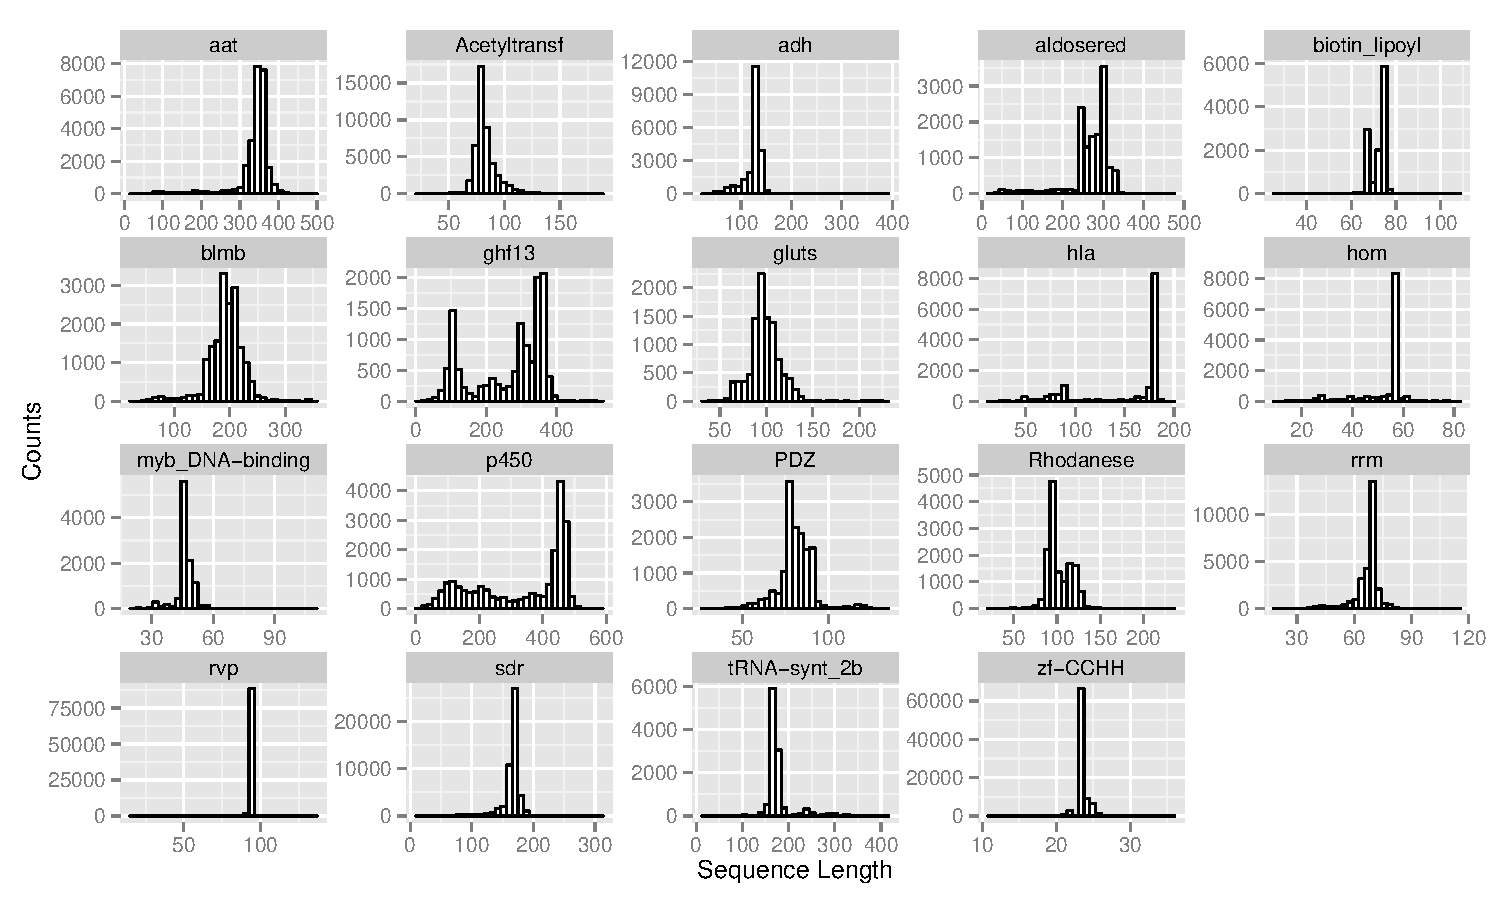
\includegraphics[width=1.1\linewidth]{{upp/length.homfam.1.30}.pdf}\\
\caption[Sequence length distributions of the HomFam datasets.]{\label{homfam_length}  
{\bf Sequence length distributions for the HomFam datasets.\textbf{NAM: Resize}}}
\end{figure}

\begin{figure}[htpb]
\centering
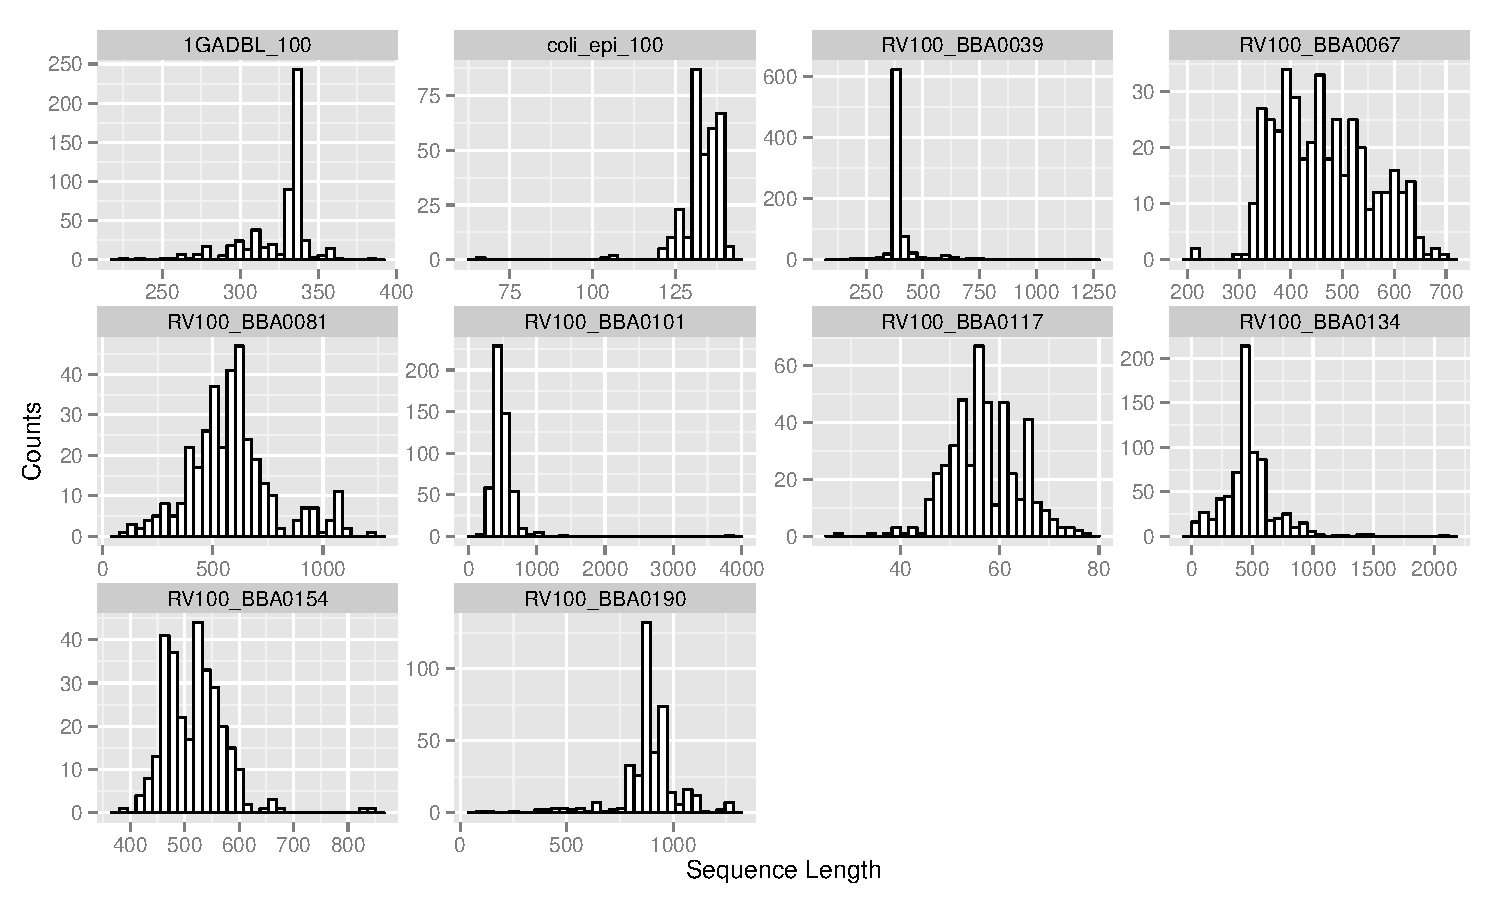
\includegraphics[width=1.1\linewidth]{{upp/length.balibase.1.30}.pdf}\\
\caption[Sequence length distributions of the ten large AA datasets.]{\label{balibase_length}  
{\bf Sequence length distributions for the ten large AA datasets 
with full reference alignments.\textbf{NAM: Resize}}}
\end{figure}

%Nam:  We didn't run the test on the HomFam because we never estimated trees on HomFam, we only focused on alignments.  
%Nam:  On balibase fragments were detected.  I didn't test on the large 10 AA. 

\clearpage
\subsection{Resampling on the CRW 16S.T dataset}\label{resample_16S}
The initial UPP alignment and tree on CRW 16S.T dataset triggered the resampling algorithm due to a sparse sampling of a major clade.
%described in Section~\ref{resampling}.  
A new backbone set was automatically selected using the resampling algorithm.  The new backbone set resulted in a more even sampling across the tree (Fig.~\ref{resampling_figure}).  Fig. \ref{gutell_iter_alignment} shows the alignment error for the first iteration (backbone set selected by random sampling of the full-length sequences) and the second iteration of UPP (uniform sampling across the ML tree).  While both iterations had very similar average alignment error 
(18.4\% for the first iteration and 18.2\% for the second iteration), 
the difference in $\Delta{FN}$ tree error was large (11.5\% 
for the first iteration and 6.6\% for the second).  
%Nam, what about $\Delta$FN?
%Closer inspection showed that the second iteration 
%recovered more homologies (SPFN error of 17.9\% and 14.4\% for 
%first and second iterations, respectively), though 
%at the cost of an increase in false homologies 
%(SPFP error of 18.7\% and 21.9\% for first and second iterations,
%respectively).  
%This result suggests that the 
%increased recovery of true homologies 
%outweighed the penalty for the increased estimation of false homologies.

\begin{figure}[htpb]
\begin{subfigure}[htpb]{\textwidth}
  \centering
  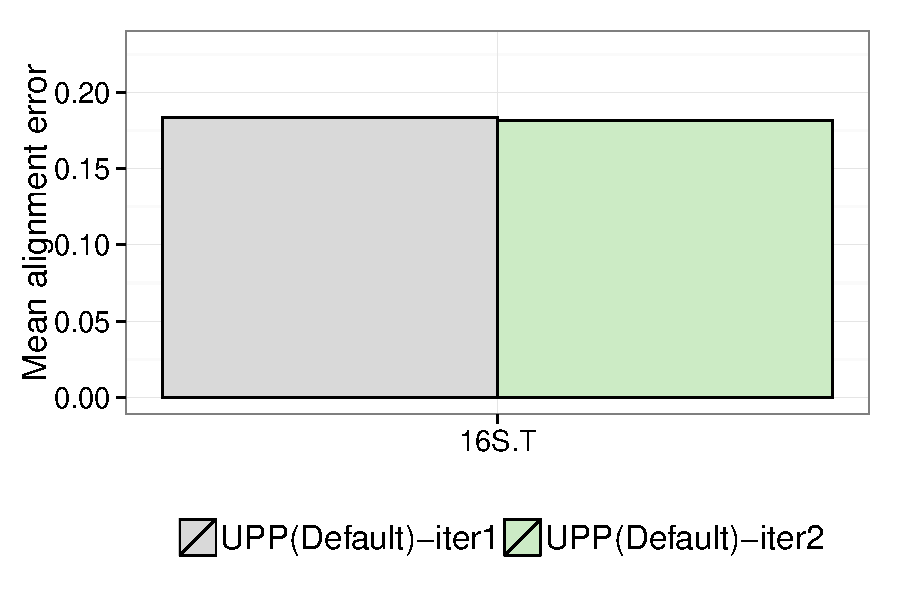
\includegraphics[width=0.50\linewidth]{{upp/gutell.iter.alignment_average}.pdf}\\
  \caption[]{Average alignment error}
\end{subfigure}
\begin{subfigure}[htpb]{\textwidth}
  \centering
  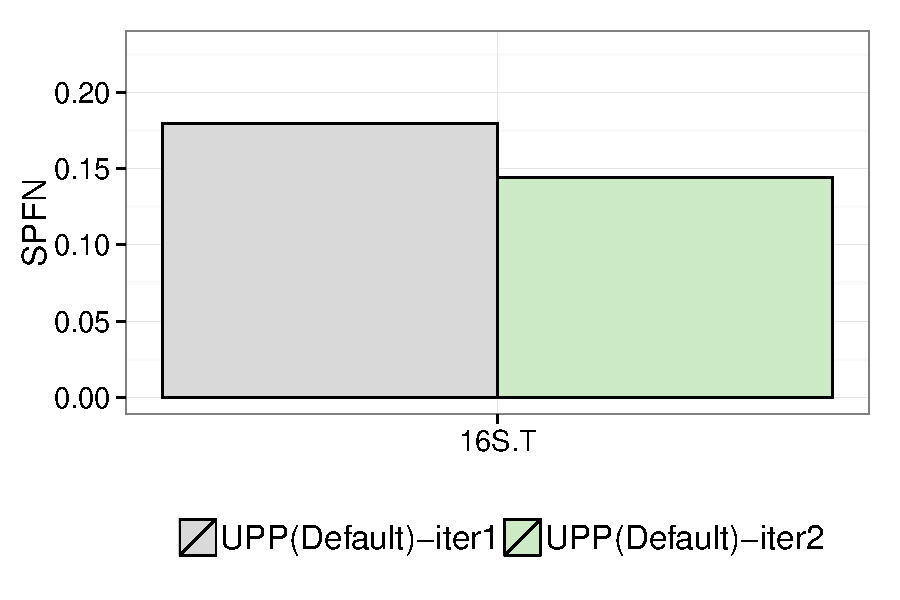
\includegraphics[width=0.50\linewidth]{{upp/gutell.iter.spfn}.pdf}\\
  \caption[]{Alignment SPFN error}
\end{subfigure}
\begin{subfigure}[htpb]{\textwidth}
  \centering
  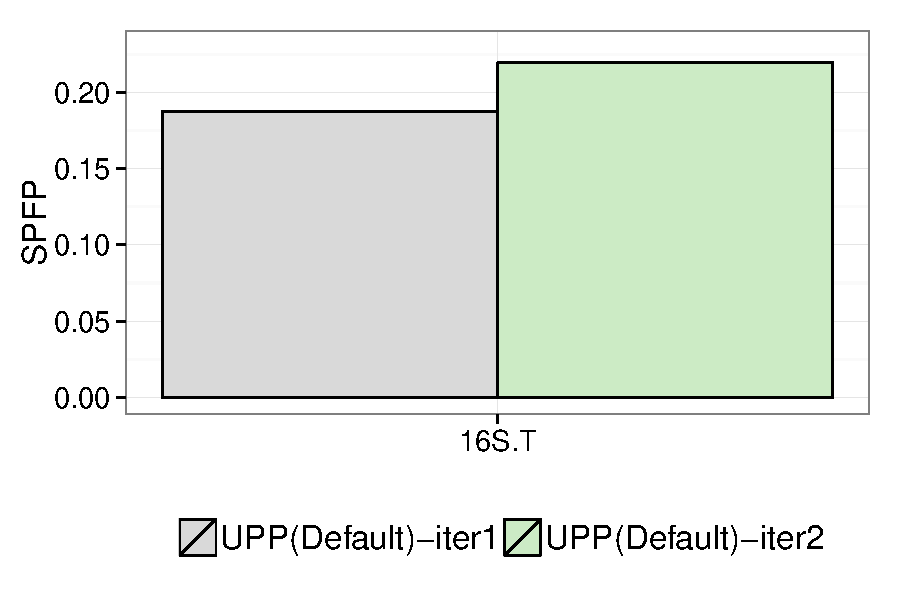
\includegraphics[width=0.50\linewidth]{{upp/gutell.iter.spfp}.pdf}\\
  \caption[]{Alignment SPFP error}
\end{subfigure}
\caption[Alignment error rates for the first two iterations of UPP on the CRW 16S.T dataset.]{\label{gutell_iter_alignment}  
{\bf Alignment error rates for the first two 
iterations of UPP on the CRW 16S.T dataset.}  The first iteration used a backbone sequence set selected by randomly sampling the full-length sequences from the dataset.  The resulting ML tree was scored with respect to the distribution of the backbone sequences throughout the tree and triggered a second iteration of UPP.  The second backbone was selected through the resampling algorithm.  We show results for the first and second UPP iterations.}  .
\end{figure}


\begin{figure}[htpb]
\begin{subfigure}[htpb]{\textwidth}
  \centering
  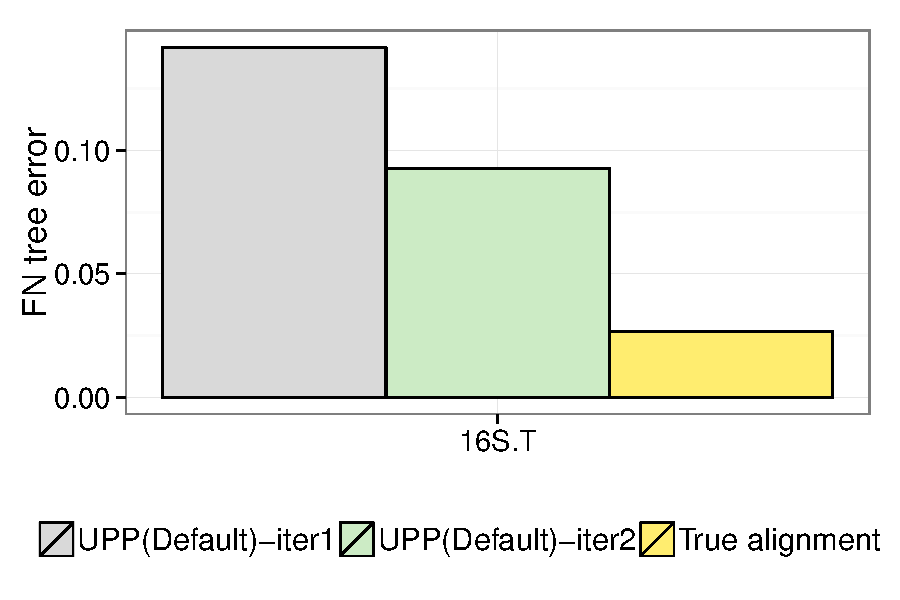
\includegraphics[width=0.70\linewidth]{{upp/gutell.iter.fn}.pdf}\\
  \caption[]{FN tree error} %\textbf{Need to figure out how to do multi-row legend in ggplot2}}
\end{subfigure}
\begin{subfigure}[htpb]{\textwidth}
  \centering
  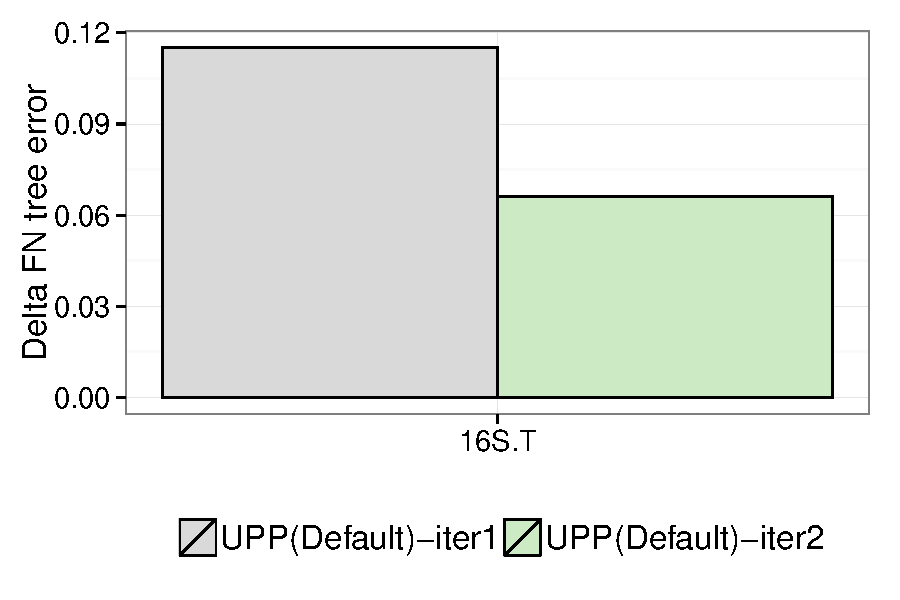
\includegraphics[width=0.70\linewidth]{{upp/gutell.iter.delta_fn}.pdf}\\
  \caption[]{Delta FN tree error }
\end{subfigure}
\caption[Tree error rates for first two iterations
of UPP on the CRW 16S.T dataset.]{\label{gutell_main_tree}{\bf  Tree error rates for 
first two iterations of UPP on the CRW 16S.T dataset.} 
The first iteration used a backbone sequence set selected by randomly sampling the full-length sequences from the dataset.  The resulting ML tree was scored with respect to the distribution of the backbone sequences throughout the ML tree and triggered a second iteration of UPP.  The second backbone was selected through the resampling algorithm.  We show results for the first and second UPP iterations.  ML trees were estimated using FastTree under GTR.}
\end{figure}
\clearpage

\subsection{UPP pipeline exploration\label{upp_variant}}
We examined different modifications to each stage of the UPP pipeline to examine the impact alignment and tree estimation accuracy.  We now give a brief overview and summary of our findings.

\clearpage
\subsubsection{Backbone alignment method}
We ran UPP(Fast) on the backbone alignments estimated using Clustal-Omega, MAFFT-L-INS-i, MUSCLE, and PASTA on backbone sets of size 100 on the RNASim 10K dataset (Fig.~\ref{rnasim_alignment_alignment} and \ref{rnasim_alignment_tree}.  We found that UPP using PASTA and MUSCLE backbones resulted in the most accurate UPP alignments, followed very closely by UPP on the MAFFT-L-INS-i backbone.  UPP on using the Clustal-Omega backbone, on the other hand, resulted in a distinctively worse alignment.  Curiously, while UPP on PASTA and MUSCLE backbones resulted in the best alignments, UPP on PASTA and MAFFT-L-INS alignments resulted in the best trees.  UPP on MUSCLE was close behind, and as before, UPP on Clustal-Omega was distinctly worse.  

%The finding that UPP on the PASTA backbone resulted in the lowest alignment error was not too surprising as the final UPP alignment error tends to closely match the initial backbone error (Fig.~\ref{backbone_error_alignment}; Section~\ref{backbone_alignment_error}).  

%Thus, since \cite{PASTA} showed that PASTA alignments were more accurate than other existing alignment methods on NT datasets under a wide range of conditions, we use PASTA to generate our backbone alignments.

%We ran UPP(Fast) on the backbone alignments estimated using Clustal-Omega, MAFFT-L-INS-i, MUSCLE, and PASTA alignments of size 100 on the RNASim 10K dataset (Fig.~\ref{rnasim_alignment_alignment} and \ref{rnasim_alignment_tree}.  We found that PASTA and MUSCLE backbones resulted in the most accurate alignments (13.3\% and 13.8\% alignment error), followed very closely by MAFFT-L-INS-i (14.9\%).  The Clustal-Omega backbone, on the other resulted in a distinctively worse alignment (23.2\%).  Curiously, while PASTA and MUSCLE backbones resulted in the best alignments, PASTA and MAFFT-L-INS alignments resulted in the best trees (11.8\% and 11.9\% FN error).  MUSCLE was close behind (12.1\%) and, as before, Clustal-Omega was distinctly worse (12.8\%).  The finding that the PASTA backbone resulted in the lowest alignment error was not too surprising as the final UPP alignment error tends to closely match the initial backbone error (Fig.~\ref{backbone_error_alignment}; Section~\ref{backbone_alignment_error}).  Thus, since \cite{PASTA} showed that PASTA alignments were more accurate than other existing alignment methods on NT datasets under a wide range of conditions, we use PASTA to generate our backbone alignments.


\begin{figure}[htpb]
\begin{subfigure}[htpb]{\textwidth}
  \centering
  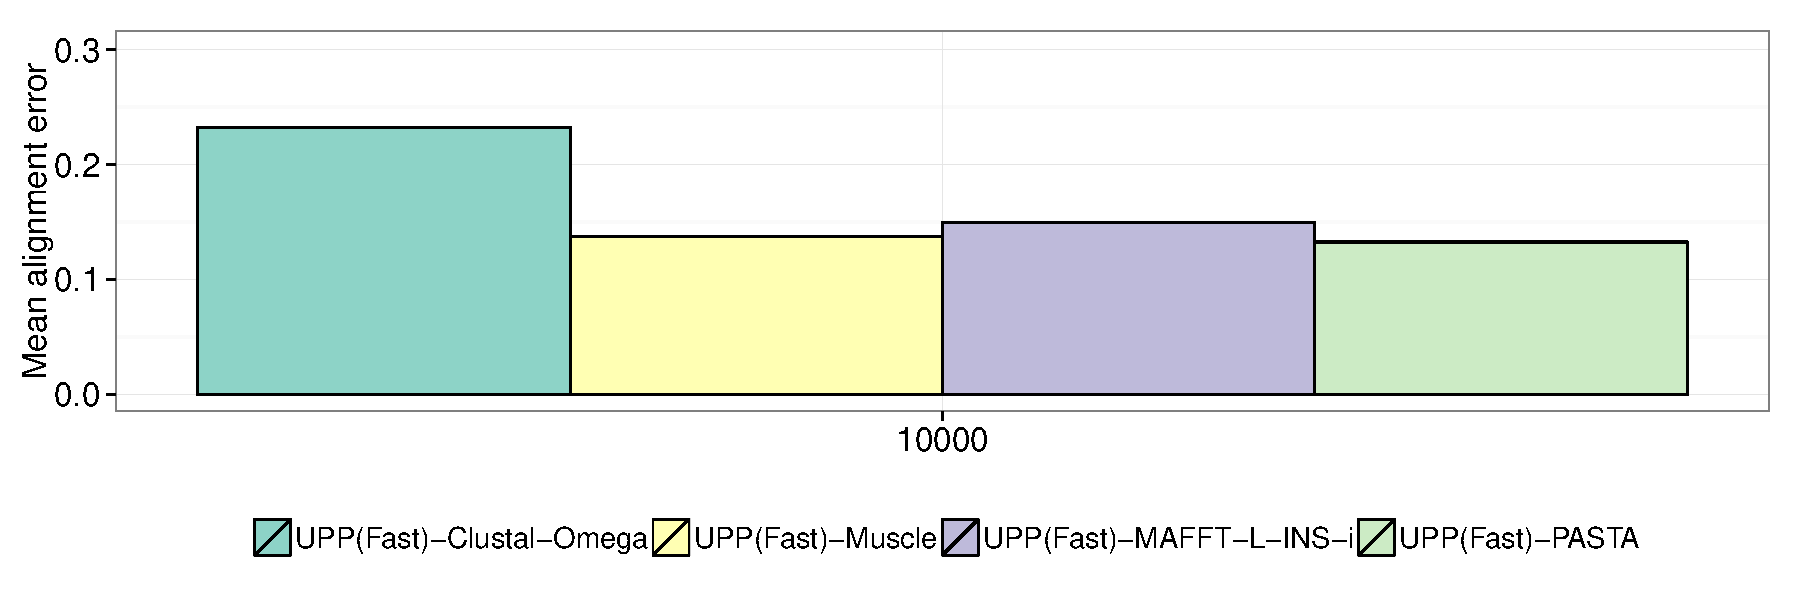
\includegraphics[width=0.9\linewidth]{{upp/rnasim.alignment.alignment_average}.pdf}\\
  \caption[]{Average alignment error}
\end{subfigure}
\begin{subfigure}[htpb]{\textwidth}
  \centering
  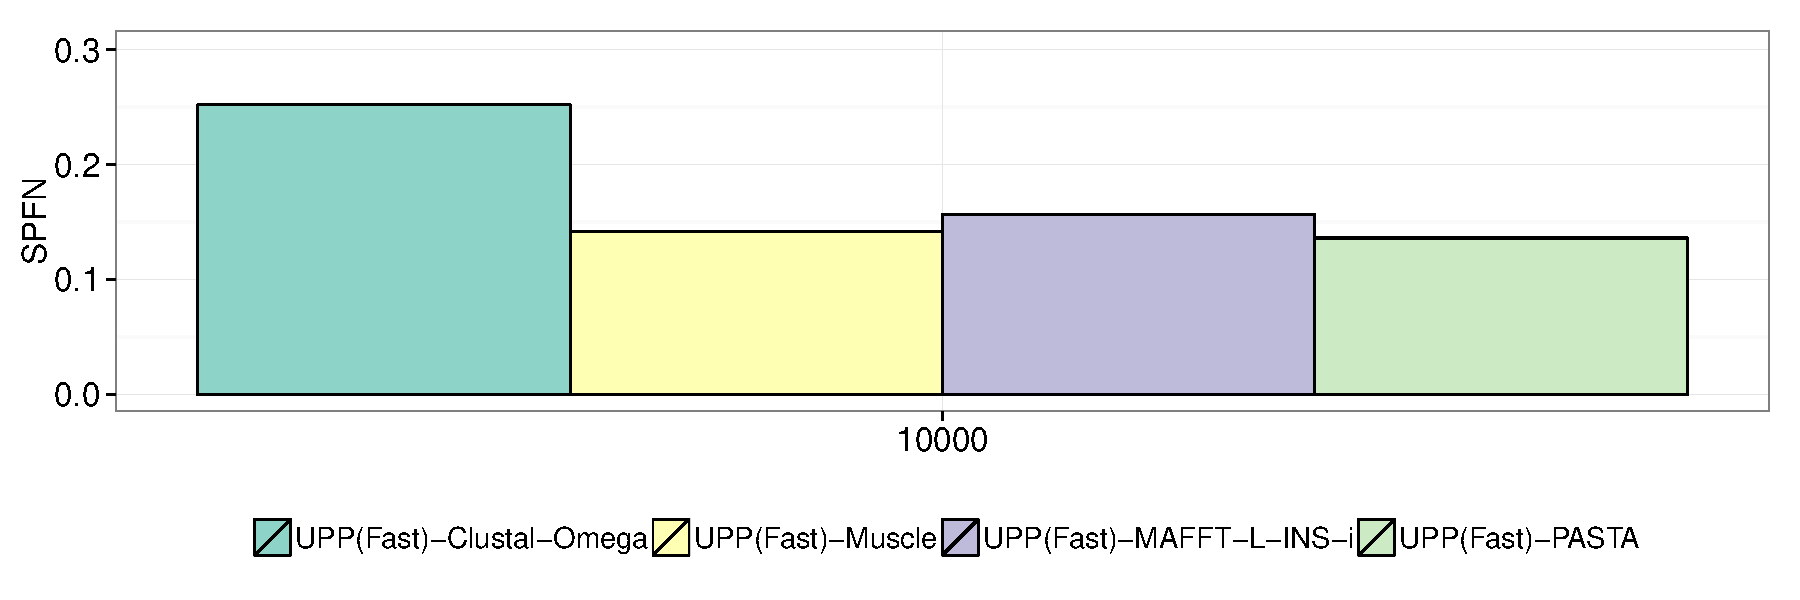
\includegraphics[width=0.9\linewidth]{{upp/rnasim.alignment.spfn}.pdf}\\
  \caption[]{Alignment SPFN error}
\end{subfigure}
\begin{subfigure}[htpb]{\textwidth}
  \centering
  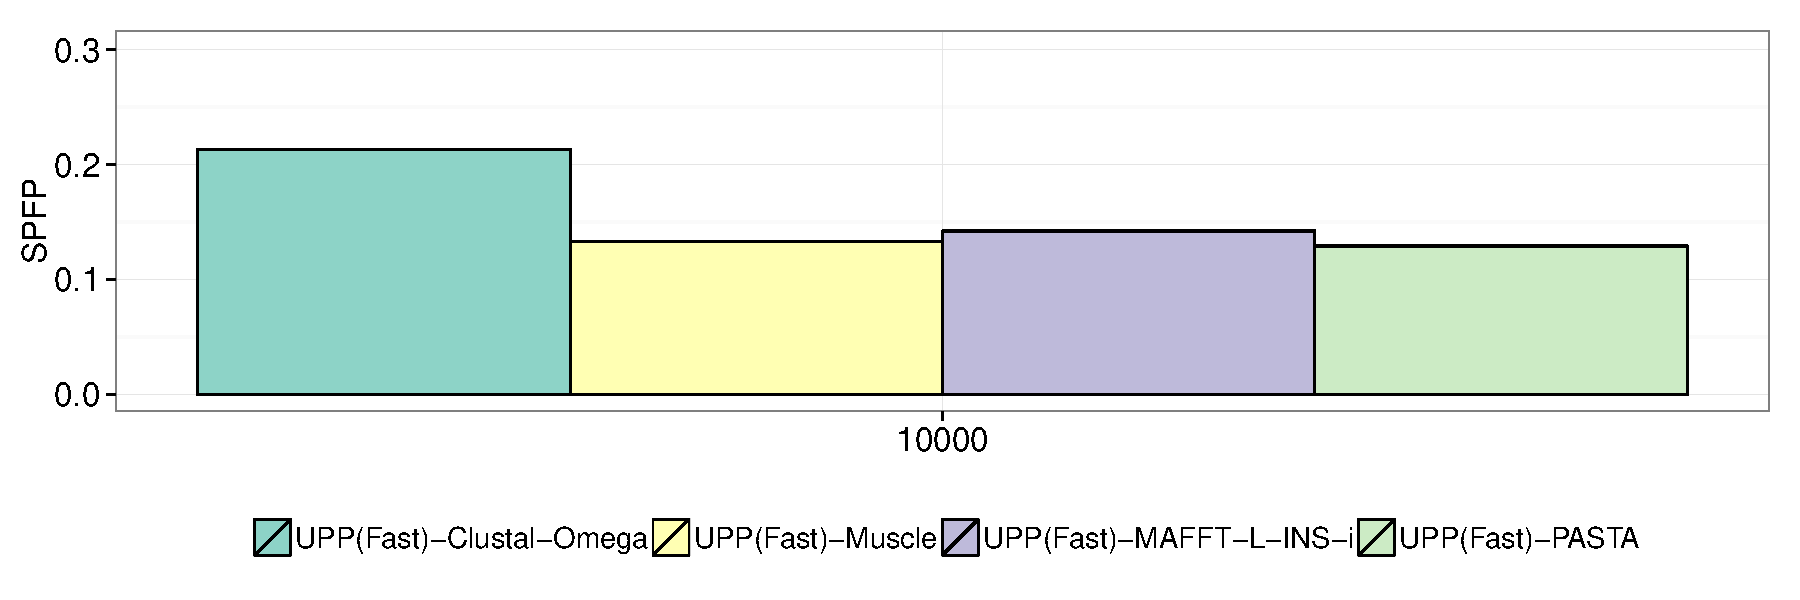
\includegraphics[width=0.9\linewidth]{{upp/rnasim.alignment.spfp}.pdf}\\
  \caption[]{Alignment SPFP error}
\end{subfigure}
\caption[Alignment error for different UPP backbone alignments on the RNASim 10K dataset.]{\label{rnasim_alignment_alignment}  {\bf Alignment
error rates of different UPP backbone alignments on the RNASim 10K dataset.}  All backbones are of size 100.\textbf{NAM: fix the x-axis text size}}
\end{figure}

\begin{figure}[htpb]
\begin{subfigure}[htpb]{\textwidth}
  \centering
  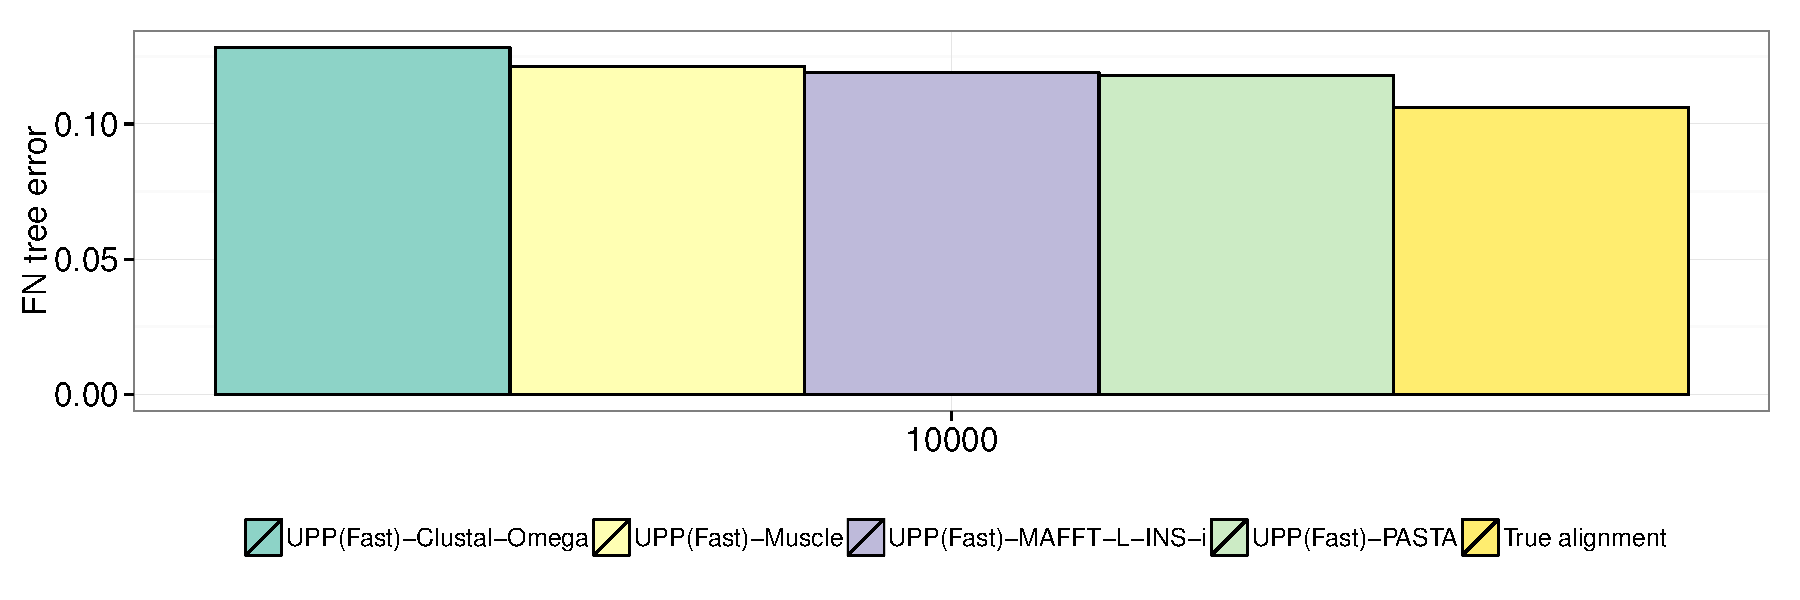
\includegraphics[width=0.90\linewidth]{{upp/rnasim.alignment.fn}.pdf}\\
  \caption[]{FN tree error}
\end{subfigure}
\begin{subfigure}[htpb]{\textwidth}
  \centering
  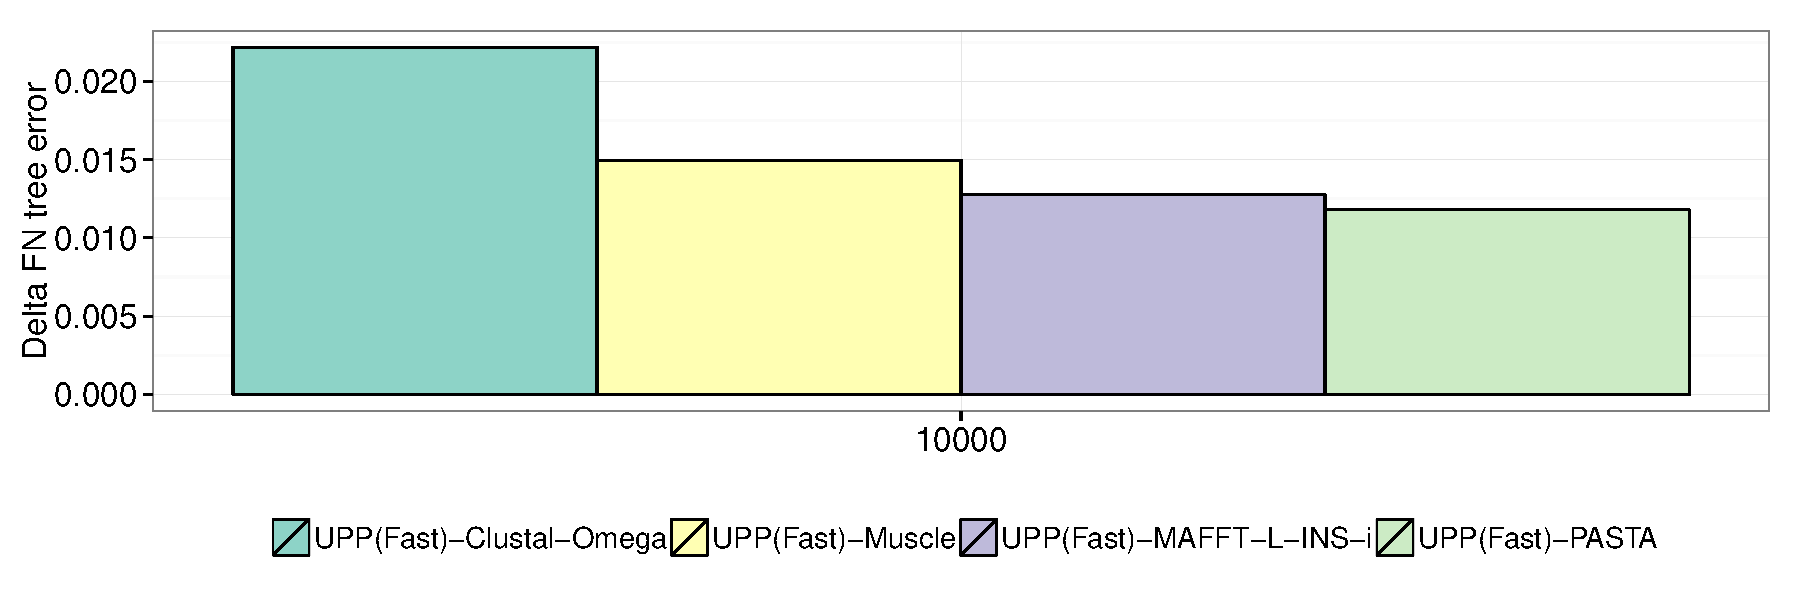
\includegraphics[width=0.90\linewidth]{{upp/rnasim.alignment.delta_fn}.pdf}\\
  \caption[]{Delta FN tree error}
\end{subfigure}
\caption[Tree error rates for different UPP backbone alignments on the RNASim 10K dataset.]{\label{rnasim_alignment_tree}  {\bf Tree error rates of different UPP backbone alignments on the RNASim 10K dataset.}  All backbones are of size 100.  ML trees were estimated using FastTree under GTR.}
\end{figure}

\clearpage 

\subsubsection{Backbone size}  
We examined the impact the backbone size on alignment and tree accuracy.  We compared the accuracy of UPP using the HMM Family technique (or a single HMM) with UPP using
MAFFT-Profile on small (100) and large (1000) backbones.  We denote methods that used the small backbone as ``Fast'' and methods that used the large backbone as ``Default''.  

In general, using a larger backbone resulted in more accurate alignments and trees for both UPP and MAFFT-Profile-add (Fig.~\ref{rnasim_backbone}).  
\clearpage
\subsubsection{Query sequence alignment method.}  

We compared three different technique for aligning 
the query sequences to the backbone alignment within the UPP pipeline: using the HMM Family
technique, using 
MAFFT-Profile ``-{}-add'', and using MAFFT-Profile ``-{}-addfragments''. 
Figure \ref{rnasim_backbone} showed that the HMM Family technique  
resulted in more accurate alignments and trees than MAFFT-Profile,
whether using -{}-add or -{}-addfragments.   
In addition, UPP using the HMM Family technique made it possible to align 
200,000 sequences within 24 hours, but UPP using   MAFFT-Profile ``-{}-add'' 
was  unable to align the 200K dataset in that timeframe, and UPP using
 MAFFT-Profile ``-{}-addfragments'' could only align up to 10,000 sequences (Table 1 from main document).  Comparing MAFFT-Profile ``-{}-add'' and MAFFT-Profile ``-{}-addfragments'', we found that MAFFT-Profile ``-{}-addfragments'' resulted in more accurate alignments and trees than MAFFT-add~ (Fig. \ref{rnasim_backbone}), at a large increase in running time (Table 1 from main document), however, neither MAFFT variants were as accurate as the HMM Family technique.

% (for results comparing variants of UPP, see next paragraph).  

%We start with a comparison between MAFFT-Profile within UPP, and so we also explore variants of MAFFT-Profile, focusing closely on the comparison between MAFFT-Profile using local alignment (``-~-addfragments'' option) versus global alignment (``-~-add'' option).  We found that MAFFT-Profile-AddFragments was more robust (MAFFT-Profile ``-~-add'' failed to align the 10000M2 dataset due to a bug and also oftentimes failed to align the Gutell 16S.B.ALL fragmentary datasets).  As expected, MAFFT-Profile with ``-~-addfragments'' had better alignments and trees on the simulated fragmentary datasets (Figs~\ref{} \textbf{Nam: we only had mafft addfragment results for 1000-taxa using new protocol for selecting backbone, previous results for fragmentary sequences comparing mafft-add versus addfragments were older results on backbone of size 100 instead of new protocol; I'll run add on under new protocol once lonstar is up again, but if trends hold, addfragments will be much more accurate.  March 8}).  More surprisingly was that MAFFT-Profile ``-~-addfragments'' can vastly outperform MAFFT-Profile ``-~-add'' on full-length sequences (Figs~\ref{indelible_mafft_frag_alignment} and \ref{indelible_mafft_frag_tree} and Table~\ref{upp_rnasim}), though MAFFT-Profile ``-{}-addfragments'' was more computationally expensive to run.

\begin{figure}[htpb]
\begin{subfigure}[htpb]{\textwidth}
  \centering
  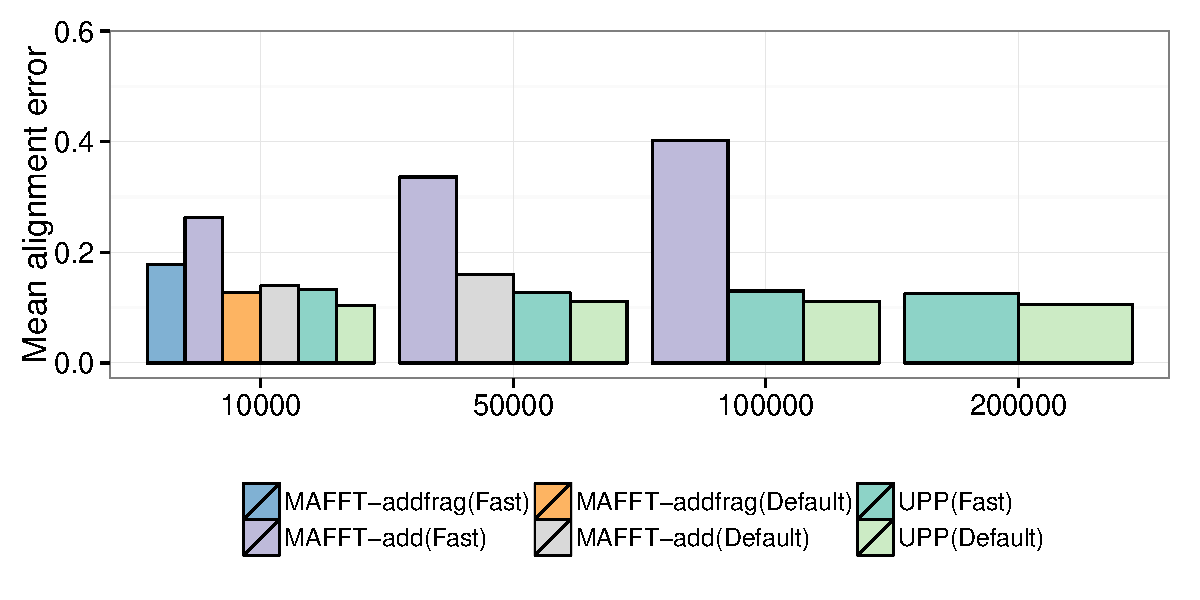
\includegraphics[width=.90\linewidth]{{upp/rnasim.backbone_size.alignment_average}.pdf}\\
  \caption[]{Average alignment error}
\end{subfigure}
\begin{subfigure}[htpb]{\textwidth}
  \centering
  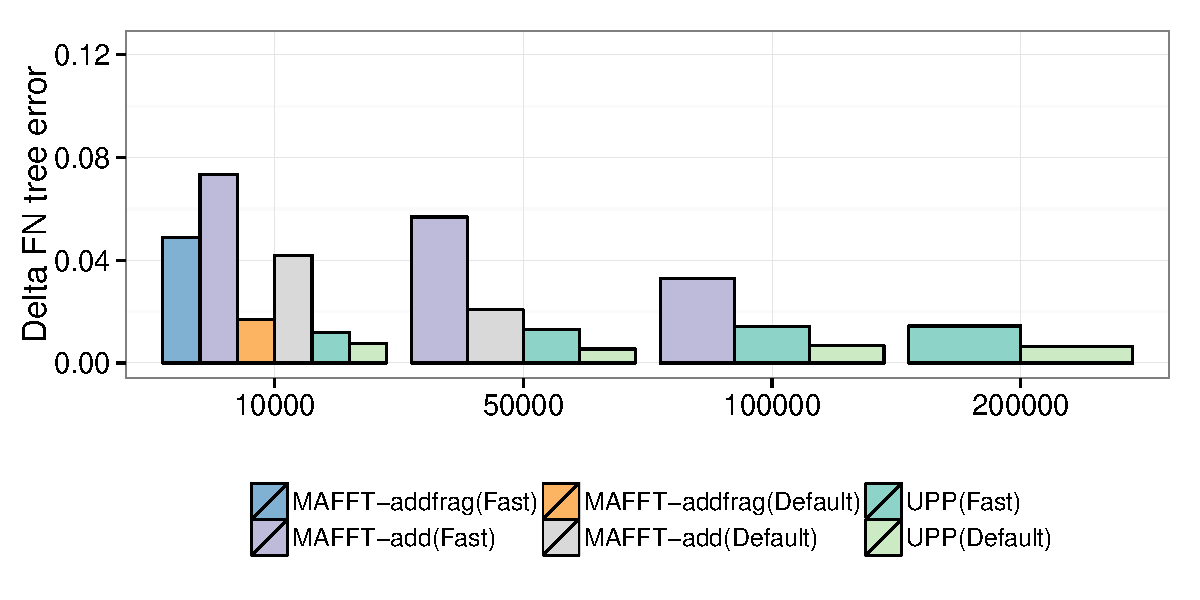
\includegraphics[width=.90\linewidth]{{upp/rnasim.backbone_size.delta_fn}.pdf}\\
  \caption[]{Delta tree error}
\end{subfigure}
\caption[Alignment and tree error of UPP variants on %for small and large backbones on 
the RNASim datasets.]{\label{rnasim_backbone}  {\bf Alignment and tree error for 
UPP variants on  the RNASim datasets.}  Methods labeled with ``Default'' use a backbone size of 1000.  Methods labeled with ``Fast'' use a backbone size of 100.  ML trees were estimated using FastTree under GTR.}
\end{figure}

%In general, using a larger backbone resulted in more accurate alignments and more accurate trees for both UPP (UPP(Default) has 10.6\% alignment error and 0.7\% $\Delta{FN}$ tree error compared to 12.5\% alignment error and for UPP(Fast) 1.4\% $\Delta{FN}$ tree error on RNASim 200K; Fig.~\ref{rnasim_backbone}) and MAFFT-Profile-add (MAFFT-add(Default) has 16.0\% alignment error and 2.1\% $\Delta{FN}$ tree error compared to MAFFT-add(Fast) has 33.6\% alignment error and 5.7\% $\Delta{FN}$ tree error on RNASim 50K; Fig.~\ref{rnasim_backbone}).  The improved accuracy comes at the cost of increased running time (UPP(Fast) required 17.9 hours compared to 151 hours ) hours for UPP(Default) on the RNASim 200K dataset.

\clearpage
\subsubsection{Impact of using the HMM Family technique or a single HMM}  
We explored in more detail the impact of using a single HMM to represent the backbone alignment (UPP with no decomposition) versus using the family of HMMs (UPP with decomposition) on both small (100) and large (1000) backbone sizes.  In general, there are very minor differences between using a single HMM and the family of HMMs with respect to alignment error (Figs.~\ref{rnasim_upp_alignment} and ~\ref{gutell_upp_alignment}).  There are exceptions, however.  The CRW 16S.T dataset cannot be fully aligned using a single HMM.  The dataset contains a sequence which HMMALIGN cannot align to the HMM computed on the entire backbone for both ``Fast'' and ``Default''  versions of the backbones.  However, when decomposition is applied, every sequence in 16S.T can be aligned.  Thus, the family of HMMs technique is essential for generating an alignment on some datasets.

The impact of decomposition is much more substantial with respect to tree accuracy: UPP with decomposition resulted in significantly more accurate trees (Fig.~\ref{rnasim_upp_tree} and ~\ref{gutell_upp_tree}). However, decomposition does come with a significant increase in running time (Fig.~\ref{rnasim_upp_time}).


\begin{figure}[htpb]
\begin{subfigure}[htpb]{\textwidth}
  \centering
  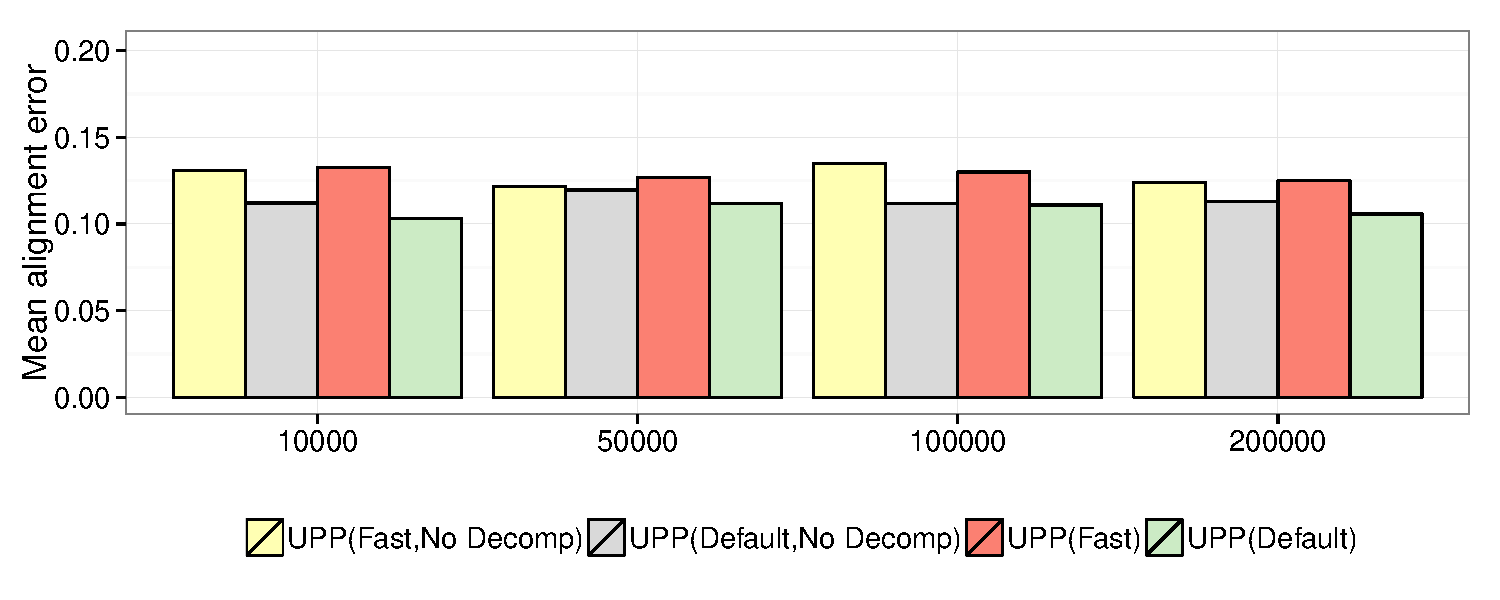
\includegraphics[width=0.80\linewidth]{{upp/rnasim.upp.alignment_average}.pdf}\\
  \caption[]{Average alignment error}
\end{subfigure}
\begin{subfigure}[htpb]{\textwidth}
  \centering
  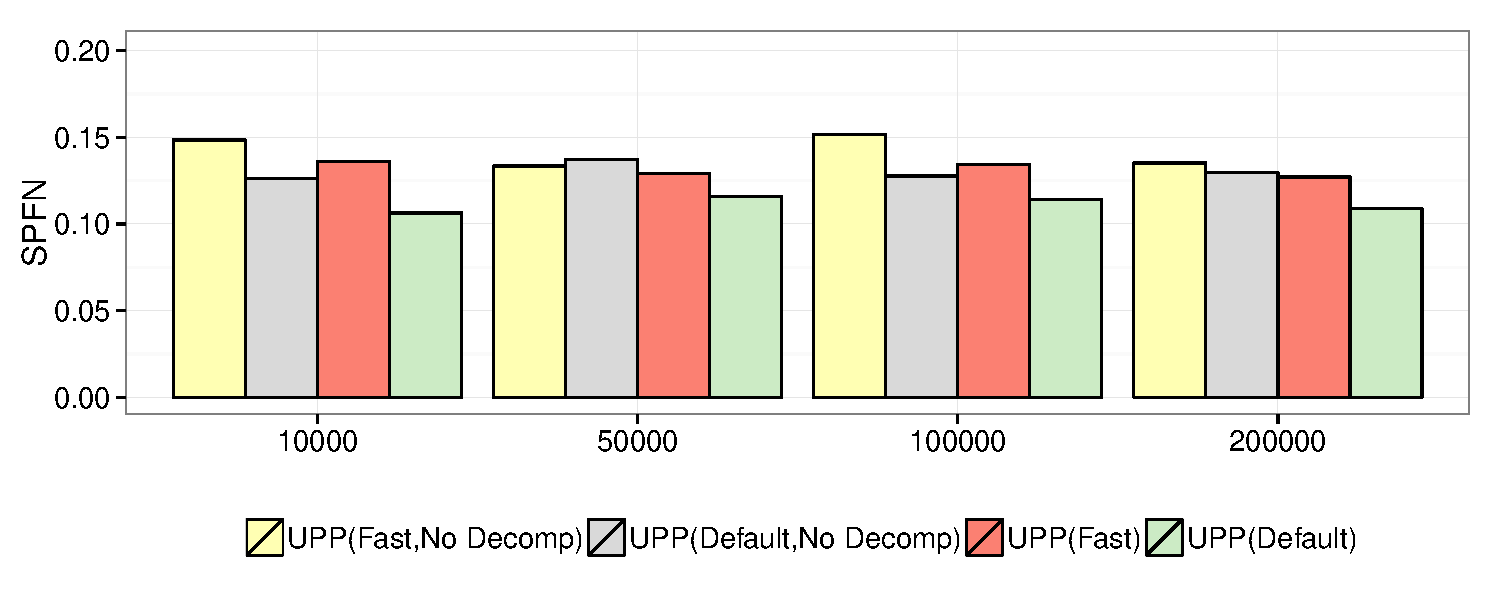
\includegraphics[width=0.80\linewidth]{{upp/rnasim.upp.spfn}.pdf}\\
  \caption[]{Alignment SPFN error}
\end{subfigure}
\begin{subfigure}[htpb]{\textwidth}
  \centering
  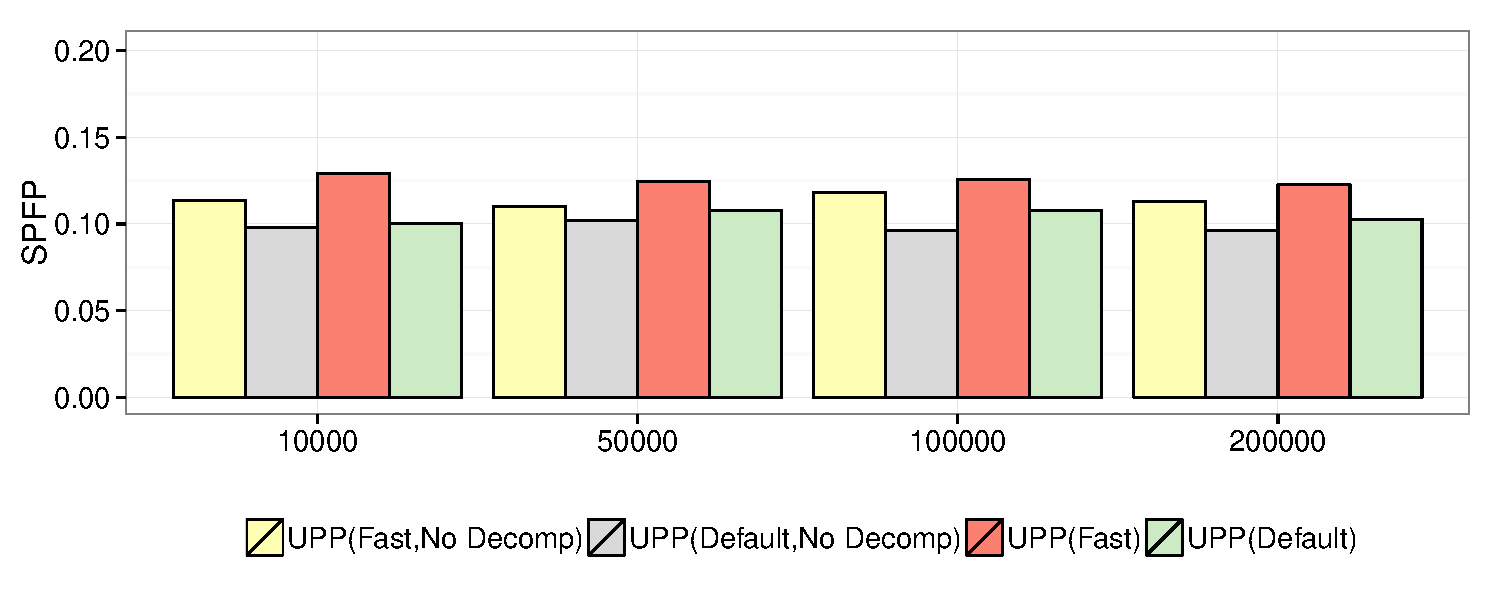
\includegraphics[width=0.80\linewidth]{{upp/rnasim.upp.spfp}.pdf}\\
  \caption[]{Alignment SPFP error}
\end{subfigure}
\caption[Alignment error of UPP variants on
the RNASim datasets.]{\label{rnasim_upp_alignment}  {\bf Alignment
error for UPP variants on the RNASim datasets.}  Methods labeled with ``Default'' use a backbone size of 1000.  Methods labeled with ``Fast'' use a backbone size of 100.}
\end{figure}

\begin{figure}[htpb]
\begin{subfigure}[htpb]{\textwidth}
  \centering
  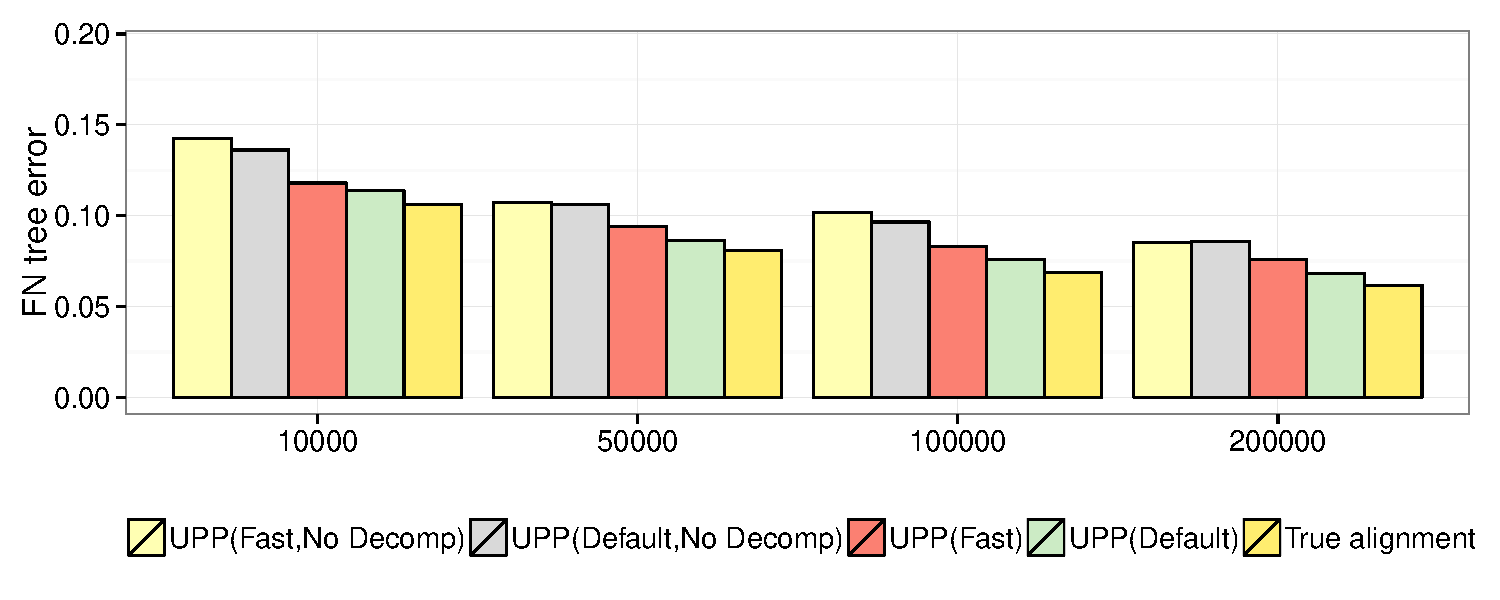
\includegraphics[width=0.90\linewidth]{{upp/rnasim.upp.fn}.pdf}\\
  \caption[]{FN tree error}
\end{subfigure}
\begin{subfigure}[htpb]{\textwidth}
  \centering
  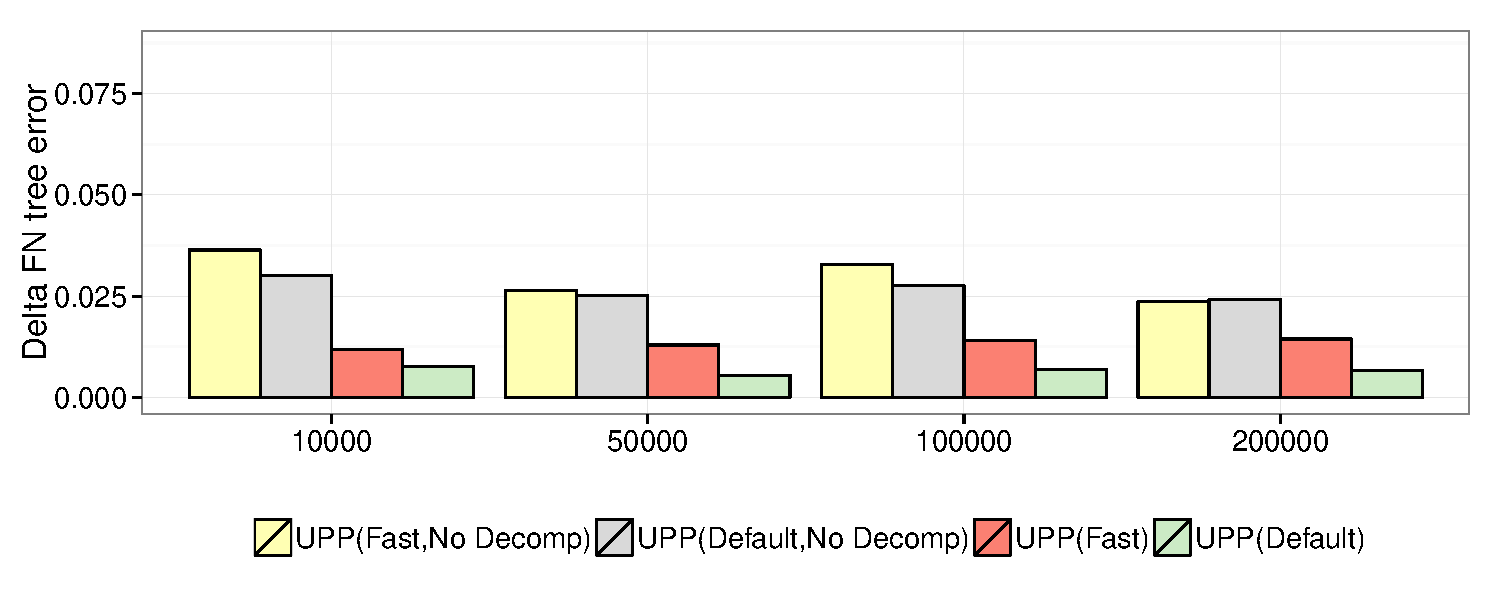
\includegraphics[width=0.90\linewidth]{{upp/rnasim.upp.delta_fn}.pdf}\\
  \caption[]{Delta FN tree error}
\end{subfigure}
\caption[Tree error of UPP variants for  
RNASim datasets.]{\label{rnasim_upp_tree}  {\bf Tree error of UPP variants on the RNASim datasets.}  Methods labeled with ``Default'' use a backbone size of 1000.  Methods labeled with ``Fast'' use a backbone size of 100.  ML trees were estimated using FastTree under GTR.}
\end{figure}

\begin{figure}[htpb]
\centering
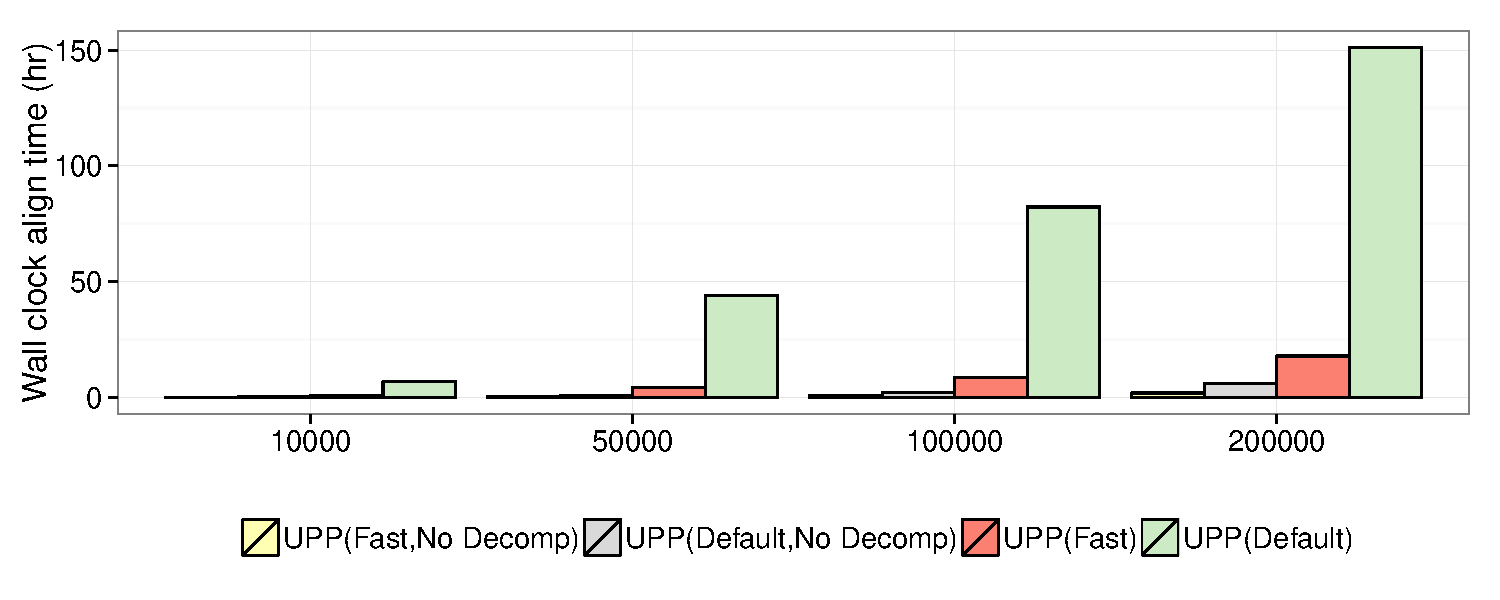
\includegraphics[width=1.0\linewidth]{{upp/rnasim.upp.wall_align_time}.pdf}\\
\caption[Wall clock alignment time (hrs) of UPP variants on the
RNASim datasets.]{\label{rnasim_upp_time}  {\bf  Wall clock alignment time (hrs) of UPP variants on the RNASim datasets.}  
All methods were run on a machine with 12 CPUs and 24 GB of memory.  Methods labeled with ``Default'' use a backbone size of 1000.  Methods labeled with ``Fast'' use a backbone size of 100.  ML trees were estimated using FastTree under GTR.}
\end{figure}

\begin{figure}[htpb]
\begin{subfigure}[htpb]{\textwidth}
  \centering
  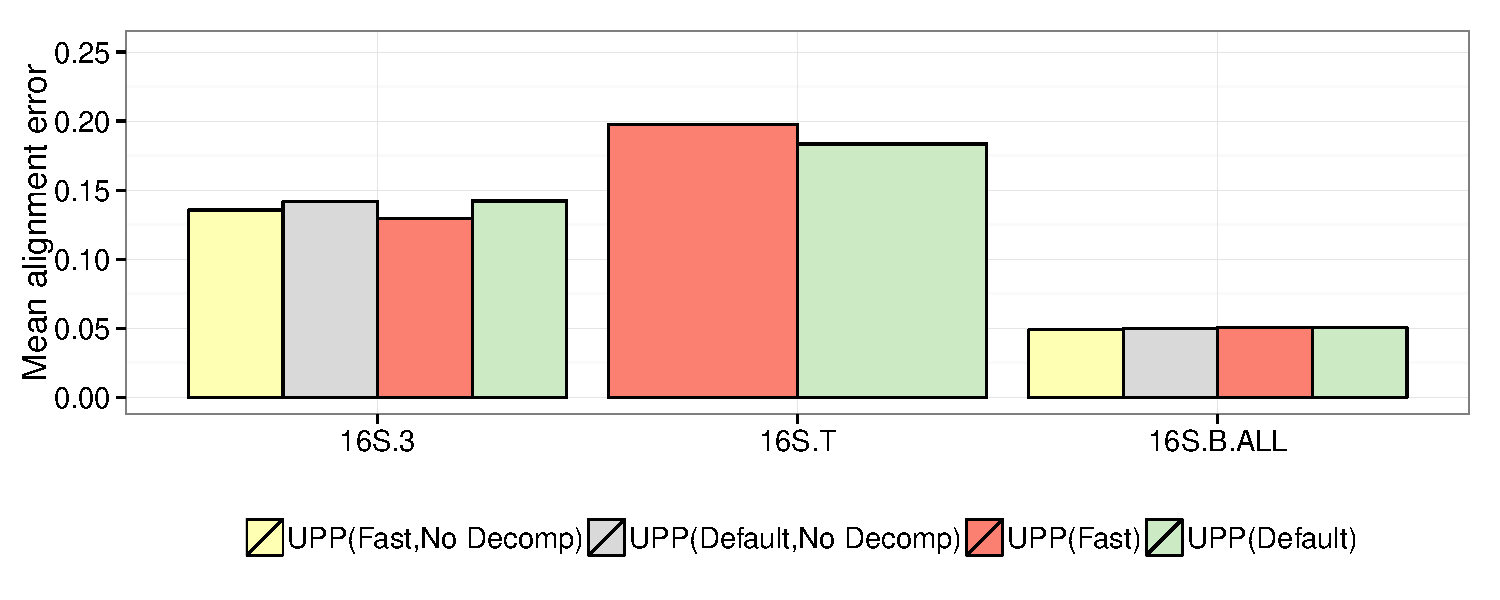
\includegraphics[width=0.70\linewidth]{{upp/gutell.upp.alignment_average}.pdf}\\
  \caption[]{Average alignment error}
\end{subfigure}
\begin{subfigure}[htpb]{\textwidth}
  \centering
  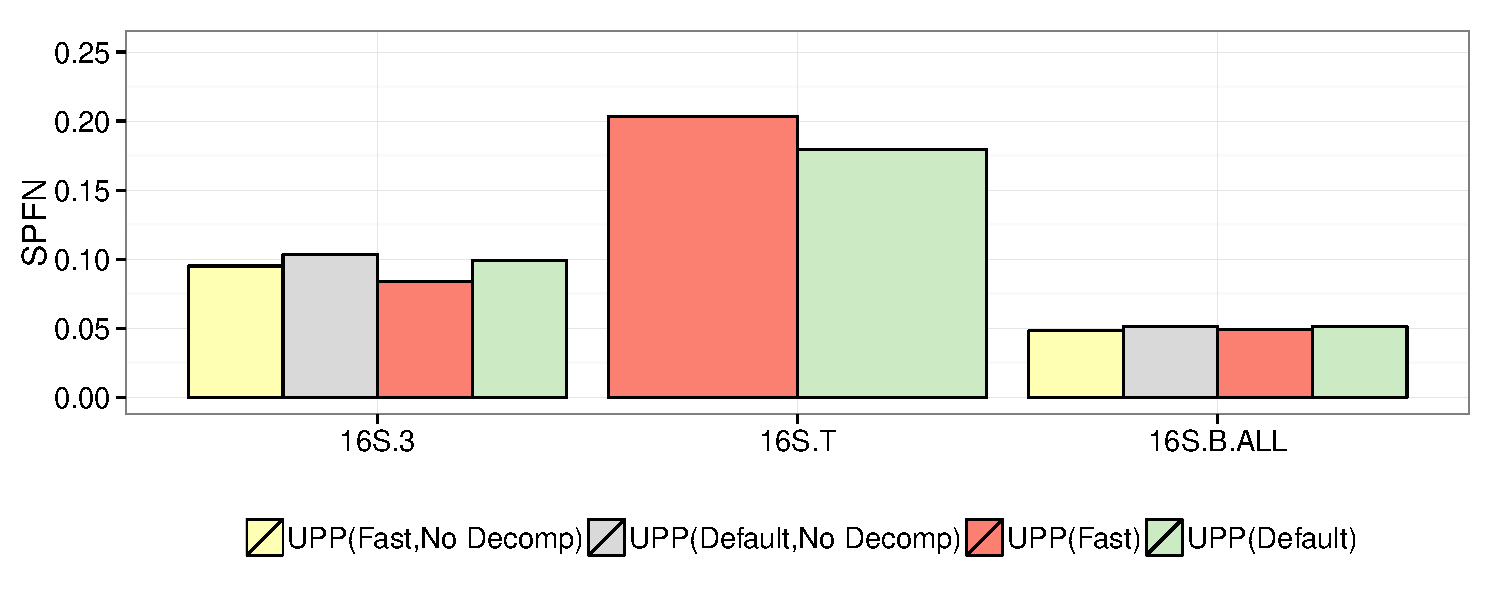
\includegraphics[width=0.70\linewidth]{{upp/gutell.upp.spfn}.pdf}\\
  \caption[]{Alignment SPFN error}
\end{subfigure}
\begin{subfigure}[htpb]{\textwidth}
  \centering
  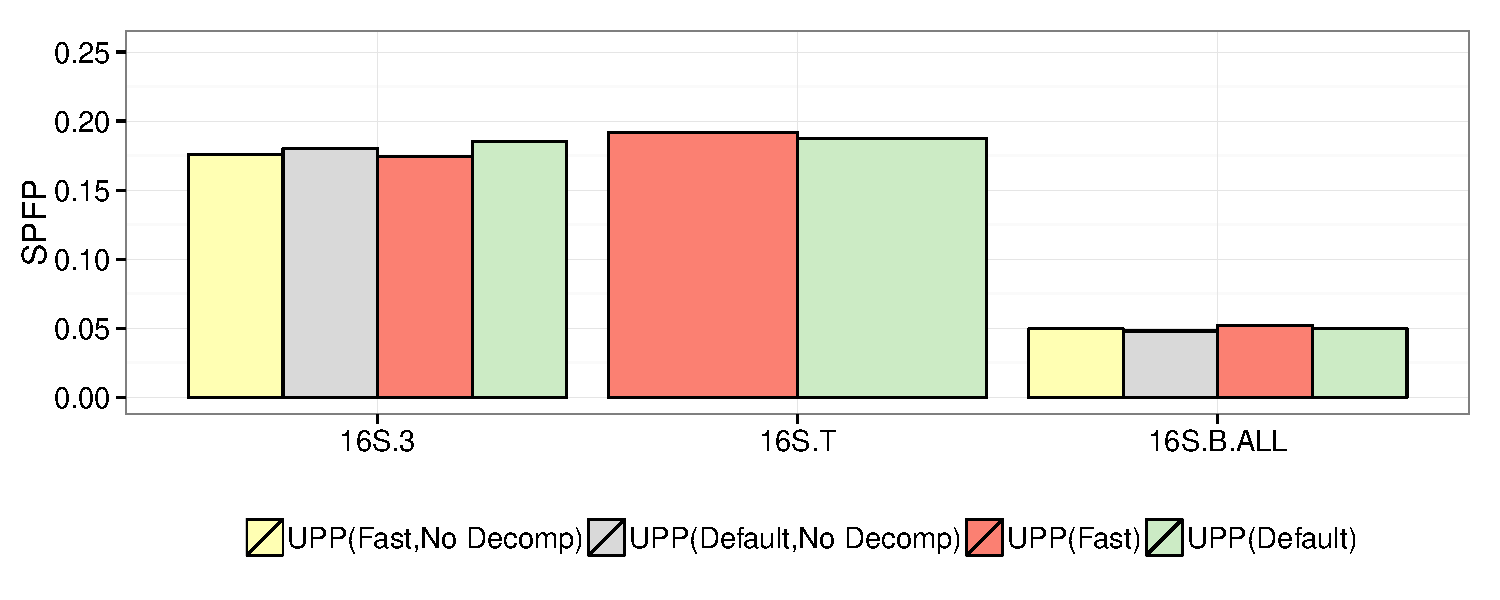
\includegraphics[width=0.70\linewidth]{{upp/gutell.upp.spfp}.pdf}\\
  \caption[]{Alignment SPFP error}
\end{subfigure}
\caption[Alignment error of UPP variants on the
CRW 16S datasets.]{\label{gutell_upp_alignment}  {\bf Alignment
error for UPP variants on the CRW 16S datasets.}  Methods labeled with ``Default'' use a backbone size of 1000.  Methods labeled with ``Fast'' use a backbone size of 100.  Both UPP(Default,No Decomp) and UPP(Fast,No Decomp) failed to align one of the 16S.T sequences and thus failed to generate an alignment on the entire dataset.  UPP results are based on the first iteration of UPP.}
\end{figure}
%Nam - is this two iterations or one?
%One iteration, we didn't have time to iterate on all the 16S.T variants, i.e., we would also need to iterate on UPP(Fast) if we plan to apply it everywhere

\begin{figure}[htpb]
\begin{subfigure}[htpb]{\textwidth}
  \centering
  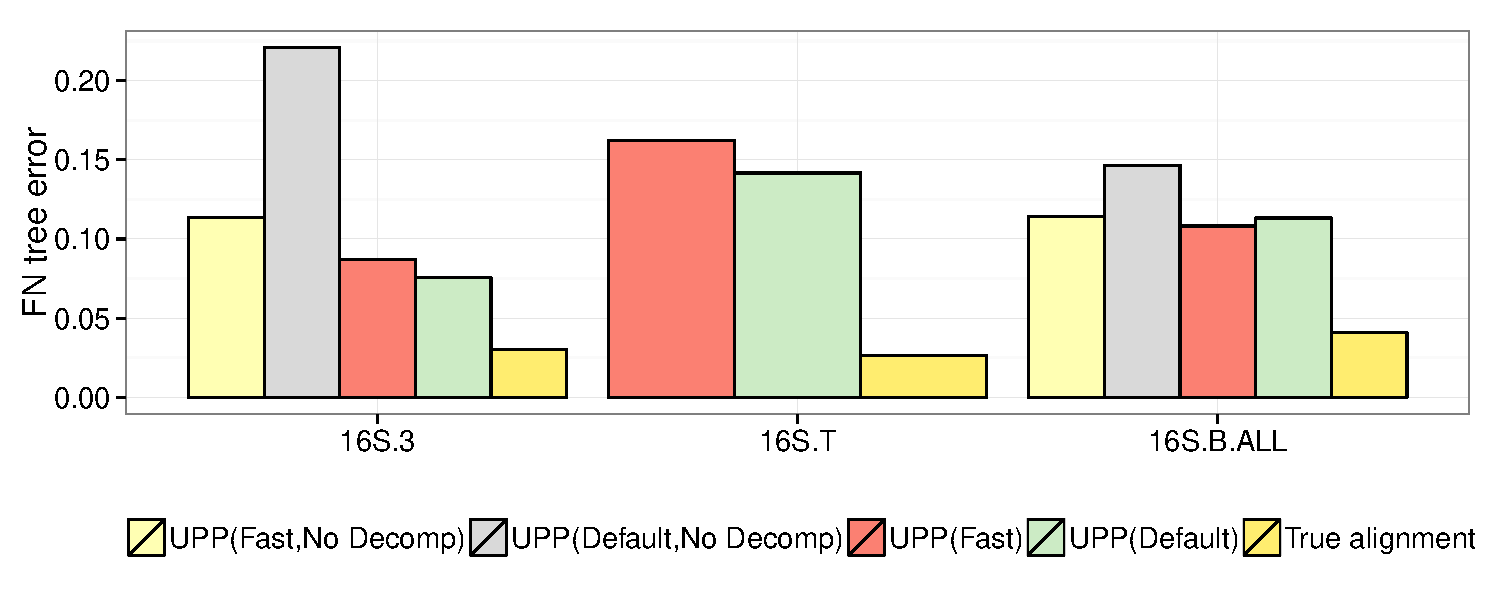
\includegraphics[width=0.90\linewidth]{{upp/gutell.upp.fn}.pdf}\\
  \caption[]{FN tree error}
\end{subfigure}
\begin{subfigure}[htpb]{\textwidth}
  \centering
  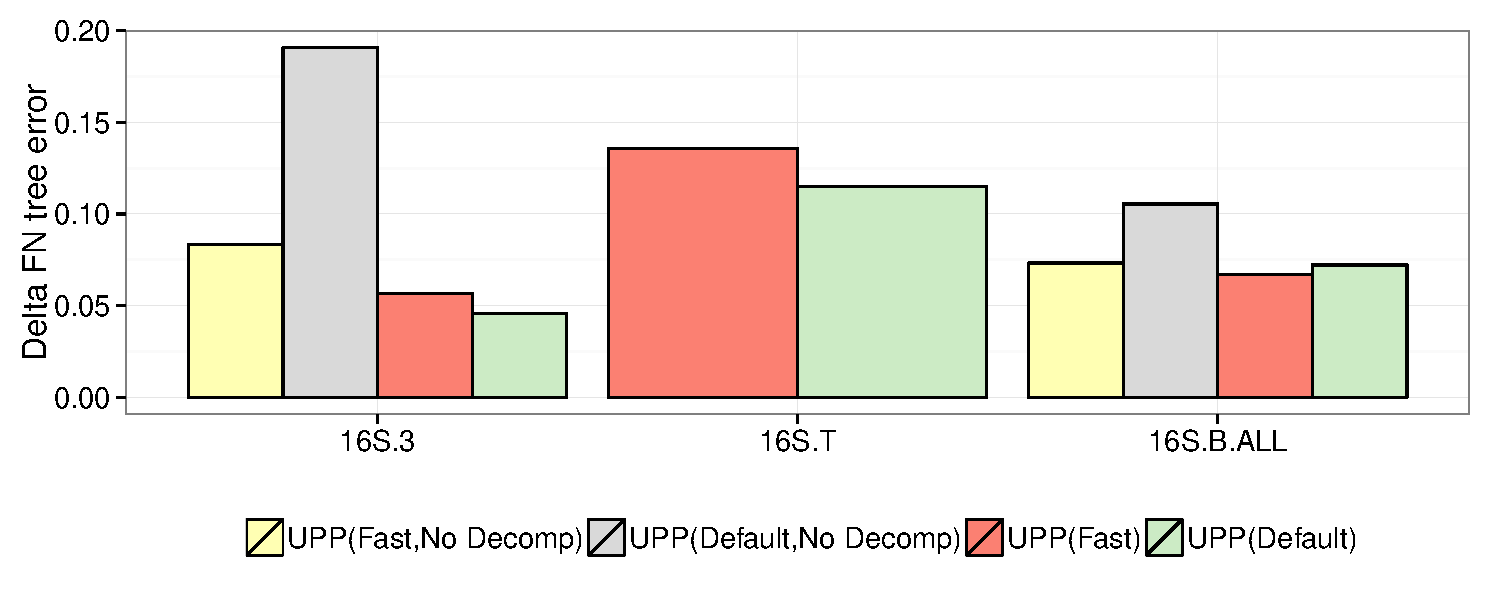
\includegraphics[width=0.90\linewidth]{{upp/gutell.upp.delta_fn}.pdf}\\
  \caption[]{Delta FN tree error}
\end{subfigure}
\caption[Tree error of UPP variants on the CRW 16S datasets.]{\label{gutell_upp_tree}  {\bf Tree error of UPP variants on the CRW 16S datasets.}  ML trees were estimated using FastTree under GTR.  Methods labeled with ``Default'' use a backbone size of 1000.  Methods labeled with ``Fast'' use a backbone size of 100.  Both UPP(Default,No Decomp) and UPP(Fast,No Decomp) failed to align one of the 16S.T sequences and thus failed to generate an alignment on the entire dataset.  UPP results are based on the first iteration of UPP.}
\end{figure}
%Nam - is this two iterations or one?
%One iteration, we didn't have time to iterate on all the 16S.T variants, i.e., we would also need to iterate on UPP(Fast) if we plan to apply it everywhere

\begin{figure}[htpb]
\centering
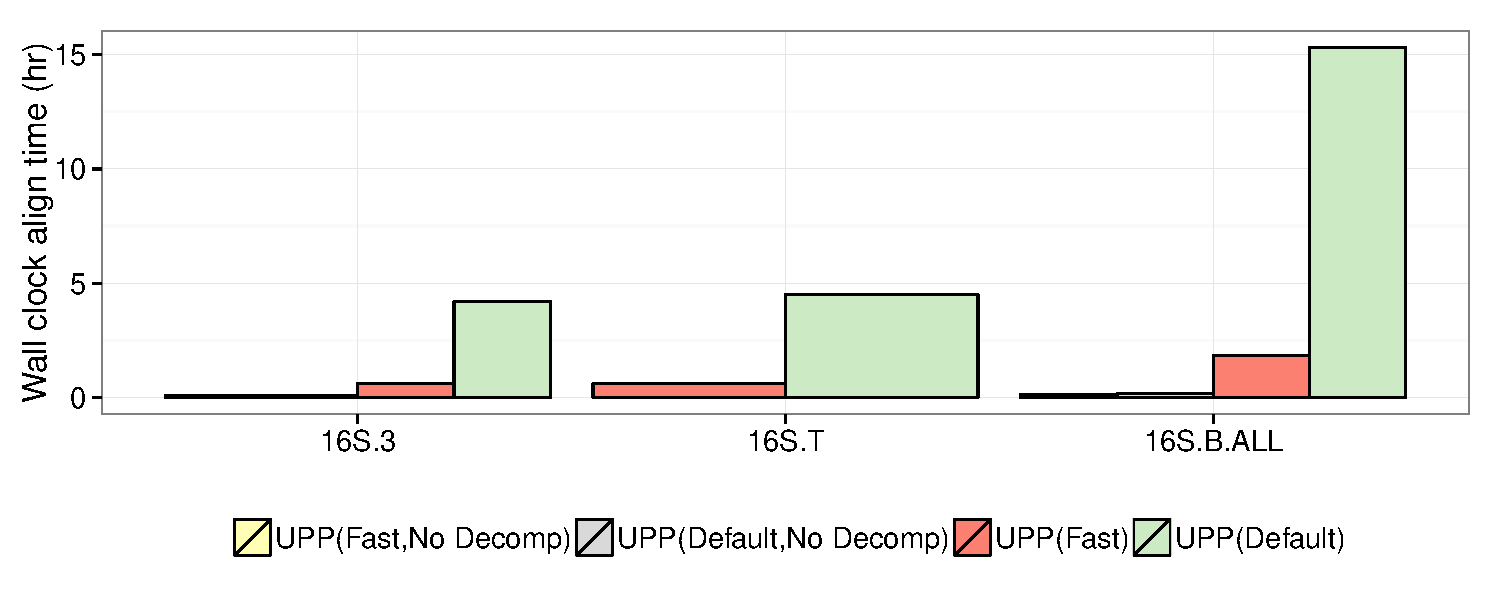
\includegraphics[width=0.90\linewidth]{{upp/gutell.upp.wall_align_time}.pdf}\\
\caption[Wall clock alignment time (hrs) of UPP variants on the
RNASim datasets.]{\label{gutell_upp_time}  {\bf  Wall clock alignment time (hrs) of UPP variants on the RNASim datasets.}  
All methods were run on a machine with 12 CPUs and 24 GB of memory.  UPP(Default) uses a backbone of size 1000.  UPP(Fast) uses a backbone of size 100. Both UPP(Default,No Decomp) and UPP(Fast,No Decomp) failed to align one of the 16S.T sequences and thus failed to generate an alignment on the entire dataset.  UPP results are based on the first iteration of UPP.}
\end{figure}
\clearpage
\subsection{SEPP vs.~UPP}\label{upp_sepp}
We now compare UPP and SEPP. Recall that both methods use
the same backbone, but SEPP divides the dataset into approximately
ten disjoint subsets of approximately equal size, and constructs
HMMs on each subset alignment.  In comparison,
UPP uses the HMM Family technique, which will produce a much larger
collection of HMMs.

SEPP(Default,10\%) and UPP(Default) use the same
backbone alignment, but SEPP decomposes the alignment
into disjoint subsets (approximately 10 of them), using the
centroid edge decomposition from SAT\'e-II;
``10\%" refers to the requirement that every subset should have
approximately 10\% of the backbone sequences, the protocol
used in \cite{Mirarab2012}.

Both UPP and SEPP had comparable alignment accuracy on both the RNASim and CRW 16S datasets (Figs.~\ref{rnasim_sepp_alignment}-\ref{gutell_sepp_alignment}).  Differences between the methods were more distinct on the CRW 16S datasets, especially with respect to tree accuracy.  UPP resulted in significantly better trees on all of the CRW datasets (Fig.~\ref{gutell_sepp_tree}).  In addition, UPP was more robust to fragmentary datasets compared to SEPP (Fig. \ref{fig:frag_sepp}).


\begin{figure}[htpb]
\begin{subfigure}[htpb]{\textwidth}
  \centering
  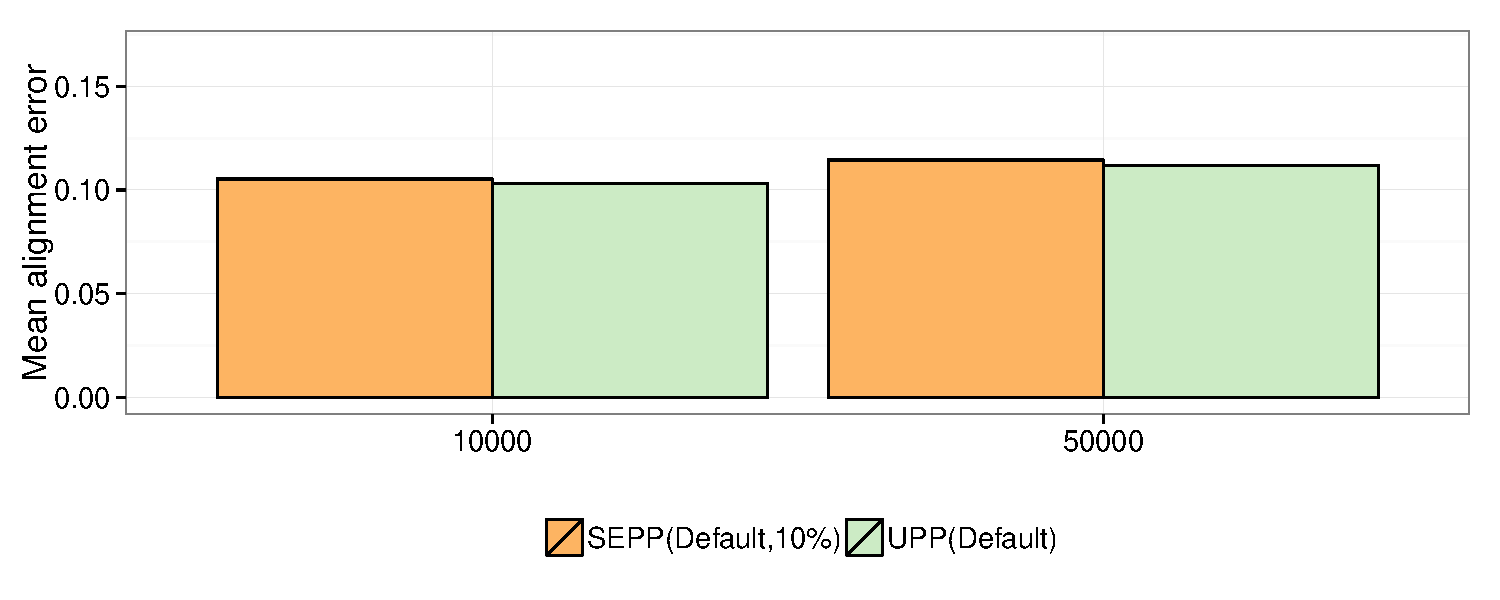
\includegraphics[width=0.70\linewidth]{{upp/rnasim.sepp.alignment_average}.pdf}\\
  \caption[]{Average alignment error}
\end{subfigure}
\begin{subfigure}[htpb]{\textwidth}
  \centering
  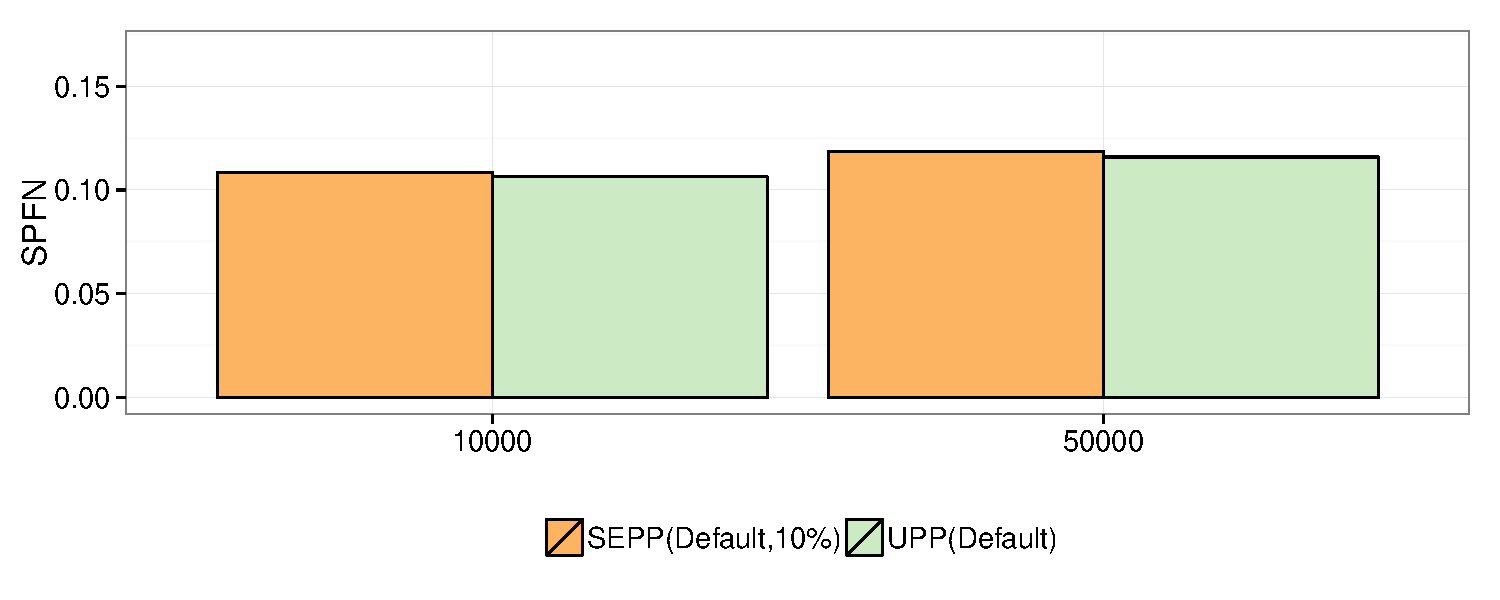
\includegraphics[width=0.70\linewidth]{{upp/rnasim.sepp.spfn}.pdf}\\
  \caption[]{Alignment SPFN error}
\end{subfigure}
\begin{subfigure}[htpb]{\textwidth}
  \centering
  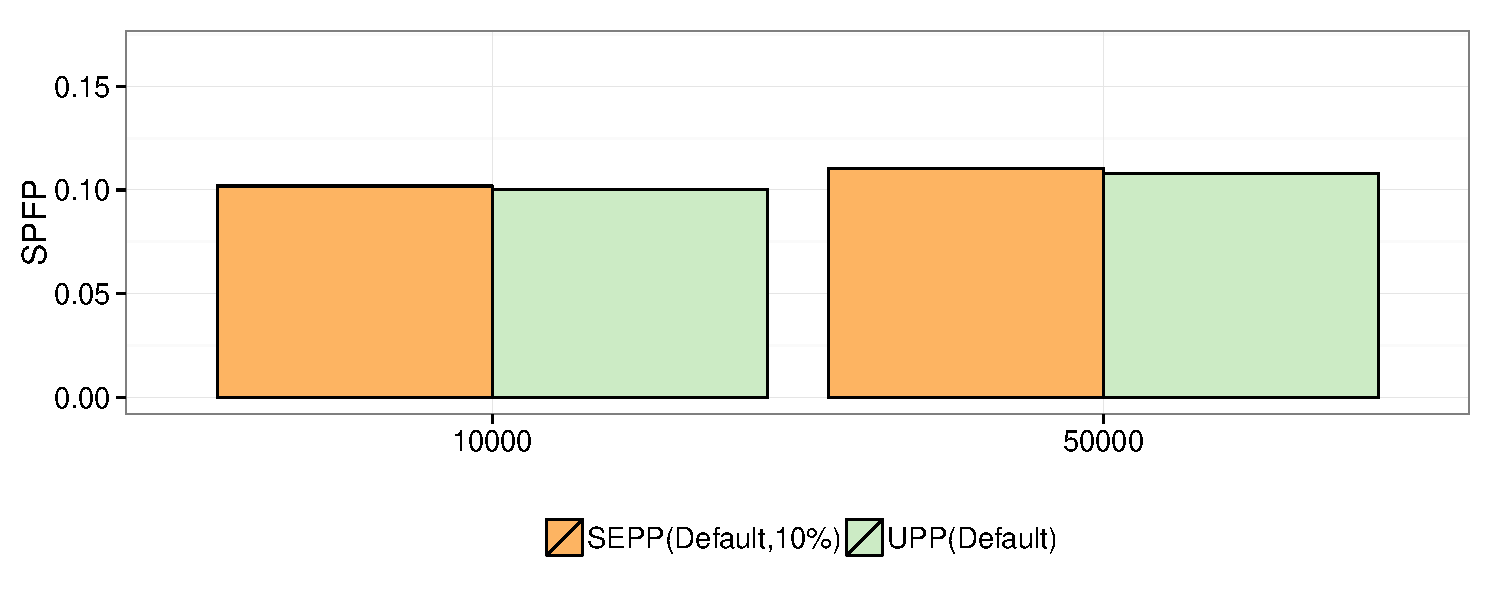
\includegraphics[width=0.70\linewidth]{{upp/rnasim.sepp.spfp}.pdf}\\
  \caption[]{Alignment SPFP error}
\end{subfigure}
\caption[Alignment error of UPP and SEPP on the
RNASim datasets.]{\label{rnasim_sepp_alignment}  {\bf Alignment
error for UPP and SEPP on the RNASim datasets with 10K and 50K sequences.}  
UPP(Default) and SEPP(Default,10\%) both use the same  backbone of size 1000. 
SEPP decomposes the backbone into (approximately) 10 subsets each of the same size.
}
\end{figure}

\begin{figure}[htpb]
\begin{subfigure}[htpb]{\textwidth}
  \centering
  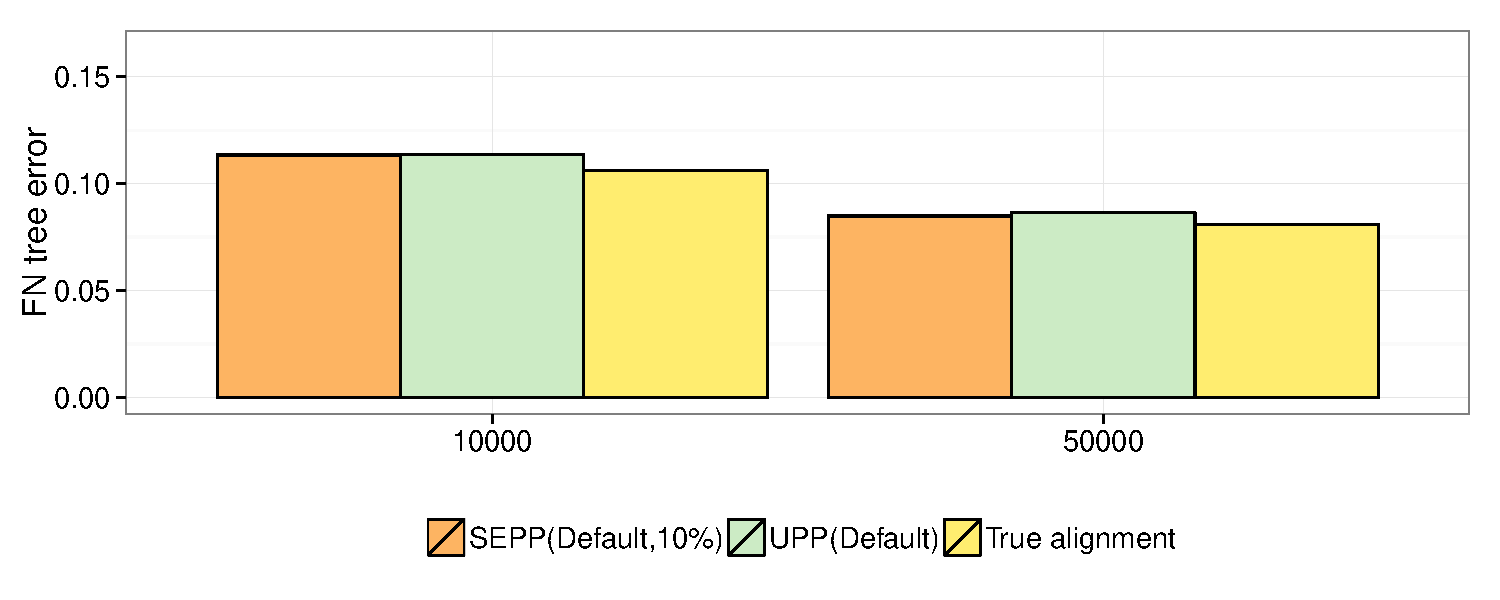
\includegraphics[width=0.90\linewidth]{{upp/rnasim.sepp.fn}.pdf}\\
  \caption[]{FN tree error}
\end{subfigure}
\begin{subfigure}[htpb]{\textwidth}
  \centering
  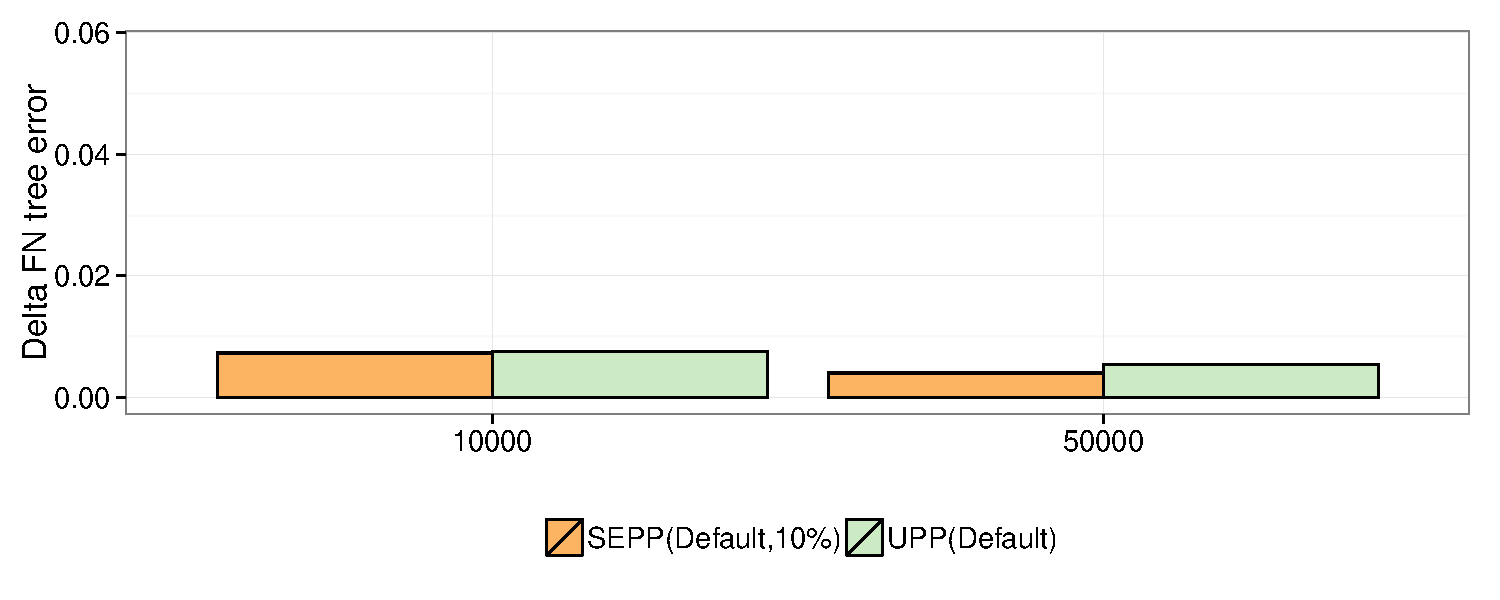
\includegraphics[width=0.90\linewidth]{{upp/rnasim.sepp.delta_fn}.pdf}\\
  \caption[]{Delta FN tree error}
\end{subfigure}
\caption[Tree error of UPP and SEPP on the RNASim datasets.]{\label{rnasim_sepp_tree}  
{\bf Tree error of UPP and SEPP on the RNASim datasets with
10K and 50K sequences.}  ML trees were estimated using FastTree under GTR.  
UPP(Default) and SEPP(Default,10\%)  both use the same backbone of size 1000.  
SEPP(Default,10\%) decomposes the backbone into (approximately) 10 subsets each of the same size.}
\end{figure}

\begin{figure}[htpb]
\begin{subfigure}[htpb]{\textwidth}
  \centering
  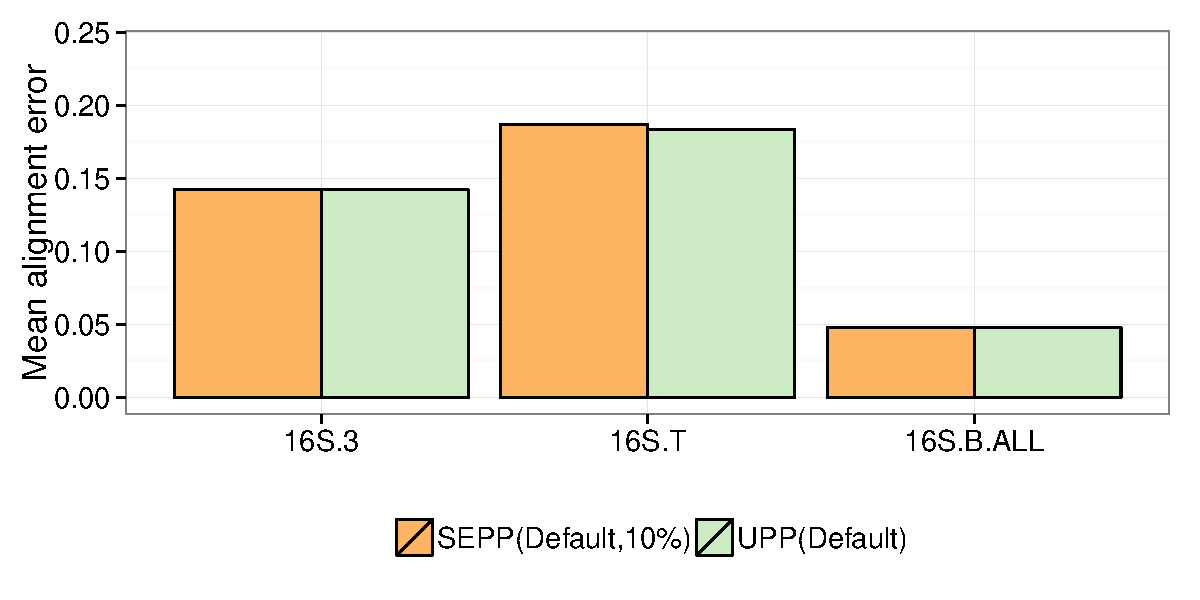
\includegraphics[width=0.70\linewidth]{{upp/gutell.sepp.alignment_average}.pdf}\\
  \caption[]{Average alignment error}
\end{subfigure}
\begin{subfigure}[htpb]{\textwidth}
  \centering
  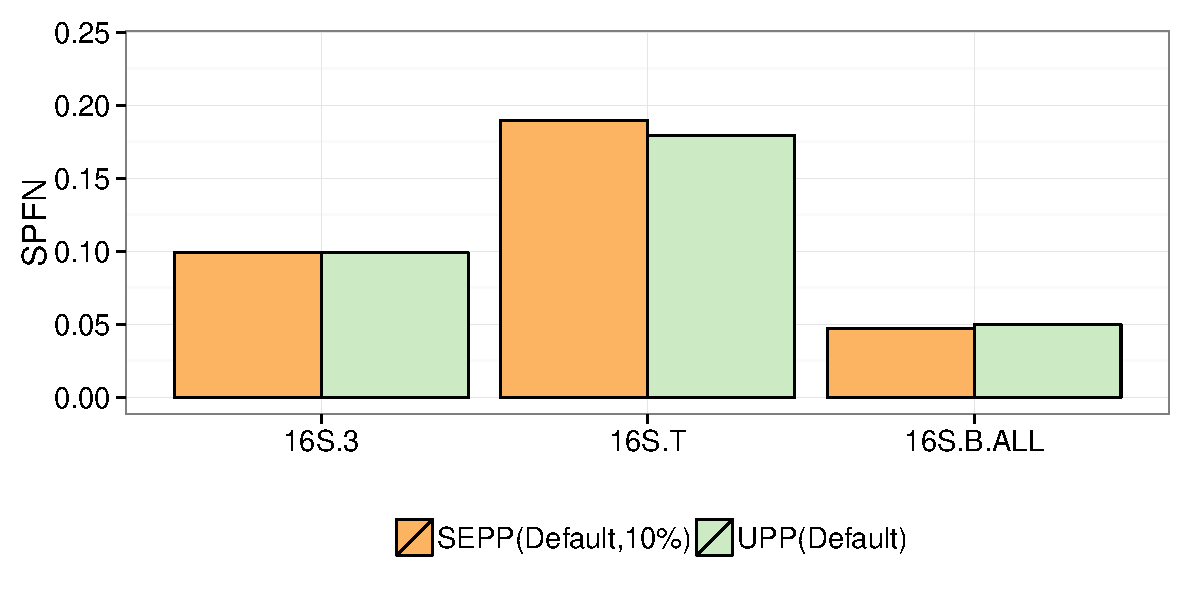
\includegraphics[width=0.70\linewidth]{{upp/gutell.sepp.spfn}.pdf}\\
  \caption[]{Alignment SPFN error}
\end{subfigure}
\begin{subfigure}[htpb]{\textwidth}
  \centering
  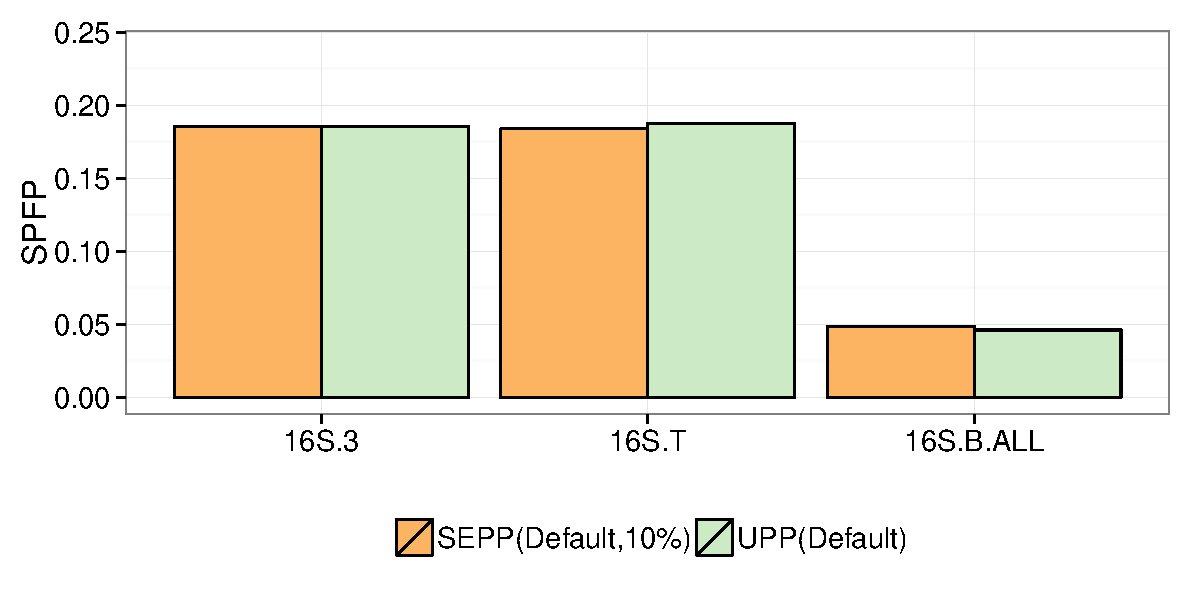
\includegraphics[width=0.70\linewidth]{{upp/gutell.sepp.spfp}.pdf}\\
  \caption[]{Alignment SPFP error}
\end{subfigure}
\caption[Alignment error of UPP and SEPP on the
CRW 16S datasets.]{\label{gutell_sepp_alignment}  {\bf Alignment
error for UPP and SEPP on the CRW 16S datasets.}  
UPP(Default) and SEPP(Default,10\%)  both use the same backbone of size 1000.
SEPP(Default,10\%) decomposes the backbone into (approximately) 10 subsets each of the same size.  UPP and SEPP results shown are based on the first iteration.
%Nam - update with two iterations of UPP
%Wouldn't be fair comparison because we would need two iterations of UPP for everything.
}

\end{figure}

\begin{figure}[htpb]
\begin{subfigure}[htpb]{\textwidth}
  \centering
  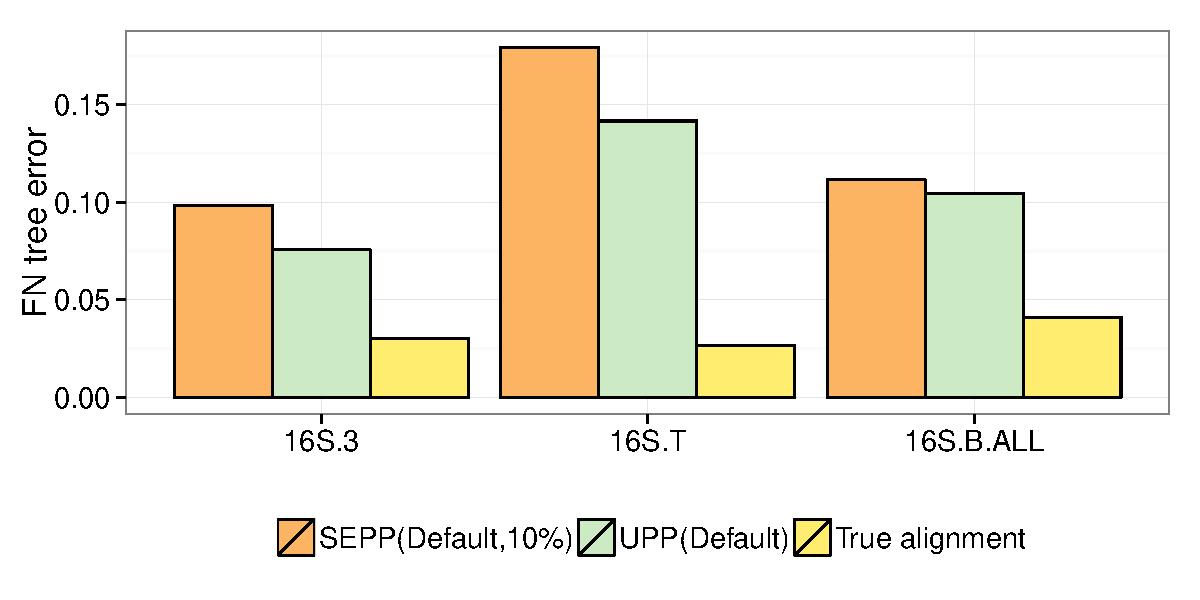
\includegraphics[width=0.90\linewidth]{{upp/gutell.sepp.fn}.pdf}\\
  \caption[]{FN tree error}
\end{subfigure}
\begin{subfigure}[htpb]{\textwidth}
  \centering
  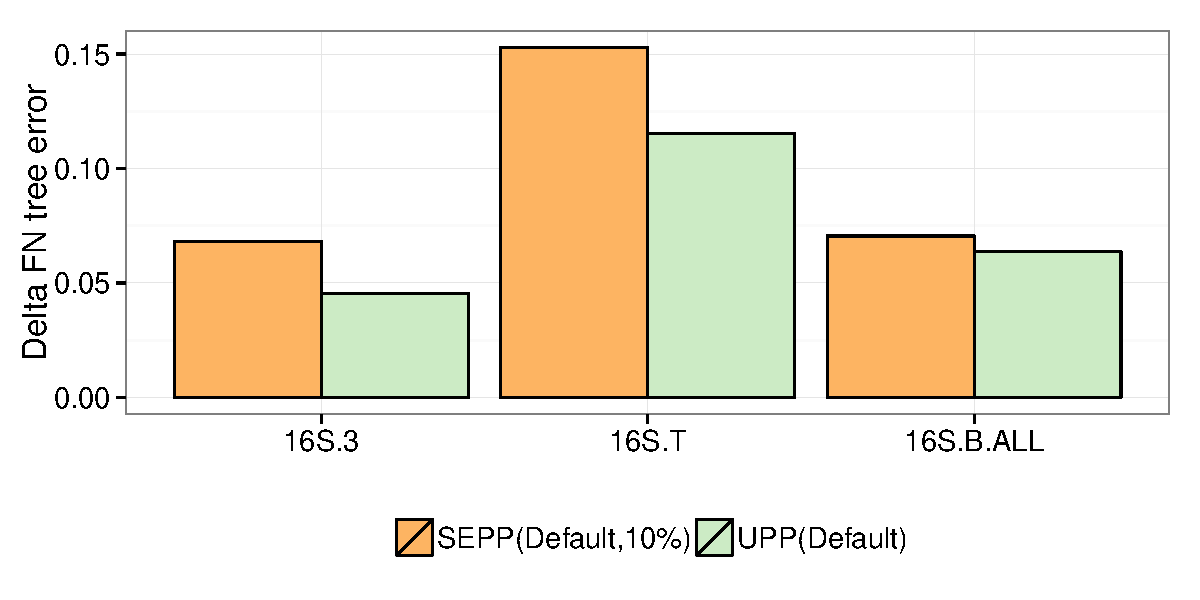
\includegraphics[width=0.90\linewidth]{{upp/gutell.sepp.delta_fn}.pdf}\\
  \caption[]{Delta FN tree error}
\end{subfigure}
\caption[Tree error of UPP and SEPP on the CRW 16S datasets.]{\label{gutell_sepp_tree}  {\bf Tree error of UPP and SEPP on the CRW 16S datasets.}  ML trees were estimated using FastTree under GTR. 
UPP(Default) and SEPP(Default,10\%)  both use the same backbone of size 1000.
SEPP(Default,10\%) decomposes the backbone into (approximately) 10 subsets each of the same size.  UPP and SEPP results shown on 16S.T are based off of one iteration.
}
\end{figure}


\begin{figure}[htpb]
\begin{subfigure}[htpb]{\textwidth}
  \centering
  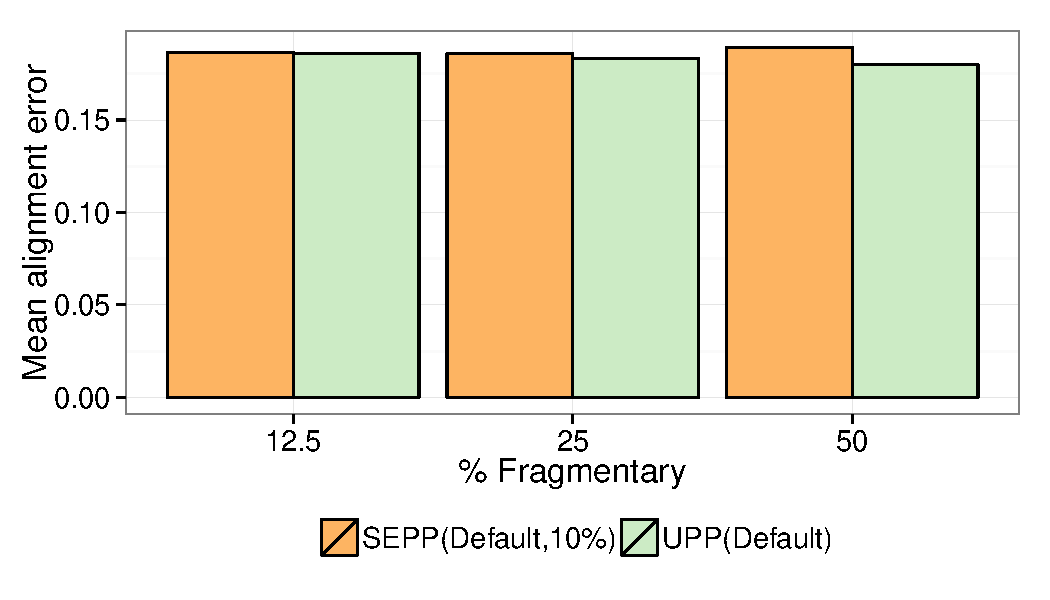
\includegraphics[width=0.85\linewidth]{{upp/frag.16S.T.alignment_average.sepp.500}.pdf}\\  
  \caption[]{Average alignment error}
\end{subfigure}
\begin{subfigure}[htpb]{\textwidth}
  \centering
  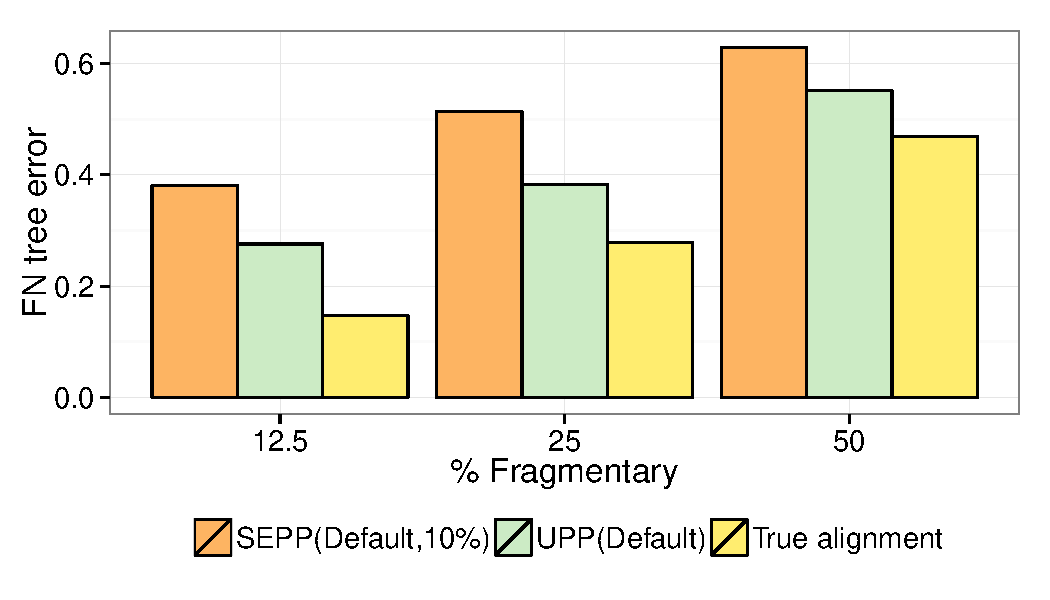
\includegraphics[width=0.85\linewidth]{{upp/frag.16S.T.fn.sepp.500}.pdf}\\  
  \caption[]{Tree error}
\end{subfigure}
\caption[Alignment and tree error for SEPP and UPP on fragmentary CRW 16S.T datasets.]{\label{fig:frag_sepp}  
{\bf Alignment and tree error for SEPP and UPP on fragmentary CRW 16S.T datasets.}
We show alignment error and tree error for UPP and SEPP on the 
fragmentary CRW 16S.T datasets, varying 
the percentage of fragmentary sequences, each with an average 
length of 500 sites 
(i.e., approximately one third the average sequence length for 16S.T).
UPP(Default) and SEPP(Default,10\%)  both use the same backbone of size 1000.
SEPP(Default,10\%) decomposes the backbone into (approximately) 10 subsets each of the same size.  UPP results are based on the first iteration of UPP.
} 
\end{figure}
\clearpage

\subsection{MAFFT variants\label{mafft_variant}}
We compared MAFFT-PartTree and MAFFT-Default on the large datasets.  Fig.~\ref{mafft_default_parttree} shows that MAFFT-PartTree results in comparable or better alignments than default MAFFT, however, default MAFFT results in significantly better trees.  

\begin{figure}[htpb]
\begin{subfigure}[htpb]{\textwidth}
  \centering
  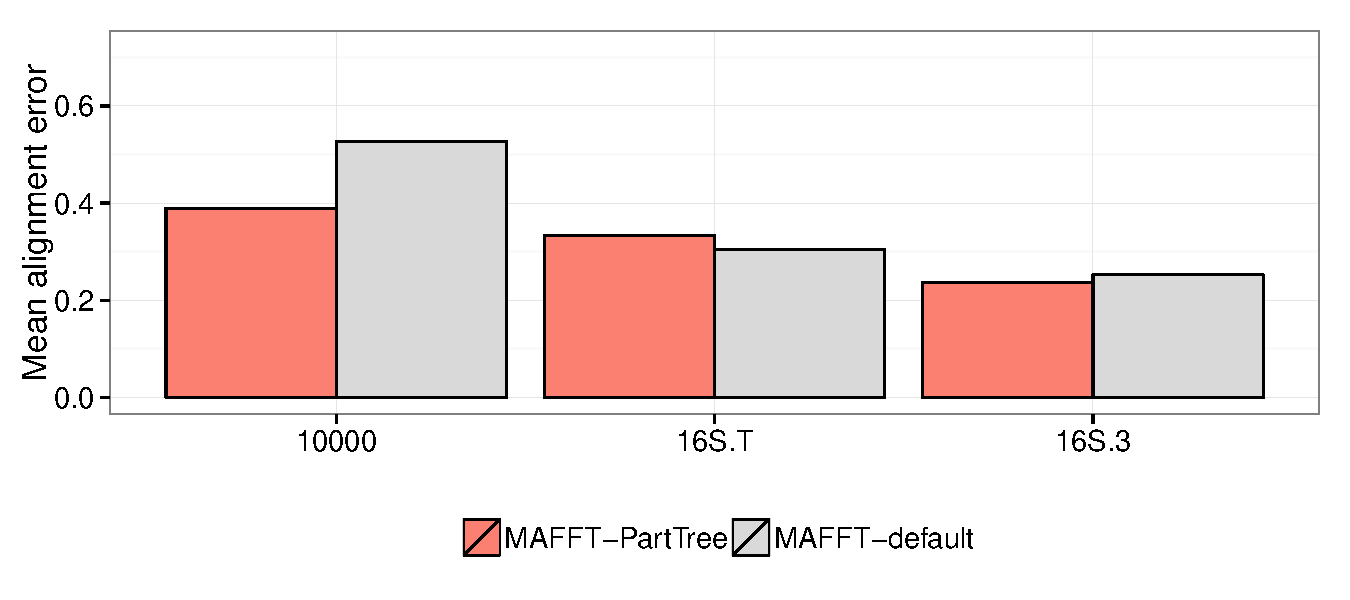
\includegraphics[width=0.9\linewidth]{{upp/rnasim.mafft_variant.alignment_average}.pdf}\\
  \caption[]{Average alignment error}
\end{subfigure}
\begin{subfigure}[htpb]{\textwidth}
  \centering
  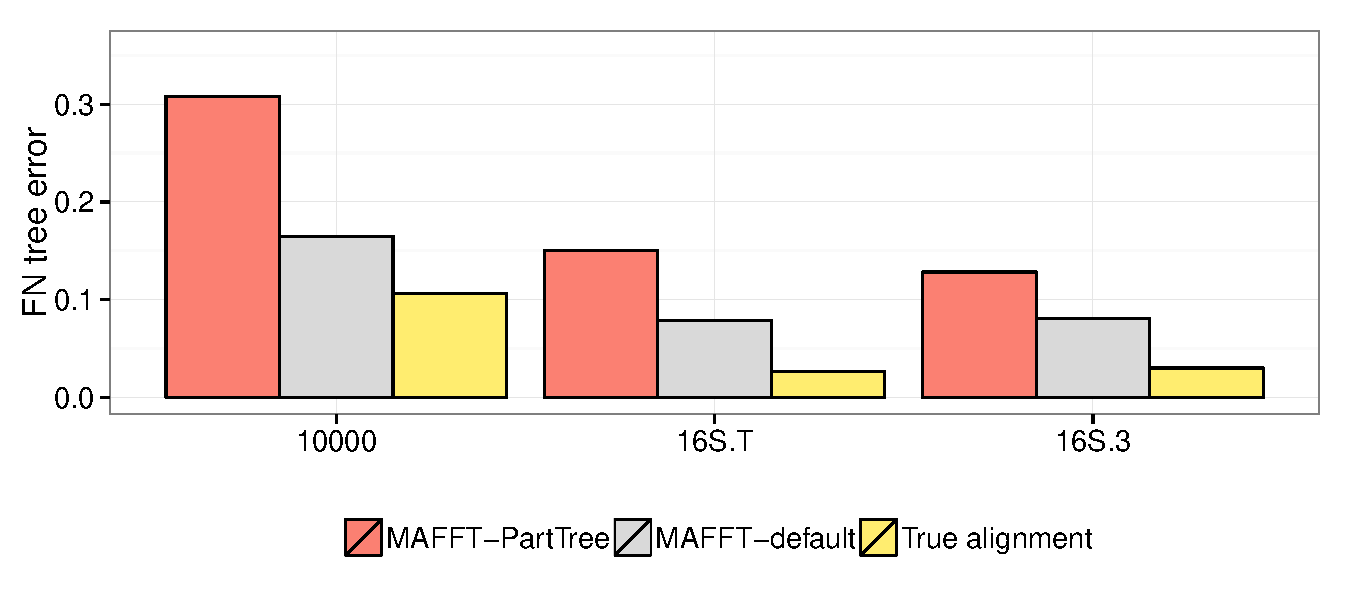
\includegraphics[width=0.9\linewidth]{{upp/rnasim.mafft_variant.fn}.pdf}\\
  \caption[]{FN tree error}
\end{subfigure}
\caption[Results of default MAFFT and MAFFT-PartTree on the
16S.T, 16S.3, and RNASim 10K
datasets.]{\label{mafft_default_parttree}  
{\bf Results of default MAFFT and MAFFT-PartTree on the
16S.T, 16S.3, and RNASim 10K
datasets.}  All ML trees were estimated using FastTree under GTR.}  
\end{figure}

\clearpage
%{\bf Nam - take out MAFFT-Profile}

% \begin{figure}[htpb]
% \begin{subfigure}[htpb]{\textwidth}
  % \centering
  % 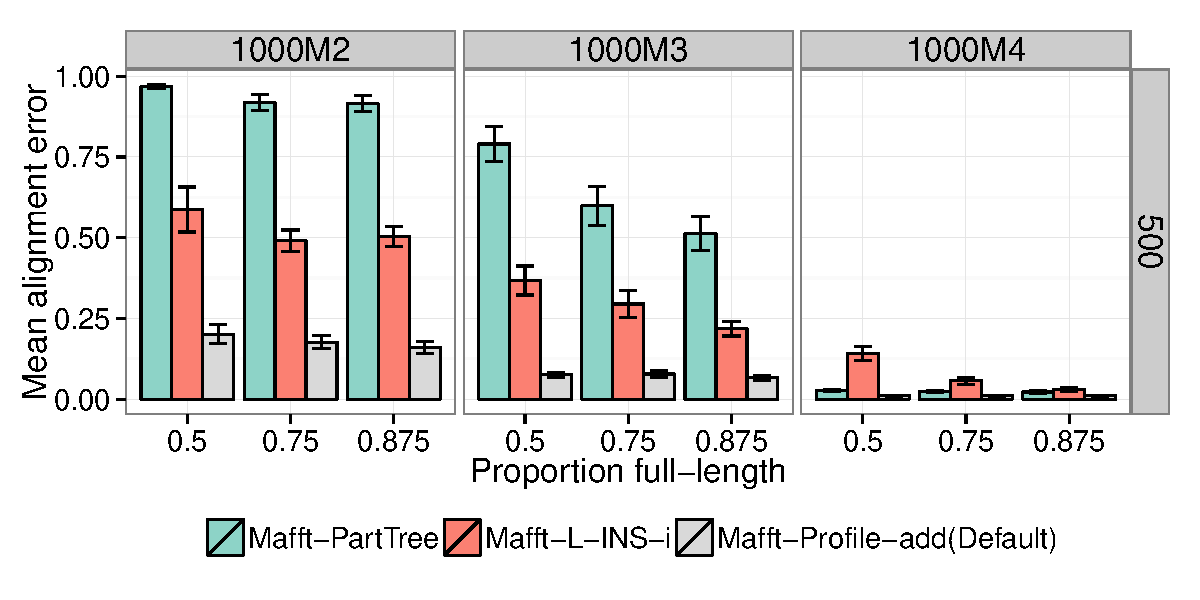
\includegraphics[width=0.9\linewidth]{{upp/1000_taxa_fragments_alignment_mean.mafft}.pdf}\\
  % \caption[]{Average alignment error}
% \end{subfigure}
% \begin{subfigure}[htpb]{\textwidth}
  % \centering
  % 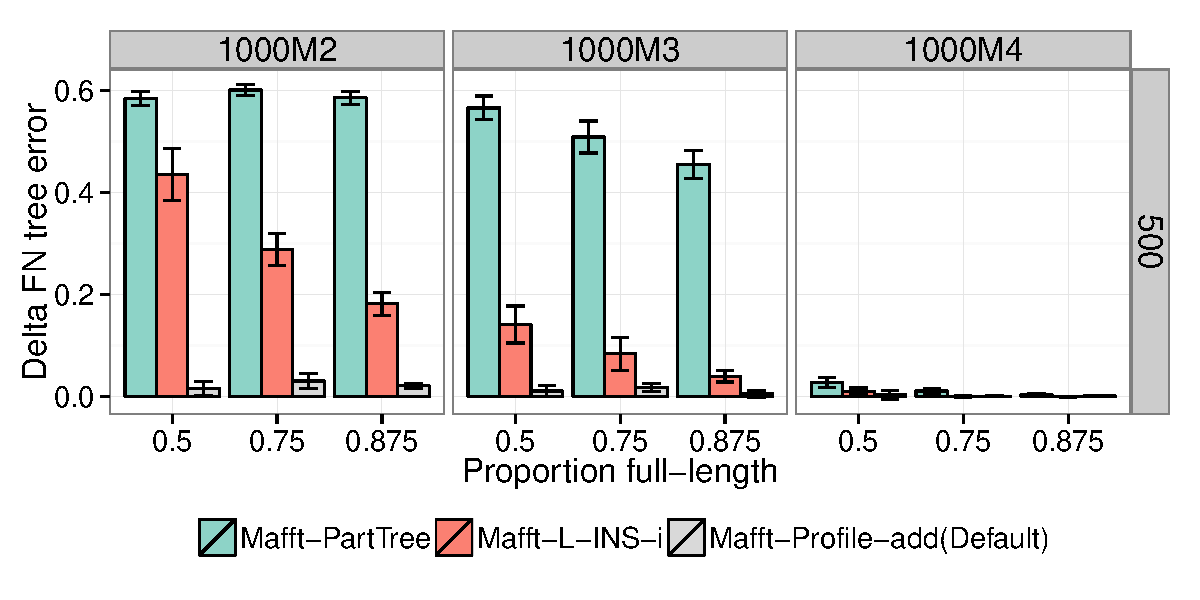
\includegraphics[width=0.9\linewidth]{{upp/1000_taxa_fragments_delta_fn.mafft}.pdf}\\
  % \caption[]{Delta tree error}
% \end{subfigure}
% \caption[Results of MAFFT variants on the fragmentary
% 1000-taxon datasets.]{\label{small_frag_mafft}  
% {\bf  Results of MAFFT variants on the fragmentary 1000-taxon datasets.}  
% All ML trees were estimated using FastTree.  Fragmentary sequences were simulated with an average fragment length of 500 bps (i.e., half length).  Backbone sequences were selected from all sequences that were within 1000 bps $\pm$ 250 bps in length.  Standard error bars are shown.  Averages are computed over 5 replicates per dataset.}
% \end{figure}

\clearpage

\subsection{PASTA on the ten large AA datasets}\label{pasta_protein}
UPP's alignment accuracy depends on the accuracy of the backbone alignment.  
PASTA is an improvement on SAT\'e-II, and both have
been  studied extensively on NT datasets \cite{PASTA}; however, 
no published studies have studied PASTA, SAT\'e-I or SAT\'e-II on AA datasets.  


We explored PASTA variants, varying the technique used to estimate alignments on
subsets and then to merge alignments together, using the 10 AA datasets with full
reference alignments.
Initial analyses (data not shown) revealed that MAFFT-L-INS-i gave the best results
for producing the subset alignments.
We then evaluated techniques for merging alignments, including
Opal~\cite{Wheeler2007}, MUSCLE~\cite{Edgar2004}, or COBALT~\cite{Papadopoulos2007}.
% was used to merge the subalignments; all other parameters were fixed.  

We ran PASTA under default settings (no starting tree, subset size 200, MAFFT-L-INS-i
to align subsets, FastTree to compute trees in each
iteration, and running for three iterations), varying only the
alignment merger technique.
The software version numbers and commands used within PASTA to align the sequences and merge the subsets are given in Section~\ref{pasta_commands}.  ML trees were estimated on the alignments using RAxML under JTT, LG, or WAG models of protein evolution (model selection described in Section~\ref{model_selection_pasta}).

We found that while all PASTA variants resulted in alignments with  comparable accuracy, 
RAxML maximum likelihood trees on PASTA using MUSCLE to merge subalignments 
resulted in the most accurate trees (Fig. ~\ref{kk_pasta}).  
We refer to this version as ``PASTA-MUSCLE."

We then compared PASTA-MUSCLE to alignments and trees computed using
standard MSA methods followed by RAxML for maximum likelihood.
PASTA-MUSCLE and MAFFT-L-INS-i gave the most accurate alignments, 
but PASTA-MUSCLE resulted in the most accurate trees (Fig. ~\ref{kk_twophase}).  Thus, we used PASTA-MUSCLE to generate our backbone alignments for AA datasets.


\begin{figure}[htpb]
\begin{subfigure}[htpb]{\textwidth}
  \centering
  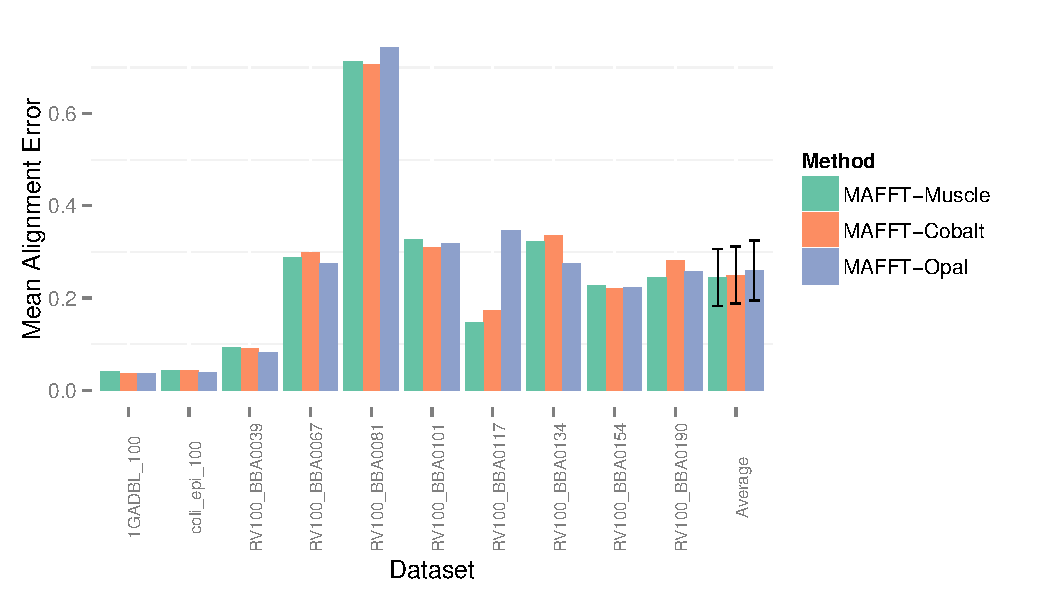
\includegraphics[width=.90\linewidth]{{upp/PASTA_SP}.pdf}\\
  \caption[]{Mean alignment error of PASTA variants}
\end{subfigure}
\begin{subfigure}[htpb]{\textwidth}
  \centering
  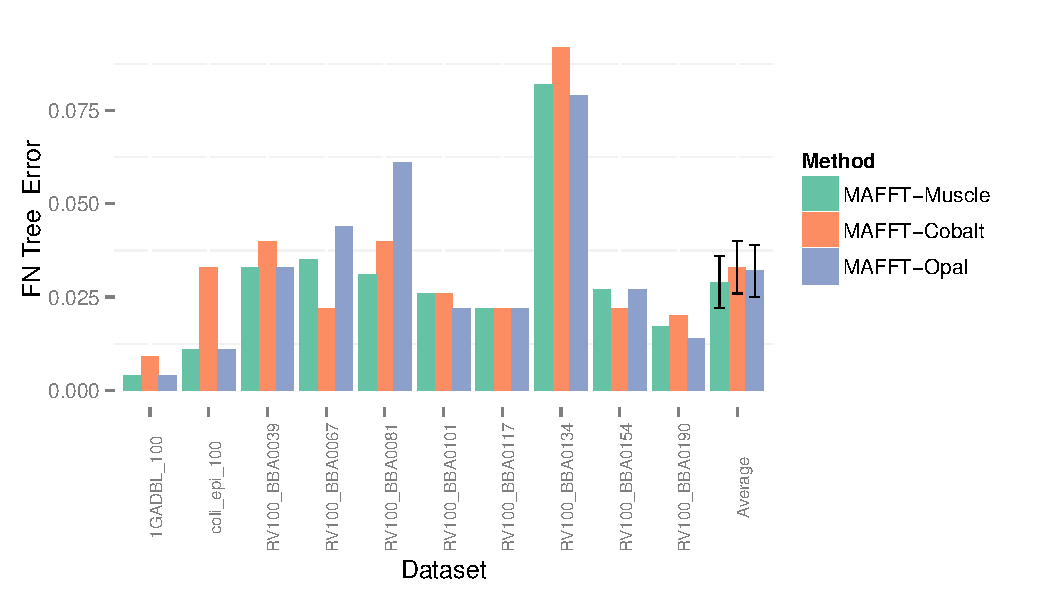
\includegraphics[width=.90\linewidth]{{upp/PASTA_FN}.pdf}\\
  \caption[]{Tree FN error of PASTA variants}
\end{subfigure}
\caption[Alignment and tree error of PASTA variants on the ten large AA datasets with
full reference alignments, using substitution models selected by PROTEST.]{\label{kk_pasta}  
{\bf Alignment and tree error for PASTA variants on the ten large AA datasets with
full reference alignments.}  Subalignments were estimated using MAFFT-L-INS-i, and the resulting subalignments were merged with either MUSCLE, Opal, or Cobalt.  ML Trees were estimated using RAxML under amino acid substitution models selected using PROTEST (see Section~\ref{model_selection_pasta}).}
\end{figure}

\begin{figure}[htpb]
\begin{subfigure}[htpb]{\textwidth}
  \centering
  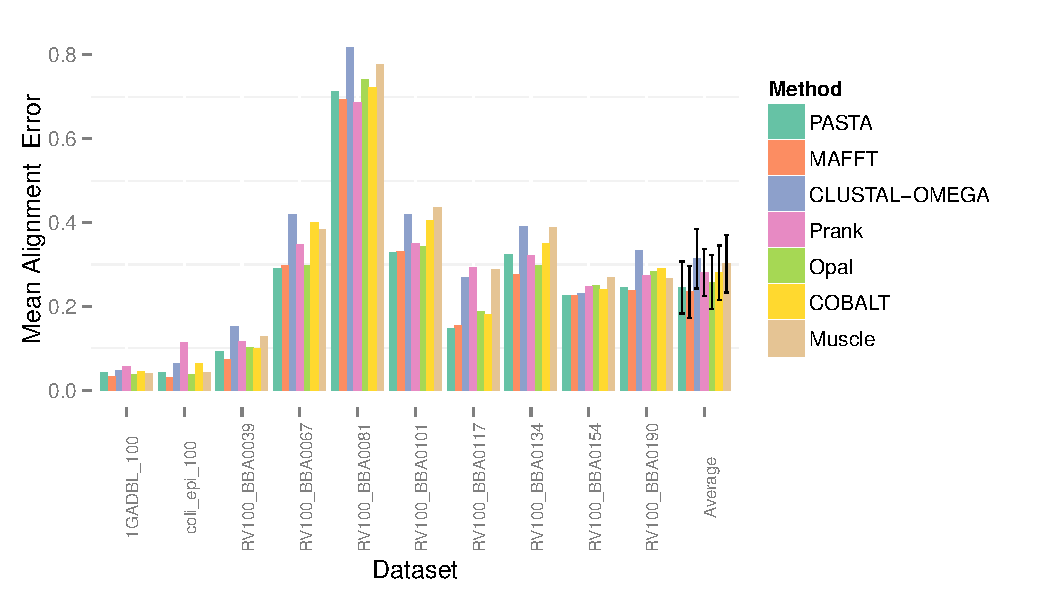
\includegraphics[width=.90\linewidth]{{upp/Balibase_SP}.pdf}\\
  \caption[]{Mean alignment error }
\end{subfigure}
\begin{subfigure}[htpb]{\textwidth}
  \centering
  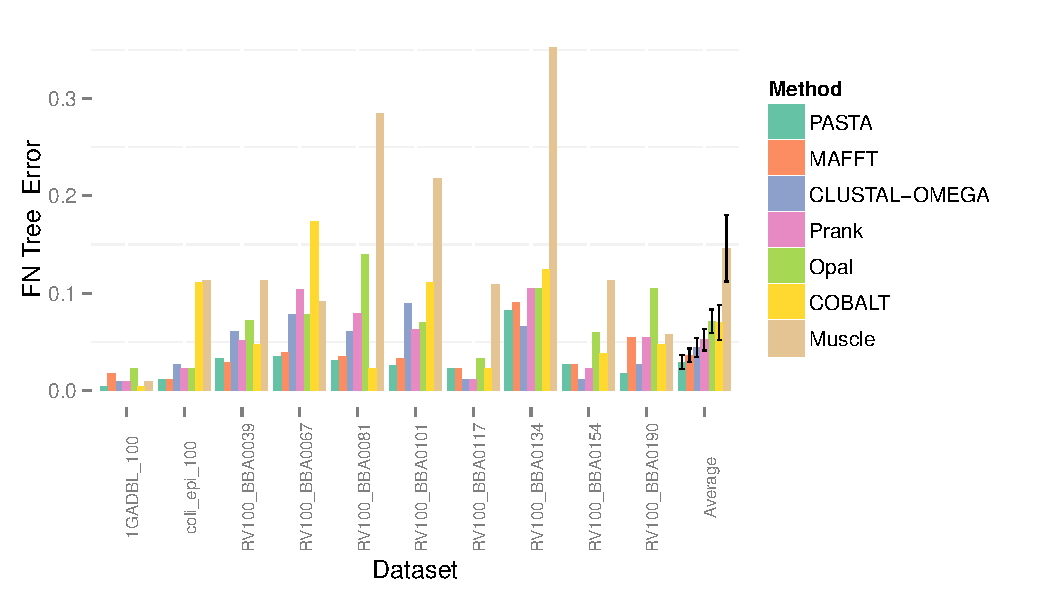
\includegraphics[width=.90\linewidth]{{upp/Balibase_FN}.pdf}\\
  \caption[]{Tree FN error }
\end{subfigure}
\caption[Alignment and tree error of different methods on the ten large AA datasets with
full reference alignments,
using substitution models selected by PROTEST.]{\label{kk_twophase}  {\bf Alignment and tree error of different methods on the ten large AA datasets with full reference alignments.}  PASTA used MAFFT-L-INS-i to align subalignments, and MUSCLE to merge subalignments.  ML Trees were estimated using RAxML under amino acid substitution models selected using PROTEST (see Section~\ref{model_selection_pasta}).}
\end{figure}
\clearpage

\subsubsection{PASTA commands}\label{pasta_commands}
The following software was used to generate the results presented in Section ~\ref{pasta_protein}:

Each dataset was aligned (when possible) using Opal \cite{Wheeler2007} version 2.0.0, Clustal-Omega \cite{Sievers2011} version 1.0.2, MAFFT\cite{Katoh2002,Katoh2005,Katoh2012} version 6.857b, Cobalt \cite{Papadopoulos2007} version 2.0.1, MUSCLE \cite{Edgar2004,Edgar2004a} version 3.8.31, PRANK \cite{Loytynoja2005} version 100802 and PASTA version 1.0 \cite{PASTA}.  Due to a bug in earlier versions of MAFFT 6.956b, MAFFT-Profile and MAFFT-default were run using MAFFT version 7.143.


The commands used for the experiments in Section~\ref{pasta_protein} are given below.
\begin{itemize}
\item \textbf{Clustal-Omega}:~\emph{clustalo -align -i$<$input\_sequence$>$ -o $<$output\_alignment$>$}
\item \textbf{MAFFT}:~\emph{mafft -{}-localpair -{}-maxiterate 1000 -{}-ep 0.123 $<$input\_sequence$>$ $>$ $<$output\_alignment$>$}
\item \textbf{Opal}:~\emph{java -Xmx20g -jar opal.jar -{}-in $<$input\_sequences$>$ -{}-out $<$output\_alignment$>$}
\item \textbf{MUSCLE}:~\emph{muscle -in $<$input\_sequence$>$ -out $<$output\_alignment$>$}
\item \textbf{Cobalt}:~\emph{cobalt -i $<$input\_sequence$>$ -rpsdb $<$cdd\_clique\_0.75$>$ $>$ output\_alignment$>$}
\item \textbf{Prank}:~\emph{prank -once -noxml -notree -nopost +F -quiet -matinitsize=5 -protein -d=$<$input\_sequence$>$ -o=$<$output\_alignement$>$}
\item \textbf{RaxML}:~\emph{raxml -m PROTGAMMA$<$model$>$ -n ml -s $<$output\_phylip$>$ -T2 -w $<$working\_directory$>$}
\item \textbf{PASTA}:~\emph{python run\_pasta.py -o $<$output\_directory$>$ -i  $<$input\_sequences$>$ -t $<$starting\_tree$>$ -{}-auto -{}-num-cpus=12 -{}-datatype=$<$molecule\_type$>$}
\end{itemize}
\clearpage
\subsubsection{Model selection for PASTA variants}\label{model_selection_pasta}
Model selection for the ten large AA datasets with full reference
alignments was performed with PROTEST, using the input parameters listed below:
\begin{verbatim}
  Alignment file........... : [MAFFT-L-INS-i alignment]
  Tree..................... :RAxML parsimony tree on 
                             MAFFT-L-INS-i
  StrategyMode............. : Fast (optimize branch lengths & model)
  Candidate models......... : 
    Matrices............... : JTT LG WAG 
    Distributions.......... : +G 
    Number of rate categ... : 4
    Observed frequencies... : false
  Statistical framework
    Sort models according to....: AIC
    Sample size.................: 0.0 (not calculated yet)
      sampleSizeMode............: Total number of characters 
                                  (aligment length)
\end{verbatim}

PROTEST selected the following AA models for the 10 AA datasets:
\begin{itemize}
\item 1GADBL\_100: LG
\item coli\_epi\_100: LG
\item RV100\_BBA0039: LG
\item RV100\_BBA0067: WAG
\item RV100\_BBA0081: JTT
\item RV100\_BBA0101: WAG
\item RV100\_BBA0117: LG
\item RV100\_BBA0134: JTT
\item RV100\_BBA0154: WAG
\item RV100\_BBA0190: LG
\end{itemize}

\clearpage
\subsection{Comparisons between UPP, SAT\'e-II, and PASTA}\label{sec:som-upp-vs-pasta}
We compared UPP to SAT\'e-II and PASTA on both full-length 
sequences and fragmentary sequences.  
PASTA is generally more accurate than  SAT\'e-II with respect to both trees and alignments (Fig.~\ref{rnasim_pasta_alignment}), and is also faster.

The comparison between UPP and PASTA on
the full-length datasets shows that UPP typically results in 
comparable  or better alignments (figs.~\ref{fasttree_pasta_alignment},\ref{rnasim_pasta_alignment}
and \ref{homfam_pasta_alignment}), but that PASTA results in comparable or better trees (figs.~\ref{rnasim_pasta_tree} and \ref{gutell_pasta_tree}).

%(FastTree COG dataset; Fig.~\ref{fasttree_pasta_alignment}) or better alignments (RNASim datasets, Gutell CRW datasets, and HomFam dataset; Figures \ref{rnasim_pasta_alignment},\ref{gutell_pasta_alignment}, and \ref{homfam_pasta_alignment}), but PASTA typically results in comparable (FastTree COG dataset; Fig.~\ref{fasttree_pasta_tree}) or better trees (RNASim datasets and Gutell CRW datasets; Figs~\ref{rnasim_pasta_alignment} and \ref{gutell_pasta_alignment}).

On fragmentary datasets, UPP consistently resulted in better alignments and trees than PASTA, especially as datasets became more fragmentary (fig. \ref{frag_1000M2_pasta_tree}).  

%\textbf{Update frag results once complete}


\begin{figure}[htpb]
\begin{subfigure}[htpb]{\textwidth}
  \centering
  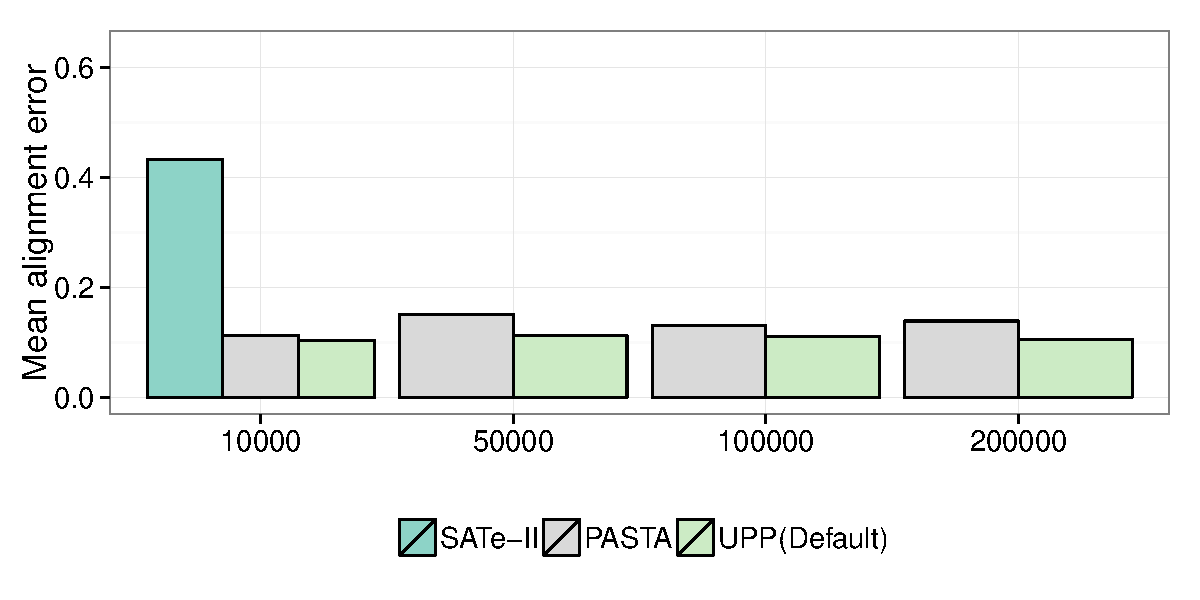
\includegraphics[width=0.70\linewidth]{{upp/rnasim.pasta.alignment_average}.pdf}\\
  \caption[]{Average alignment error}
\end{subfigure}
\begin{subfigure}[htpb]{\textwidth}
  \centering
  \includegraphics[width=0.70\linewidth]{{upp/rnasim.pasta.spfn}.pdf}\\
  \caption[]{Alignment SPFN error}
\end{subfigure}
\begin{subfigure}[htpb]{\textwidth}
  \centering
  \includegraphics[width=0.70\linewidth]{{upp/rnasim.pasta.spfp}.pdf}\\
  \caption[]{Alignment SPFP error}
\end{subfigure}
\caption[Alignment error of  PASTA, SAT\'e-II, and UPP for  
RNASim datasets.]{\label{rnasim_pasta_alignment}  {\bf Alignment error of UPP,
SAT\'e-II, and PASTA on the RNASim datasets.}  
UPP(Default) uses a backbone of size 1000. 
Results not shown indicate failure to complete within 24 hours using 12 processors.
}
\end{figure}

\begin{figure}[htpb]
\begin{subfigure}[htpb]{\textwidth}
  \centering
  \includegraphics[width=0.90\linewidth]{{upp/rnasim.pasta.fn}.pdf}\\
  \caption[]{FN tree error}
\end{subfigure}
\begin{subfigure}[htpb]{\textwidth}
  \centering
  \includegraphics[width=0.90\linewidth]{{upp/rnasim.pasta.delta_fn}.pdf}\\
  \caption[]{Delta FN tree error on the RNASim datasts.}
\end{subfigure}
\caption[Tree error  of PASTA, SAT\'e-II, and UPP for  
RNASim datasets.]{\label{rnasim_pasta_tree}  {\bf Tree error of  UPP,
SAT\'e-II,  and PASTA for the RNASim datasets.}  ML trees were estimated using FastTree under GTR.  UPP(Default) uses a backbone of size 1000.
Results not shown indicate failure to complete within 24 hours using 12 processors.}
\end{figure}

\begin{figure}[htpb]
\begin{subfigure}[htpb]{\textwidth}
  \centering
  \includegraphics[width=0.6\linewidth]{{upp/gutell.pasta.alignment_average}.pdf}\\
  \caption[]{Average alignment error}
\end{subfigure}
\begin{subfigure}[htpb]{\textwidth}
  \centering
  \includegraphics[width=0.6\linewidth]{{upp/gutell.pasta.spfn}.pdf}\\
  \caption[]{Alignment SPFN error}
\end{subfigure}
\begin{subfigure}[htpb]{\textwidth}
  \centering
  \includegraphics[width=0.6\linewidth]{{upp/gutell.pasta.spfp}.pdf}\\
  \caption[]{Alignment SPFP error}
\end{subfigure}
\caption[Alignment error of  PASTA, SAT\'e-II, and UPP on the
CRW datasets.]{\label{gutell_pasta_alignment}  {\bf Alignment error of  
SAT\'e-II, PASTA, and UPP on the CRW datasets.}  All methods were allowed to run till termination and were not limited by the 24 hour time limit.  UPP was run with 2 iterations on the 16S.T dataset.  UPP(Default) uses a backbone of size 1000.  Backbone sequences were selected from all sequences that were within 1500 bps $\pm$ 375 bps in length.}
%Nam - it would be good to have a figure showing results with one and two iterations.
\end{figure}

\begin{figure}[htpb]
\begin{subfigure}[htpb]{\textwidth}
  \centering
  \includegraphics[width=0.80\linewidth]{{upp/gutell.pasta.fn}.pdf}\\
  \caption[]{FN tree error}
\end{subfigure}
\begin{subfigure}[htpb]{\textwidth}
  \centering
  \includegraphics[width=0.80\linewidth]{{upp/gutell.pasta.delta_fn}.pdf}\\
  \caption[]{Delta FN tree error}
\end{subfigure}
\caption[Tree error rates for UPP, SAT\'e-II, and PASTA on the 
CRW datasets.]{\label{gutell_pasta_tree}  {\bf Tree error for PASTA, SAT\'e-II,
and UPP on the CRW datasets.}  
ML trees were estimated using FastTree under GTR.  All methods were allowed to run till termination and were not limited by the 24 hour time limit.  UPP was run with 2 iterations on the 16S.T dataset.  UPP(Default) uses a backbone of size 1000.  Backbone sequences were selected from all sequences that were within 1500 bps $\pm$ 375 bps in length.}
\end{figure}


\begin{figure}[htpb]
\begin{subfigure}[htpb]{\textwidth}
  \centering
  \includegraphics[width=0.6\linewidth]{{upp/fasttree.pasta.alignment_average}.pdf}\\
  \caption[]{Average alignment error}
\end{subfigure}
\begin{subfigure}[htpb]{\textwidth}
  \centering
  \includegraphics[width=0.6\linewidth]{{upp/fasttree.pasta.spfn}.pdf}\\
  \caption[]{Alignment SPFN error}
\end{subfigure}
\begin{subfigure}[htpb]{\textwidth}
  \centering
  \includegraphics[width=0.6\linewidth]{{upp/fasttree.pasta.spfp}.pdf}\\
  \caption[]{Alignment SPFP error}
\end{subfigure}
\caption[Alignment error of  PASTA and UPP on the
FastTree COG datasets.]{\label{fasttree_pasta_alignment}  {\bf Alignment error of PASTA and UPP on the FastTree COG datasets.}  Backbone sequences were filtered by only selecting from sequences within 75\% to 125\% in length of the median sequnce length of the reference sequences.  Standard error bars are shown.}
\end{figure}

\begin{figure}[htpb]
\begin{subfigure}[htpb]{\textwidth}
  \centering
  \includegraphics[width=0.90\linewidth]{{upp/fasttree.pasta.fn}.pdf}\\
  \caption[]{FN tree error}
\end{subfigure}
\begin{subfigure}[htpb]{\textwidth}
  \centering
  \includegraphics[width=0.90\linewidth]{{upp/fasttree.pasta.delta_fn}.pdf}\\
  \caption[]{Delta FN tree error}
\end{subfigure}
\caption[Tree error of  UPP and PASTA on the 
FastTree COG datasets.]{\label{fasttree_pasta_tree}  
%Nam - provide AA model
{\bf Tree error of UPP and PASTA on the simulated FastTree COG datasets.}  
ML trees were estimated using FastTree under JTT.  Backbone sequences were filtered by only selecting from sequences within 75\% to 125\% in length of the median sequnce length of the reference sequences.  UPP(Default) uses a backbone of size 1000.  Standard error bars are shown.  }
\end{figure}


\clearpage

\begin{figure}[htpb]
%\begin{subfigure}[htpb]{\textwidth}
  \centering
  \includegraphics[width=0.90\linewidth]{{upp/homfam.pasta.alignment_average}.pdf}\\
%  \caption[]{Average alignment error}
%\end{subfigure}
%\begin{subfigure}[htpb]{\textwidth}
%  \centering
%  \includegraphics[width=0.70\linewidth]{{upp/homfam.pasta.spfn}.pdf}\\
%  \caption[]{Alignment SPFN error}
%\end{subfigure}
%\begin{subfigure}[htpb]{\textwidth}
%  \centering
%  \includegraphics[width=0.70\linewidth]{{upp/homfam.pasta.spfp}.pdf}\\
%  \caption[]{Alignment SPFP error}
%\end{subfigure}
\caption[ Average alignment
error of  PASTA and UPP on
HomFam datasets.]{\label{homfam_pasta_alignment_mean}  
{\bf Average alignment error of UPP and PASTA on the HomFam datasets.}  UPP(Default) uses a backbone of size 1000. Backbone sequences were filtered by only selecting from sequences within 75\% to 125\% in length of the median sequnce length of the seed sequences.  Standard error bars are shown.}
\end{figure}
\clearpage

\begin{figure}[htpb]
%\begin{subfigure}[htpb]{\textwidth}
%  \centering
%  \includegraphics[width=0.70\linewidth]{{upp/homfam.pasta.alignment_average}.pdf}\\
%  \caption[]{Average alignment error}
%\end{subfigure}
\begin{subfigure}[htpb]{\textwidth}
  \centering
  \includegraphics[width=0.90\linewidth]{{upp/homfam.pasta.spfn}.pdf}\\
  \caption[]{Alignment SPFN error}
\end{subfigure}
\begin{subfigure}[htpb]{\textwidth}
  \centering
  \includegraphics[width=0.90\linewidth]{{upp/homfam.pasta.spfp}.pdf}\\
  \caption[]{Alignment SPFP error}
\end{subfigure}
\caption[SPFN and SPFP alignment
error of  PASTA and UPP on 
HomFam datasets.]{\label{homfam_pasta_alignment}  
{\bf SPFN and SPFP alignment error of UPP and PASTA on the HomFam datasets.}  
UPP(Default) uses a backbone of size 1000.  Backbone sequences were filtered by only selecting from sequences within 75\% to 125\% in length of the median sequnce length of the seed sequences.  Standard error bars are shown.}
\end{figure}

\begin{figure}[htpb]
\begin{subfigure}[htpb]{\textwidth}
  \centering
  \includegraphics[width=0.6\linewidth]{{upp/frag.1000M2.alignment_average.pasta.500}.pdf}\\
  \caption[]{Average alignment error}
\end{subfigure}
\begin{subfigure}[htpb]{\textwidth}
  \centering
  \includegraphics[width=0.6\linewidth]{{upp/frag.1000M2.spfn.pasta.500}.pdf}\\
  \caption[]{Alignment SPFN error}
\end{subfigure}
\begin{subfigure}[htpb]{\textwidth}
  \centering
  \includegraphics[width=0.6\linewidth]{{upp/frag.1000M2.spfp.pasta.500}.pdf}\\
  \caption[]{Alignment SPFP error}
\end{subfigure}
\caption[Alignment error of PASTA and UPP on  
the fragmentary 1000M2 datasets.]{\label{frag_1000M2_pasta_alignment}  {\bf Alignment error of PASTA and UPP on the fragmentary 1000M2 datasets.}  UPP(Default) uses a backbone size equal to the total number of full-length sequences.  Backbone sequences were filtered by only selecting from sequences within 75\% to 125\% length of the typical 1000M2 length (1000 bps).  Fragments had an average length of 500 bps, roughly one half the length of an average full length sequence from 1000M2.  Note that at 0\% fragmentation, UPP(Default)  is identical to PASTA.  Standard error bars are shown.  Averages are computed over 5 replicates per dataset.}
\end{figure}

\begin{figure}[htpb]
%\begin{subfigure}[htpb]{\textwidth}
  \centering
  \includegraphics[width=0.90\linewidth]{{upp/frag.1000M2.delta_fn.pasta.500}.pdf}\\
%  \caption[]{Delta FN tree error}
%\end{subfigure}
\caption[Delta FN tree error of UPP and PASTA on the fragmentary 1000M2 datasets.]{\label{frag_1000M2_pasta_tree}  {\bf Delta FN Tree error of UPP and PASTA on the fragmentary 1000M2 datasets.}  UPP(Default) uses a backbone size equal to the total number of full-length sequences.  Backbone sequences were filtered by only selecting from sequences within 75\% to 125\% length of the typical 1000M2 length (1000 bps).  ML trees were estimated using FastTree under GTR.  Fragments had an average length of 500 bps, roughly one half the length of an average full length sequence from 1000M2.  Note that at 0\% fragmentation, UPP(Default) is identical to PASTA.  Standard error bars are shown.  Averages are computed over 5 replicates per dataset.}
\end{figure}

\clearpage
% \subsection{UPP versus SEPP}\label{sec:som-upp-vs-sepp}
% We present results comparing UPP and SEPP.  In general, the alignment accuracy of UPP and SEPP tend to be comparable (Figs.~\ref{rnasim_sepp_alignment},~\ref{gutell_sepp_alignment}, and ~\ref{small_frag_sepp}), but on datasets where there are differences in alignment accuracy , they tend to favor UPP (Figure ~\ref{large_frag_sepp}).  With respec to tree accuracy, we see much larger differences.  UPP tends to result in much more accurate trees than SEPP (~\ref{large_frag_sepp}).

% \textbf{Finish tree estimation on datasets, add in actual numbers}
% \begin{figure}[htpb]
% \begin{subfigure}[htpb]{\textwidth}
  % \centering
  % \includegraphics[width=0.70\linewidth]{{upp/rnasim.sepp.alignment_average}.pdf}\\
  % \caption[]{Average alignment error}
% \end{subfigure}
% \begin{subfigure}[htpb]{\textwidth}
  % \centering
  % \includegraphics[width=0.70\linewidth]{{upp/rnasim.sepp.spfn}.pdf}\\
  % \caption[]{Alignment SPFN error}
% \end{subfigure}
% \begin{subfigure}[htpb]{\textwidth}
  % \centering
  % \includegraphics[width=0.70\linewidth]{{upp/rnasim.sepp.spfp}.pdf}\\
  % \caption[]{Alignment SPFP error}
% \end{subfigure}
% \caption[Alignment error of UPP variants for  
% RNASim datasets.]{\label{rnasim_sepp_alignment}  {\bf Alignment
% error for UPP versus SEPP on the RNASim datasets.}  UPP and SEPP ``default'' use a backbone of size 1000.  UPP and SEPP ``fast'' use a backbone of size 100.}
% \end{figure}

% \begin{figure}[htpb]
% \begin{subfigure}[htpb]{\textwidth}
  % \centering
  % \includegraphics[width=0.90\linewidth]{{upp/rnasim.sepp.fn}.pdf}\\
  % \caption[]{FN tree error}
% \end{subfigure}
% \begin{subfigure}[htpb]{\textwidth}
  % \centering
  % \includegraphics[width=0.90\linewidth]{{upp/rnasim.sepp.delta_fn}.pdf}\\
  % \caption[]{Delta FN tree error}
% \end{subfigure}
% \caption[Tree error for UPP versus SEPP on  
% RNASim datasets.]{\label{rnasim_sepp_tree}  {\bf Tree error UPP versus SEPP on the RNASim datasets.}  ML trees were estimated using FastTree.  UPP and SEPP ``default'' use a backbone of size 1000.  UPP and SEPP ``fast'' use a backbone of size 100.}
% \end{figure}

% \begin{figure}[htpb]
% \centering
% \includegraphics[width=0.90\linewidth]{{upp/rnasim.sepp.wall_align_time}.pdf}\\
% \caption[Wall clock alignment time (hrs) for UPP versus SEPP on  
% RNASim datasets.]{\label{rnasim_sepp_time}  {\bf  Wall clock alignment time (hrs) of UPP versus SEPP on the RNASim datasets.}  
% All methods were run on a machine with 12 CPUs and 24 GB of memory.  UPP and SEPP ``default'' use a backbone of size 1000.  UPP and SEPP ``fast'' use a backbone of size 100.}
% \end{figure}


% \begin{figure}[htpb]
% \begin{subfigure}[htpb]{\textwidth}
  % \centering
  % \includegraphics[width=0.55\linewidth]{{upp/gutell.sepp.alignment_average}.pdf}\\
  % \caption[]{Average alignment error}
% \end{subfigure}
% \begin{subfigure}[htpb]{\textwidth}
  % \centering
  % \includegraphics[width=0.55\linewidth]{{upp/gutell.sepp.spfn}.pdf}\\
  % \caption[]{Alignment SPFN error}
% \end{subfigure}
% \begin{subfigure}[htpb]{\textwidth}
  % \centering
  % \includegraphics[width=0.55\linewidth]{{upp/gutell.sepp.spfp}.pdf}\\
  % \caption[]{Alignment SPFP error}
% \end{subfigure}
% \caption[Alignment error for UPP versus SEPP on  
% Gutell datasets.]{\label{gutell_sepp_alignment}  {\bf Alignment
% error for UPP versus SEPP on the Gutell datasets.}  UPP and SEPP ``default'' use a backbone of size 1000.  UPP and SEPP ``fast'' use a backbone of size 100.  Backbone sequences were selected from all sequences that were within 1500 bps $\pm$ 375 bps in length.  UPP(Default,No Decomp) and UPP(Fast,No Decomp) failed to align one sequence on the 16S.T. dataset, and thus, results for these methods on 16S.T are not shown.  \textbf{Add in results as they complete for Gutell.}}
% \end{figure}

% \begin{figure}[htpb]
% \begin{subfigure}[htpb]{\textwidth}
  % \centering
  % \includegraphics[width=0.90\linewidth]{{upp/gutell.sepp.fn}.pdf}\\
  % \caption[]{FN tree error}
% \end{subfigure}
% \begin{subfigure}[htpb]{\textwidth}
  % \centering
  % \includegraphics[width=0.90\linewidth]{{upp/gutell.sepp.delta_fn}.pdf}\\
  % \caption[]{Delta FN tree error}
% \end{subfigure}
% \caption[Tree error for UPP versus SEPP on the
% Gutell datasets.]{\label{gutell_sepp_tree}  {\bf Tree error for UPP versus SEPP on the Gutell datasets.}  
% ML trees were estimated using FastTree.  
% UPP and SEPP ``default'' use a backbone of size 1000.  UPP and SEPP ``fast'' use a backbone of size 100.  Backbone sequences were selected from all sequences that were within 1500 bps $\pm$ 375 bps in length.  UPP(Default,No Decomp) and UPP(Fast,No Decomp) failed to align one sequence on the 16S.T. dataset, and thus, results for these methods on 16S.T are not shown. \textbf{Trees need to finish estimating on Gutell.}}
% \end{figure}

% \begin{figure}[htpb]
% \centering
% \includegraphics[width=0.90\linewidth]{{upp/gutell.sepp.wall_align_time}.pdf}\\
% \caption[Wall clock alignment time (hrs) for UPP versus SEPP on  
% Gutell datasets.]{\label{gutell_sepp_time}  {\bf Wall clock alignment time (hrs) for UPP versus SEPP on the Gutell datasets.}  
% All methods were run on a machine with 12 CPUs and 24 GB of memory.  UPP and SEPP ``default'' use a backbone of size 1000.  UPP and SEPP ``fast'' use a backbone of size 100.  Backbone sequences were selected from all sequences that were within 1500 bps $\pm$ 375 bps in length.  UPP(Default,No Decomp) and UPP(Fast,No Decomp) failed to align one sequence on the 16S.T. dataset, and thus, results for these methods on 16S.T are not shown. \textbf{Add in results as they complete.}}
% \end{figure}

% \begin{figure}[htpb]
% \begin{subfigure}[htpb]{\textwidth}
  % \centering
  % \includegraphics[width=0.9\linewidth]{{upp/1000_taxa_fragments_alignment_mean.sepp}.pdf}\\
  % \caption[]{Average alignment error}
% \end{subfigure}
% \begin{subfigure}[htpb]{\textwidth}
  % \centering
  % \includegraphics[width=0.9\linewidth]{{upp/1000_taxa_fragments_delta_fn.sepp}.pdf}\\
  % \caption[]{Delta tree error}
% \end{subfigure}
% \caption[Results of MAFFT variants on 
% fragmentary
% 1000-taxon datasets.]{\label{small_frag_sepp}  
% {\bf Results of UPP versus SEPP on the fragmentary 1000-taxon datasets.}  All ML trees were estimated using FastTree.  Fragmentary sequences were simulated with an average fragment length of 500 bps (i.e., half length).  Backbone sequences were selected from all sequences that were within 1000 bps $\pm$ 250 bps in length.  Standard error bars are shown.  Averages are computed over 5 replicates per dataset.}  
% \end{figure}

% \begin{figure}[htpb]
% \begin{subfigure}[htpb]{\textwidth}
  % \centering
  % \includegraphics[width=0.9\linewidth]{{upp/large_fragments_alignment_mean.sepp}.pdf}\\
  % \caption[]{Average alignment error}
% \end{subfigure}
% \begin{subfigure}[htpb]{\textwidth}
  % \centering
  % \includegraphics[width=0.9\linewidth]{{upp/large_fragments_delta_fn.sepp}.pdf}\\
  % \caption[]{Delta tree error}
% \end{subfigure}
% \caption[Results of UPP versus SEPP on the large
% fragmentary datasets.]{\label{large_frag_sepp}  
% {\bf Results of UPP versus SEPP on the large fragmentary datasets.}  All ML trees were estimated using FastTree.  Fragmentary sequences were simulated with an average fragment length of 500 bps (i.e., half length).  Backbone sequences were selected from all sequences that were within 1000 bps $\pm$ 250 bps in length.  Standard error bars are shown.}  
% \end{figure}

\clearpage 
\subsection{Backbone and final alignment error.}\label{backbone_alignment_error}
We examined the alignment error of the backbone alignment and the resulting alignment error 
of the alignment generated by UPP using the HMM Family technique, or using
MAFFT-profile ``add'' or MAFFT-profile ``addfragments'' (Fig.~\ref{backbone_error}).

We found that the backbone alignment error was statistically significantly correlated to the alignments generated by the UPP pipeline (Pearson's correlation coefficient 0.897; p-value of 2.292e-10). We also found that alignment errors on alignments generated by the HMM Family
technique (UPP(Default)) were closer to the original backbone alignment error 
than when they were generated using 
MAFFT-profile (root mean squared difference in alignment error of 0.020 for UPP(Default) 
versus 0.024 and 0.051 for UPP using MAFFT-profile ``addfragments'' and 
MAFFT-profile ``add'', respectively).

This result shows that the HMM Family technique best preserves the alignment accuracy of the original backbone alignment and can be used as a way to scale existing alignments methods to ultra-large datasets.  

\begin{figure}[htpb]
  \centering
  \includegraphics[width=0.850\linewidth]{{upp/backbone_alignment}.pdf}\\
\caption[Comparison of initial backbone alignment error and final UPP alignment error.]
{\label{backbone_error}  {\bf Comparison of initial backbone error and final 
UPP alignment error,  using PASTA backbones of size 1000.}  
 Each point represents the alignment error for a specific method on a specific dataset.  Points below the line represent alignment methods that have a lower alignment error relative to the backbone alignment.  Points above the line represent alignment methods that have a higher alignment error relative to the backbone alignment.  The Pearson's correlation coefficient for the backbone alignment error versus the final alignment error for the entire collection of points is 0.897 and is statistically significantly correlated (p-value of 2.292e-10; Pearson's product-moment correlation test).}
%Nam - do we have this for small backbones?
%Tandy:  We only have it for RNASim, which adding would
%clutter the results, as it adds 3 methods with 1 datapoint each
\end{figure}

% \begin{figure}[htpb]
% \centering
% \includegraphics[width=1.10\linewidth]{{upp/backbone_methods}.pdf}\\
% \caption[Initial backbone error versus final alignment error.]{\label{backbone_error_alignment}  {\bf Initial backbone alignment error versus UPP(Fast) final alignment error for the RNASim 10K dataset.}  Results for one replicate of the RNASim 10K dataset.  A backbone set of 100 were randomly sampled, and PASTA, Clustal-Omega, MUSCLE, and MAFFT-L-INS-i backbone alignments were estimated on the backbone set.  UPP(Fast) was run on each backbone alignment and the alignment error of the backbone alignment and the final UPP(Fast) alignment are reported.}
% \end{figure}

\clearpage


%Compute correlation co-efficients
\clearpage
\subsection{Results on full-length datasets}\label{sec:all_methods}
We present results on all the full-length sequence datasets.

\begin{figure}[htpb]
\begin{subfigure}[htpb]{\textwidth}
  \centering
  \includegraphics[width=0.70\linewidth]{{upp/rnasim.main.alignment_average}.pdf}\\
  \caption[]{Average alignment error}
\end{subfigure}
\begin{subfigure}[htpb]{\textwidth}
  \centering
  \includegraphics[width=0.70\linewidth]{{upp/rnasim.main.spfn}.pdf}\\
  \caption[]{Alignment SPFN error}
\end{subfigure}
\begin{subfigure}[htpb]{\textwidth}
  \centering
  \includegraphics[width=0.70\linewidth]{{upp/rnasim.main.spfp}.pdf}\\
  \caption[]{Alignment SPFP error}
\end{subfigure}
\caption[Alignment error on
the
RNASim datasets.]{\label{rnasim_all_alignment}  {Alignment error on the RNASim datasets.}  MAFFT is run under the default options on the RNASim 10K and 50K datasets and under ``PartTree'' for the RNASim 100K dataset.  UPP(Fast) use a backbone size of 100.}
%Nam - how is MAFFT run?
\end{figure}

\clearpage

\begin{figure}[htpb]
\begin{subfigure}[htpb]{\textwidth}
  \centering
  \includegraphics[width=0.90\linewidth]{{upp/rnasim.main.fn}.pdf}\\
  \caption[]{FN tree error}
\end{subfigure}
\begin{subfigure}[htpb]{\textwidth}
  \centering
  \includegraphics[width=0.90\linewidth]{{upp/rnasim.main.delta_fn}.pdf}\\
  \caption[]{Delta FN tree error}
\end{subfigure}
\caption[Tree error  on the
RNASim datasets.]{\label{rnasim_all_tree}  {\bf Tree error on the RNASim datasets.}  
ML trees were estimated using FastTree under GTR.  MAFFT is run under the default options on the RNASim 10K and 50K datasets and under ``PartTree'' for the RNASim 100K dataset.  UPP(Fast)  use a backbone size of 100.}
%Nam - how is MAFFT run?
\end{figure}

\begin{figure}[htpb]
\centering
\includegraphics[width=0.90\linewidth]{{upp/rnasim.main.wall_align_time}.pdf}\\
\caption[Wall clock alignment time (hrs) on the
RNASim datasets.]{\label{rnasim_all_time}  {\bf Wall clock alignment time (hrs) on the RNASim datasets.}  
All methods were run on a machine with 12 CPUs and 24 GB of memory.  MAFFT is run under the default options on the RNASim 10K and 50K datasets and under ``PartTree'' for the RNASim 100K dataset;
the difference in how MAFFT was run explains the diffrence in time
between 50K and 100K sequences.  UPP(Fast) uses a backbone size of 100.}
%Nam - how is MAFFT run?
\end{figure}

\clearpage

\begin{figure}[htpb]
%\begin{subfigure}[htpb]{\textwidth}
  \centering
  \includegraphics[width=0.90\linewidth]{{upp/1000_taxa.main.alignment_average.hard}.pdf}\\
%  \caption[]{Average alignment error}
%\end{subfigure}
%\begin{subfigure}[htpb]{\textwidth}
%  \centering
%  \includegraphics[width=0.70\linewidth]{{upp/1000_taxa.main.spfn.hard}.pdf}\\
%  \caption[]{Alignment SPFN error}
%\end{subfigure}
%\begin{subfigure}[htpb]{\textwidth}
%  \centering
%  \includegraphics[width=0.70\linewidth]{{upp/1000_taxa.main.spfp.hard}.pdf}\\
%  \caption[]{Alignment SPFP error}
%\end{subfigure}
\caption[Average  alignment error of different methods on the hardest 1000-taxon datasets.]
{\label{1000_taxon_main_alignment}  {\bf Average alignment
error of  different methods on the hardest 1000-taxon datasets.}  
Standard error bars are shown.  Averages are computed over 20 replicates per dataset.  UPP(Default) is identical to PASTA on these datasets.  }
%Nam - removed "Harmonic"
\end{figure}

\clearpage


\begin{figure}[htpb]
%\begin{subfigure}[htpb]{\textwidth}
%  \centering
%  \includegraphics[width=0.70\linewidth]{{upp/1000_taxa.main.alignment_average.hard}.pdf}\\
%  \caption[]{Average alignment error}
%\end{subfigure}
\begin{subfigure}[htpb]{\textwidth}
  \centering
  \includegraphics[width=0.90\linewidth]{{upp/1000_taxa.main.spfn.hard}.pdf}\\
  \caption[]{Alignment SPFN error}
\end{subfigure}
\begin{subfigure}[htpb]{\textwidth}
  \centering
  \includegraphics[width=0.90\linewidth]{{upp/1000_taxa.main.spfp.hard}.pdf}\\
  \caption[]{Alignment SPFP error}
\end{subfigure}
\caption[SPFN and SPFP alignment error of different methods on the hardest 1000-taxon datasets.]
{\label{1000_taxon_main_spfn_spfp}  {\bf SPFN and SPFP alignment
error of  different methods on the hardest 1000-taxon datasets.}  Standard error bars are shown.  Averages are computed over 20 replicates per dataset.  UPP(Default) is identical to PASTA on these datasets.  
}
\end{figure}


\begin{figure}[htpb]
\begin{subfigure}[htpb]{\textwidth}
  \centering
  \includegraphics[width=0.90\linewidth]{{upp/1000_taxa.main.fn.hard}.pdf}\\
  \caption[]{FN tree error}
\end{subfigure}
\begin{subfigure}[htpb]{\textwidth}
  \centering
  \includegraphics[width=0.90\linewidth]{{upp/1000_taxa.main.delta_fn.hard}.pdf}\\
  \caption[]{Delta FN tree error}
\end{subfigure}
\caption[Tree error of different methods on the hardest 1000-taxon datasets.]{\label{1000_taxon_main_tree}   {\bf Tree
error of different methods on  the hardest 1000-taxon datasets.} ML trees were estimated using FastTree under GTR.  Standard error bars are shown.  Averages are computed over 20 replicates per dataset.  UPP(Default) is identical to PASTA on these datasets.  }
\end{figure}


\begin{figure}[htpb]
%\begin{subfigure}[htpb]{\textwidth}
  \centering
  \includegraphics[width=0.90\linewidth]{{upp/indelible.main.alignment_average}.pdf}\\
%  \caption[]{Average alignment error}
%\end{subfigure}
%\begin{subfigure}[htpb]{\textwidth}
%  \centering
%  \includegraphics[width=0.60\linewidth]{{upp/indelible.main.spfn}.pdf}\\
%  \caption[]{Alignment SPFN error}
%\end{subfigure}
%\begin{subfigure}[htpb]{\textwidth}
%  \centering
%  \includegraphics[width=0.60\linewidth]{{upp/indelible.main.spfp}.pdf}\\
%  \caption[]{Alignment SPFP error}
%\end{subfigure}
\caption[Average alignment error on the Indelible datasets.]{\label{indelible_main_alignment}
{\bf Average  alignment error on the Indelible datasets.}  Clustal-Omega was unable to generate an alignment on the 10000M2 dataset (terminated with error message).  MAFFT was run under the default options.  Standard error bars are shown.  Averages are computed over 10 replicates per model condition.}
\end{figure}
%Nam - is this empty?

\clearpage
\begin{figure}[htpb]
%\begin{subfigure}[htpb]{\textwidth}
%  \centering
%  \includegraphics[width=0.60\linewidth]{{upp/indelible.main.alignment_average}.pdf}\\
%  \caption[]{Average alignment error}
%\end{subfigure}
\begin{subfigure}[htpb]{\textwidth}
  \centering
  \includegraphics[width=0.90\linewidth]{{upp/indelible.main.spfn}.pdf}\\
  \caption[]{Alignment SPFN error}
\end{subfigure}
\begin{subfigure}[htpb]{\textwidth}
  \centering
  \includegraphics[width=0.90\linewidth]{{upp/indelible.main.spfp}.pdf}\\
  \caption[]{Alignment SPFP error}
\end{subfigure}
\caption[SPFN and SPFP alignment error on the Indelible datasets.]{\label{indelible_spfn_spfp_alignment}  
{\bf SPFN and SPFP alignment error on the Indelible datasets.}  Clustal-Omega was unable to generate an alignment on the 10000M2 dataset (terminated with error message).  MAFFT was run under the default options.  Standard error bars are shown.  Averages are computed over 10 replicates per model condition.}
\end{figure}
\clearpage

\begin{figure}[htpb]
\begin{subfigure}[htpb]{\textwidth}
  \centering
  \includegraphics[width=0.90\linewidth]{{upp/indelible.main.fn}.pdf}\\
  \caption[]{FN tree error}
\end{subfigure}
\begin{subfigure}[htpb]{\textwidth}
  \centering
  \includegraphics[width=0.90\linewidth]{{upp/indelible.main.delta}.pdf}\\
  \caption[]{Delta FN tree error}
\end{subfigure}
\caption[Tree error rates on the Indelible datasets.]{\label{indelible_main_tree}
{\bf   Tree error on the Indelible datasets.}  Clustal-Omega was unable to generate an alignment on the 10000M2 dataset (terminated with error message).  MAFFT was run under the default options.  Standard error bars are shown.  Averages are computed over 10 replicates per model condition.}
\end{figure}

\begin{figure}[htpb]
  \centering
  \includegraphics[width=0.95\linewidth]{{upp/homfam.main.alignment_average}.pdf}\\
%  \caption[]{Average alignment error}
\caption[Average alignment error on the HomFam datasets.]{\label{homfam_main_alignment}
{\bf Average alignment error on the HomFam datasets.}
On the two largest HomFam datasets (zf-CCHH and rvp), MUSCLE terminated with a ``segfault'' error and was unable to produce an alignment.  Thus, average alignment error for MUSCLE is excluded from the results.  MAFFT is run under the default options.}
%{\bf Nam - but MUSCLE has a result under "average".
%Also, can you report just the average of SPFN and SPFP? 
%Tandy: MUSCLE result fixed
%Nam - looks like MUSCLE still shows up. (March 6) - please fix
\end{figure}


\clearpage

\begin{figure}[htpb]
%\begin{subfigure}[htpb]{\textwidth}
%  \centering
%  \includegraphics[width=0.60\linewidth]{{upp/homfam.main.alignment_average}.pdf}\\
%  \caption[]{Average alignment error}
%\end{subfigure}
\begin{subfigure}[htpb]{\textwidth}
  \centering
  \includegraphics[width=0.90\linewidth]{{upp/homfam.main.spfn}.pdf}\\
  \caption[]{Alignment SPFN error}
\end{subfigure}
\begin{subfigure}[htpb]{\textwidth}
  \centering
  \includegraphics[width=0.90\linewidth]{{upp/homfam.main.spfp}.pdf}\\
  \caption[]{Alignment SPFP error}
\end{subfigure}
\caption[Alignment SPFN and SPFP errors on the HomFam datasets.]{\label{homfam_main_spfn_spfp}  
{\bf Alignment SPFN and SPFP error on the HomFam datasets.}  
On the two largest HomFam datasets (zf-CCHH and rvp), MUSCLE terminated with a ``segfault'' error and was unable to produce an alignment.  Thus, average alignment error for MUSCLE is excluded from the results.  MAFFT is run under the default options.}
%Nam - looks like MUSCLE still shows up. (March 6)
\end{figure}


\begin{figure}[htpb]
%\begin{subfigure}[htpb]{\textwidth}
  \centering
  \includegraphics[width=0.90\linewidth]{{upp/balibase.main.alignment_average}.pdf}\\
  %\caption[]{Average alignment error}
%\end{subfigure}
% \begin{subfigure}[htpb]{\textwidth}
  % \centering
  % \includegraphics[width=0.60\linewidth]{{upp/balibase.main.spfn}.pdf}\\
  % \caption[]{Alignment SPFN error}
% \end{subfigure}
% \begin{subfigure}[htpb]{\textwidth}
  % \centering
  % \includegraphics[width=0.60\linewidth]{{upp/balibase.main.spfp}.pdf}\\
  % \caption[]{Alignment SPFP error}
% \end{subfigure}
\caption[Average alignment error on the ten
large protein datasets with full alignments.]{\label{balibase_main_alignment_mean}  
{\bf Average alignment errors on the ten large protein datasets with full alignments.}  MAFFT is run under ``L-INS-I''}
\end{figure}

\begin{figure}[htpb]
% \begin{subfigure}[htpb]{\textwidth}
  % \centering
  % \includegraphics[width=0.60\linewidth]{{upp/balibase.main.alignment_average}.pdf}\\
  % \caption[]{Average alignment error}
% \end{subfigure}
\begin{subfigure}[htpb]{\textwidth}
  \centering
  \includegraphics[width=0.85\linewidth]{{upp/balibase.main.spfn}.pdf}\\
  \caption[]{Alignment SPFN error}
\end{subfigure}
\begin{subfigure}[htpb]{\textwidth}
  \centering
  \includegraphics[width=0.85\linewidth]{{upp/balibase.main.spfp}.pdf}\\
  \caption[]{Alignment SPFP error}
\end{subfigure}
\caption[SPFN and SPFP alignment error rates on the ten
large protein datasets with full alignments.]{\label{balibase_main_alignment_sop}  
{\bf Alignment SPFN and SPFP error on the ten large protein datasets with full alignments.}  MAFFT is run under ``L-INS-I''}
%Nam - see if these results match Keerthana's results ...
%KK's clustal-omega is slightly worse alignment, but overall, the results are very close
\end{figure}

\begin{figure}[htpb]
\begin{subfigure}[htpb]{\textwidth}
  \centering
  \includegraphics[width=0.90\linewidth]{{upp/balibase.main.fn}.pdf}\\
%  \caption[]{FN tree error}
\end{subfigure}
\caption[RAxML tree error rates on the ten large 
protein datasets with full alignments, under the JTT model.]{\label{balibase_main_tree}  
{\bf Tree error rates on the large protein datasets with
full alignments}. MAFFT is run under ``L-INS-I''.
ML trees were estimated using RAxML under JTT.}
%Nam - see if these results match Keerthana's results...
%These results are very close, but it's difficult to really compare
%because KK used different models
\end{figure}

\clearpage
\begin{figure}[htpb]
%\begin{subfigure}[htpb]{\textwidth}
  \centering
  \includegraphics[width=0.90\linewidth]{{upp/fasttree.main.alignment_average}.pdf}\\
%  \caption[]{Average alignment error}
%\end{subfigure}
%\begin{subfigure}[htpb]{\textwidth}
%  \centering
%  \includegraphics[width=0.60\linewidth]{{upp/fasttree.main.spfn}.pdf}\\
%  \caption[]{Alignment SPFN error}
%\end{subfigure}
%\begin{subfigure}[htpb]{\textwidth}
%  \centering
%  \includegraphics[width=0.60\linewidth]{{upp/fasttree.main.spfp}.pdf}\\
%  \caption[]{Alignment SPFP error}
%\end{subfigure}
\caption[Average alignment error on the FastTree COG datasets.]{\label{fasttree_main_alignment_average}  
{\bf Average alignment error on the FastTree COG datasets.}   MAFFT is run under the default options.  Opal failed to generate an alignment on COG438, and thus is excluded from the average results.}
\end{figure}


\begin{figure}[htpb]
%\begin{subfigure}[htpb]{\textwidth}
%  \centering
%  \includegraphics[width=0.60\linewidth]{{upp/fasttree.main.alignment_average}.pdf}\\
%  \caption[]{Average alignment error}
%\end{subfigure}
\begin{subfigure}[htpb]{\textwidth}
  \centering
  \includegraphics[width=0.90\linewidth]{{upp/fasttree.main.spfn}.pdf}\\
  \caption[]{Alignment SPFN error}
\end{subfigure}
\begin{subfigure}[htpb]{\textwidth}
  \centering
  \includegraphics[width=0.90\linewidth]{{upp/fasttree.main.spfp}.pdf}\\
  \caption[]{Alignment SPFP error}
\end{subfigure}
\caption[SPFN and SPFP alignment error on the FastTree COG datasets.]{\label{fasttree_spfn_spfp_alignment}  
{\bf SPFN and SPFP alignment error on the simulated FastTree COG datasets.} MAFFT is run under the default options.  Opal failed to generate an alignment on COG438, and thus is excluded from the average results.
}
\end{figure}

\begin{figure}[htpb]
\begin{subfigure}[htpb]{\textwidth}
  \centering
  \includegraphics[width=0.90\linewidth]{{upp/fasttree.main.fn}.pdf}\\
  \caption[]{FN tree error}
\end{subfigure}
\begin{subfigure}[htpb]{\textwidth}
  \centering
  \includegraphics[width=0.90\linewidth]{{upp/fasttree.main.delta_fn}.pdf}\\
  \caption[]{Delta FN tree error}
\end{subfigure}
\caption[Tree error rates on the FastTree COG datasets.]
{\label{fasttree_main_tree}{\bf  
Tree error rates on the simulated FastTree COG datasets.}  
ML trees were estimated using FastTree under JTT. MAFFT is run under the default options.  Opal failed to generate an alignment on COG438, and thus is excluded from the average results.}
\end{figure}

\begin{figure}[htpb]
\begin{subfigure}[htpb]{\textwidth}
  \centering
  \includegraphics[width=0.60\linewidth]{{upp/gutell.main.alignment_average}.pdf}\\
  \caption[]{Average alignment error}
\end{subfigure}
\begin{subfigure}[htpb]{\textwidth}
  \centering
  \includegraphics[width=0.60\linewidth]{{upp/gutell.main.spfn}.pdf}\\
  \caption[]{Alignment SPFN error}
\end{subfigure}
\begin{subfigure}[htpb]{\textwidth}
  \centering
  \includegraphics[width=0.60\linewidth]{{upp/gutell.main.spfp}.pdf}\\
  \caption[]{Alignment SPFP error}
\end{subfigure}
\caption[Alignment error rates on the CRW datasets.]{\label{gutell_main_alignment}  {\bf Alignment error
rates  on the CRW datasets.}  MAFFT is run under the default options on the 16S.T and 16S.3 datasets and under ``PartTree'' on the 16S.B.ALL dataset.  UPP results are based on the first iteration of UPP.
%Nam - probably we need to show this with 
%second iteration.
%These are the individual results for the main paper, as such, we limit those results to 24 hours of running time.
}
\end{figure}

%\begin{figure}[htpb]
%\begin{subfigure}[htpb]{\textwidth}
%  \centering
%  \includegraphics[width=0.90\linewidth]{{upp/gutell.main.fn}.pdf}\\
%  \caption[]{FN tree error}
%\end{subfigure}
%\begin{subfigure}[htpb]{\textwidth}
%  \centering
%  \includegraphics[width=0.90\linewidth]{{upp/gutell.main.delta_fn}.pdf}\\
%  \caption[]{Delta FN tree error}
%\end{subfigure}
%\caption[Results comparing tree error rates on the Gutell CRW datasets.]{\label{gutell_main_tree}{\bf  Tree error rates on the Gutell CRW datasets.}  ML trees were estimated using FastTree under GTR. MAFFT is run under the default options on the 16S.T and 16S.3 datasets and under ``PartTree'' on the 16S.B.ALL dataset.  
%UPP results shown are based on the first iteration of UPP.
%%Nam, probably we need to show this with second iteration.
%I commented it out because I think we need to show this with 2 iterations.
%}
%\end{figure}


\clearpage
\subsection{TC Scores}
\label{SOM:sec-TC}
We report total column (TC) scores on the protein datasets with structurally based reference alignments (Fig.~\ref{all_tc_score}).  The TC score is the proportion of columns
in the reference alignment that are recovered in the estimated alignment.  
%TC scores can be useful for scoring the quality of structurally-based alignments, with the idea that the structures are well conserved.  

UPP, MAFFT, and Clustal-Omega have similar TC scores on the ten large AA datasets, followed closely by Opal and Muscle.  On the HomFam datasets, the differences between the methods are more clear with UPP having the best TC score, followed by MAFFT, then Clustal-Omega.

\begin{figure}[htpb]
\begin{subfigure}[htpb]{\textwidth}
  \centering
  \includegraphics[width=0.90\linewidth]{{upp/balibase.main.tc}.pdf}\\
  \caption[]{TC scores on the ten large biological datasets with full alignments}
\end{subfigure}
\begin{subfigure}[htpb]{\textwidth}
  \centering
  \includegraphics[width=0.90\linewidth]{{upp/homfam.main.tc}.pdf}\\
  \caption[]{TC scores on the Homfam datasets }
\end{subfigure}
\caption[TC scores on the biological
AA datasets ]{\label{all_tc_score}  {\bf TC (Total Column) scores of methods on the 
biological AA datasets.}  MAFFT is run under ``L-INS-i'' option on the ten large AA datasets and under the default option on the HomFam datasets.}
\end{figure}


\clearpage
\subsection{Results on fragmentary datasets}\label{sec:all_frag_methods}
We present results on the individual fragmentary datasets.  

\begin{figure}[htpb]
\begin{subfigure}[htpb]{\textwidth}
  \centering
  \includegraphics[width=0.55\linewidth]{{upp/1000_taxa_fragments_alignment_average.main}.pdf}\\
  \caption[]{Average alignment error}
\end{subfigure}
\begin{subfigure}[htpb]{\textwidth}
  \centering
  \includegraphics[width=0.55\linewidth]{{upp/1000_taxa_fragments_spfn.main}.pdf}\\
  \caption[]{Alignment SPFN error}
\end{subfigure}
\begin{subfigure}[htpb]{\textwidth}
  \centering
  \includegraphics[width=0.55\linewidth]{{upp/1000_taxa_fragments_spfp.main}.pdf}\\
  \caption[]{Alignment SPFP error}
\end{subfigure}
\caption[Alignment error rates on the fragmentary 1000-taxon datasets.]{\label{fragmentary_1000_taxa_alignment}  {\bf Alignment error rates on the fragmentary 1000-taxon model conditions.} We show alignment error rates for different methods on the 
 1000M2, 1000M3, and 1000M4 datasets, varying 
the percentage of fragmentary sequences, each with an average 
length of 500 sites 
(i.e., approximately half the average sequence length). MAFFT is run under the ``L-INS-i''.  Standard error bars are shown.  Averages are computed over 5 replicates per dataset.}
\end{figure}

\begin{figure}[htpb]
\begin{subfigure}[htpb]{\textwidth}
  \centering
  \includegraphics[width=0.85\linewidth]{{upp/1000_taxa_fragments_fn.main}.pdf}\\
  \caption[]{FN tree error}
\end{subfigure}
\begin{subfigure}[htpb]{\textwidth}
  \centering
  \includegraphics[width=0.85\linewidth]{{upp/1000_taxa_fragments_delta_fn.main}.pdf}\\
  \caption[]{Delta FN tree error}
\end{subfigure}
\caption[Tree error rates on the fragmentary 1000-taxon datasets.]{\label{fragmentary_1000_taxa_tree}{\bf  Tree error rates on the fragmentary 1000-taxon  datasets.}  We show tree error rates for different methods on the 
 1000M2, 1000M3, and 1000M4 datasets, varying 
the percentage of fragmentary sequences, each with an average 
length of 500 sites 
(i.e., approximately half the average sequence length).  MAFFT is run under the ``L-INS-i''.  ML trees were estimated using FastTree under GTR.  Standard error bars are shown.  Averages are computed over 5 replicates per dataset.}
\end{figure}

% \begin{figure}[htpb]
% \begin{subfigure}[htpb]{\textwidth}
  % \centering
  % \includegraphics[width=0.65\linewidth]{{upp/large_fragmentary.gutell.alignment_mean.main}.pdf}\\
  % \caption[]{Average alignment error}
% \end{subfigure}
% \begin{subfigure}[htpb]{\textwidth}
  % \centering
  % \includegraphics[width=0.65\linewidth]{{upp/large_fragmentary.gutell.spfn.main}.pdf}\\
  % \caption[]{Alignment SPFN error}
% \end{subfigure}
% \begin{subfigure}[htpb]{\textwidth}
  % \centering
  % \includegraphics[width=0.65\linewidth]{{upp/large_fragmentary.gutell.spfp.main}.pdf}\\
  % \caption[]{Alignment SPFP error}
% \end{subfigure}
% \caption[Alignment error rates on the fragmentary CRW 16S.T and 16S.3 datasets.]{\label{fragmentary_gutell_alignment}  {\bf Alignment error rates on the fragmentary CRW 16S.T and 16S.3 datasets.} We show alignment error rates for 
% Clustal-Omega, MUSCLE, MAFFT-Default, and UPP
% on the 
% CRW 16S.T and 16S.3 datasets, varying 
% the percentage of fragmentary sequences, each with an average 
% length of 500 sites 
% (i.e., approximately one third the average sequence length).  UPP results shown are based on the first iteration of UPP. 
% }
% \end{figure}

% \begin{figure}[htpb]
% \begin{subfigure}[htpb]{\textwidth}
  % \centering
  % \includegraphics[width=0.90\linewidth]{{upp/large_fragmentary.gutell.fn.main}.pdf}\\
  % \caption[]{FN tree error}
% \end{subfigure}
% \begin{subfigure}[htpb]{\textwidth}
  % \centering
  % \includegraphics[width=0.90\linewidth]{{upp/large_fragmentary.gutell.delta_fn.main}.pdf}\\
  % \caption[]{Delta FN tree error}
% \end{subfigure}
% \caption[Tree error rates on the fragmentary CRW 16S.T and 16S.3 datasets.]{\label{fragmentary_gutell_tree}{\bf  Tree error rates on the fragmentary CRW 16S.T and 16S.3 datasets.}  We show tree error rates for Clustal-Omega,
% MUSCLE, MAFFT-Default, and UPP  on the 
% CRW 16S.T and 16S.3 datasets, varying 
% the percentage of fragmentary sequences, each with an average 
% length of 500 sites 
% (i.e., approximately one third the average sequence length).  ML trees were estimated using FastTree under GTR.  UPP results shown are based on the first iteration of UPP. 
% }
% \end{figure}

\begin{figure}[htpb]
\begin{subfigure}[htpb]{\textwidth}
  \centering
  \includegraphics[width=0.65\linewidth]{{upp/frag.10000.alignment_average.main.500}.pdf}\\
  \caption[]{Average alignment error}
\end{subfigure}
\begin{subfigure}[htpb]{\textwidth}
  \centering
  \includegraphics[width=0.65\linewidth]{{upp/frag.10000.spfn.main.500}.pdf}\\
  \caption[]{Alignment SPFN error}
\end{subfigure}
\begin{subfigure}[htpb]{\textwidth}
  \centering
  \includegraphics[width=0.65\linewidth]{{upp/frag.10000.spfp.main.500}.pdf}\\
  \caption[]{Alignment SPFP error}
\end{subfigure}
\caption[Alignment error rates on the fragmentary RNASim 10K datasets.]{\label{fragmentary_rnasim_alignment}  {\bf Alignment error rates on the fragmentary RNASim 10K datasets.}  We show alignment error rates for for Clustal-Omega, MUSCLE, MAFFT-Default,
and UPP(Default) on the 
RNASim 10K datasets, varying 
the percentage of fragmentary sequences, each with an average 
length of 500 sites.
(i.e., approximately one third the average sequence length).
}
\end{figure}

\begin{figure}[htpb]
\begin{subfigure}[htpb]{\textwidth}
  \centering
  \includegraphics[width=0.90\linewidth]{{upp/frag.10000.fn.main.500}.pdf}\\
  \caption[]{FN tree error}
\end{subfigure}
\begin{subfigure}[htpb]{\textwidth}
  \centering
  \includegraphics[width=0.90\linewidth]{{upp/frag.10000.delta_fn.main.500}.pdf}\\
  \caption[]{Delta FN tree error}
\end{subfigure}
\caption[Tree error rates on the fragmentary RNASim 10K datasets.]{\label{fragmentary_rnasim_tree}{\bf  Tree error rates on the fragmentary RNASim 10K datasets.}  We show tree error rates for Clustal-Omega, MUSCLE, MAFFT-Default,
and UPP(Default) on the 
RNASim 10K datasets, varying 
the percentage of fragmentary sequences, each with an average 
length of 500 sites.
(i.e., approximately one third the average sequence length).  
ML trees were estimated using FastTree under GTR. 
}
\end{figure}

% \begin{figure}[htpb]
% \begin{subfigure}[htpb]{\linewidth}
  % \centering
  % \includegraphics[width=0.55\linewidth]{{upp/backbone_vs_fn}.pdf}\\
  % \caption[]{Delta FN tree error}
% \end{subfigure}
% \begin{subfigure}[htpb]{\linewidth}
  % \centering
  % \includegraphics[width=0.55\linewidth]{{upp/backbone_vs_spfp}.pdf}\\
  % \caption[]{SPFP}
% \end{subfigure}
% \begin{subfigure}[htpb]{\linewidth}
  % \centering
  % \includegraphics[width=0.55\linewidth]{{upp/backbone_vs_spfn}.pdf}\\
  % \caption[]{SPFN}
% \end{subfigure}
% \caption[Backbone size results.]{\label{backbone_pdistance_large}  Impact of backbone size on (a) delta FN tree error, (b) SPFP alignment error, and (c) SPFN alignment error for the Gutell datasets and RNASim 10K dataset.}
% \end{figure}

% \vspace{-12pt}
% \begin{figure}[htpb]
% \begin{subfigure}[htpb]{\linewidth}
  % \centering
  % \includegraphics[width=0.60\linewidth]{{upp/align_size_fn_average_p_distance_1_2}.pdf}\\
  % \caption[]{Difference in average FN tree error}
% \end{subfigure}
% \begin{subfigure}[htpb]{\linewidth}
  % \centering
  % \includegraphics[width=0.60\linewidth]{{upp/align_size_spfp_average_p_distance_1_2}.pdf}\\
  % \caption[]{Difference in average SPFP alignment error}
% \end{subfigure}
% \begin{subfigure}[htpb]{\linewidth}
  % \centering
  % \includegraphics[width=0.60\linewidth]{{upp/align_size_spfn_average_p_distance_1_2}.pdf}\\
  % \caption[]{Difference in average SPFN alignment error}
% \end{subfigure}
% % \begin{subfigure}[htpb]{\linewidth}
  % % \centering
  % % \includegraphics[width=0.75\linewidth]{{upp/align_size_alignment_average_p_distance_1_1}.pdf}\\
  % % \caption[]{Alignment error}
% % \end{subfigure}
% \caption[Alignment subset size results.]{\label{alignment_pdistance}   Difference in tree and alignment error between using a large and small alignment subset size on the 1000-taxon datasets, Gutell 16S.B.ALL and 16S.3 datasets, and RNASim 10K dataset versus the average p-distance of the backbone alignment.  Positive values indicate that using a larger alignment subset size result in more accurate alignments and trees; negative values indicate that using a smaller alignment subset size result in more accurate alignments and trees.  The backbone alignment size is 200 sequences for the 1000-taxon datasets, 100 for all other datasets.  The large alignment decomposition size is 160 for the 1000-taxon datasets and 100 for all other datasets.  The small alignment decomposition set size is 10 for all datasets.}
% \end{figure}


% \vspace{-12pt}
% \begin{figure}[htpb]
% %\begin{subfigure}[htpb]{\linewidth}
  % \centering
  % \includegraphics[width=1.1\linewidth]{{upp/random.10.5.fn.template}.pdf}\\
% %  \caption[]{Tree error}
% %\end{subfigure}
% % \begin{subfigure}[htpb]{\textwidth}
% %   \centering
% %   \includegraphics[width=0.5\linewidth]{{upp/random.10.5.alignment_average.template}.pdf}\\
% %   \caption[]{Alignment error}
% % \end{subfigure}
% \caption[Results phylogeny-based decomposition and random decomposition.]{\label{random_subset}  Delta FN error for phylogeny-based decomposition (UPP(Default)) and random-based decomposition (UPP(Default,Random)) using a backbone size of 1000 and alignment subset size of 10 for the 3 largest Gutell datasets.}
% \end{figure}

% \vspace{-12pt}
% \begin{figure}[htpb]
% \begin{subfigure}[htpb]{\textwidth}
  % \centering
  % \includegraphics[width=0.7\linewidth]{{upp/fast.rnasim.1.1.fn.all}.pdf}\\
  % \caption[]{Delta FN tree error}
% \end{subfigure}
% \begin{subfigure}[htpb]{\textwidth}
  % \centering
  % \includegraphics[width=0.7\linewidth]{{upp/fast.rnasim.1.1.spfp}.pdf}\\
  % \caption[]{SPFP alignment error}
% \end{subfigure}
% \begin{subfigure}[htpb]{\textwidth}
  % \centering
  % \includegraphics[width=0.7\linewidth]{{upp/fast.rnasim.1.1.spfn}.pdf}\\
  % \caption[]{SPFN alignment error}
% \end{subfigure}
% % \begin{subfigure}[htpb]{\textwidth}
  % % \centering
  % % \includegraphics[width=0.45\linewidth]{{upp/fast.rnasim.10.5.wall_align_time.all}.pdf}\\
  % % \caption[]{Wall clock alignment time}
% % \end{subfigure}
% \caption[Results comparing different alignment methods on RNASim datasets.]{\label{rnasim_all}  \textbf{Add in PASTA results from Pasta paper.  Only MAFFT(fast) and UPP(fast) complete within 24 hour time limit on 50K and above.}  Results comparing all alignment methods on RNASim datasets.  Template-based methods labelled ``Fast'' use a backbone size of 100; template-based methods labelled ``Default'' use a backbone size of 1000.  UPP(Fast) and UPP(Default) use an alignment subset size of 10.}
% \end{figure}

% \vspace{-12pt}
% \begin{figure}[htpb]
% \begin{subfigure}[htpb]{\textwidth}
  % \centering
  % \includegraphics[width=0.75\linewidth]{{upp/gutell.1.1.fn}.pdf}\\
  % \caption[]{Delta FN tree error}
% \end{subfigure}
% \begin{subfigure}[htpb]{\textwidth}
  % \centering
  % \includegraphics[width=0.75\linewidth]{{upp/gutell.1.1.spfp}.pdf}\\
  % \caption[]{SPFP alignment error}
% \end{subfigure}
% \begin{subfigure}[htpb]{\textwidth}
  % \centering
  % \includegraphics[width=0.75\linewidth]{{upp/gutell.1.1.spfn}.pdf}\\
  % \caption[]{SPFN alignment error}
% \end{subfigure}
% % \begin{subfigure}[htpb]{\textwidth}
  % % \centering
  % % \includegraphics[width=0.45\linewidth]{{upp/gutell.10.5.wall_align_time}.pdf}\\
  % % \caption[]{Wall clock alignment time}
% % \end{subfigure}
% \caption[Results comparing different alignment methods on Gutell biological datasets.]{\label{gutell}  \textbf{Add in Pasta results from Pasta paper.} Results comparing different alignment methods on Gutell biological datasets.  Template-based methods labelled ``Fast'' use a backbone size of 100; template-based methods labelled ``Default'' use a backbone size of 1000.  UPP(Fast) and UPP(Default) use an alignment subset size of 10.}
% \end{figure}

% \vspace{-12pt}
% \begin{figure}[htpb]
% \begin{subfigure}[htpb]{\textwidth}
  % \centering
  % \includegraphics[width=0.95\linewidth]{{upp/1000_taxa.1.1.fn.hard}.pdf}\\
  % \caption[]{Tree error}
% \end{subfigure}
% \begin{subfigure}[htpb]{\textwidth}
  % \centering
  % \includegraphics[width=0.95\linewidth]{{upp/1000_taxa.1.1.spfp.hard}.pdf}\\
  % \caption[]{SPFP alignment error}
% \end{subfigure}
% \begin{subfigure}[htpb]{\textwidth}
  % \centering
  % \includegraphics[width=0.95\linewidth]{{upp/1000_taxa.1.1.spfn.hard}.pdf}\\
  % \caption[]{SPFN alignment error}
% \end{subfigure}
% \caption[Results comparing different alignment methods on the hard 1000-taxon simulated model conditions.]{\label{1000_taxa_hard}  Results comparing different alignment methods on the hard 1000-taxon simulated model conditions.  All template-based methods use a backbone size of 200.  UPP(Default) uses an alignment decomposition size of 160.}
% \end{figure}

% \vspace{-12pt}
% \begin{figure}[htpb]
% \begin{subfigure}[htpb]{\textwidth}
  % \centering
  % \includegraphics[width=0.90\linewidth]{{upp/1000_taxa.1.1.fn.easy}.pdf}\\
  % \caption[]{Tree error}
% \end{subfigure}
% \begin{subfigure}[htpb]{\textwidth}
  % \centering
  % \includegraphics[width=0.90\linewidth]{{upp/1000_taxa.1.1.spfp.easy}.pdf}\\
  % \caption[]{SPFP alignment error}
% \end{subfigure}
% \begin{subfigure}[htpb]{\textwidth}
  % \centering
  % \includegraphics[width=0.90\linewidth]{{upp/1000_taxa.1.1.spfn.easy}.pdf}\\
  % \caption[]{SPFN alignment error}
% \end{subfigure}
% \caption[Results comparing different alignment methods on the easy 1000-taxon simulated model conditions.]{\label{1000_taxa_easy}  Results comparing different alignment methods on the easy 1000-taxon simulated model conditions.}
% \end{figure}

% \vspace{-12pt}
% \begin{figure}[htpb]
% \begin{subfigure}[htpb]{\textwidth}
  % \centering
  % \includegraphics[width=0.45\linewidth]{{upp/fast.rnasim.10.5.fn.template}.pdf}\\
  % \caption[]{Tree error}
% \end{subfigure}
% \begin{subfigure}[htpb]{\textwidth}
  % \centering
  % \includegraphics[width=0.45\linewidth]{{upp/fast.rnasim.10.5.alignment_average.template}.pdf}\\
  % \caption[]{Alignment error}
% \end{subfigure}
% \begin{subfigure}[htpb]{\textwidth}
  % \centering
  % \includegraphics[width=0.45\linewidth]{{upp/fast.rnasim.10.5.wall_align_time.template}.pdf}
  % \caption[]{Wall clock time (hr)}
% \end{subfigure}
% \caption[Results comparing fast template-based alignment methods on the larger RNASim datasets.]{\label{alignment_large}  Results comparing the fast template-based alignment methods on the larger RNASim datasets.  From top to bottom panels, the y-axes are missing branch rate, average of alignment SPFN and SPFP, and wall clock running time.  Only methods that run within 24 hours on the the computing cluster are shown.}
% \end{figure}


% \vspace{-12pt}
% \begin{figure}[htpb]
% \begin{subfigure}[htpb]{\textwidth}
  % \centering
  % \includegraphics[width=0.7\linewidth]{{upp/backbone_spfp_vs_final_error}.pdf}\\
  % \caption[]{SPFP alignment error}
% \end{subfigure}
% \begin{subfigure}[htpb]{\textwidth}
  % \centering
  % \includegraphics[width=0.7\linewidth]{{upp/backbone_spfn_vs_final_error}.pdf}\\
  % \caption[]{SPFN alignment error}
% \end{subfigure}
% \caption[Initial backbone error versus final backbone error on larger datasets.]{\label{alignment_large}  Results comparing the initial and final backbone alignment error for the template-based alignment methods on the Gutell 16S.3, 16S.T, and 16S.B.ALL datasets and RNASim 10K dataset.  Template-based methods labelled ``Fast'' use a backbone size of 100; template-based methods labelled ``Default'' use a backbone size of 1000.  UPP(Fast) and UPP(Default) use an alignment subset size of 10.}
% \end{figure}

% \clearpage
% \vspace{-12pt}
% \begin{figure}[htpb]
% \centering
% \includegraphics[width=1\linewidth]{{upp/fragment.16S.B.ALL.length}.pdf}\\
% \caption[Sequence length distribution for Gutell 16S.B.ALL.]{\label{fragment_16SBALL}  The distribution of sequence lengths, in NTs, for the Gutell 16S.B.ALL fragmentary datasets.  ``Full'' is the percent of sequences that are full-length and ``Av. Length'' is the mean of the normal distribution used to generate the  fragment length.  Each subfigure shows the mean and median sequence length.  }
% \end{figure}

% \vspace{-12pt}
% \begin{figure}[htpb]
% \centering
% \includegraphics[width=1\linewidth]{{upp/fragment.16S.T.length}.pdf}\\
% \caption[Sequence length distribution for Gutell 16S.T.]{\label{fragment_16ST}  The distribution of sequence lengths, in NTs, for the Gutell 16S.T fragmentary datasets.  ``Full'' is the percent of sequences that are full-length and ``Av. Length'' is the mean of the normal distribution used to generate the fragment length.  Each subfigure shows the mean and median sequence length.  }
% \end{figure}

% \vspace{-12pt}
% \begin{figure}[htpb]
% \centering
% \includegraphics[width=1\linewidth]{{upp/fragment.16S.3.length}.pdf}\\
% \caption[Sequence length distribution for Gutell 16S.3.]{\label{fragment_16S3}  The distribution of sequence lengths, in NTs, for the Gutell 16S.3 fragmentary datasets.  ``Full'' is the percent of sequences that are full-length and ``Av. Length'' is the mean of the normal distribution used to generate the  fragment length.  Each subfigure shows the mean and median sequence length.  }
% \end{figure}

% \vspace{-12pt}
% \begin{figure}[htpb]
% \centering
% \includegraphics[width=1\linewidth]{{upp/fragment.10000.length}.pdf}\\
% \caption[Sequence length distribution for RNASim 10K.]{\label{fragment_10000}  The distribution of sequence lengths, in NTs, for the RNASim 10K fragmentary datasets.  ``Full'' is the percent of sequences that are full-length and ``Av. Length'' is the mean of the normal distribution used to generate the fragment length.  Each subfigure shows the mean and median sequence length.  }
% \end{figure}

% \vspace{-12pt}
% \begin{figure}[htpb]
% \centering
% \includegraphics[width=1\linewidth]{{upp/fragment.1000M2.length}.pdf}\\
% \caption[Sequence length distribution for 1000-taxa 1000M2.]{\label{fragment_1000M2}  The distribution of sequence lengths, in NTs, for the 1000-taxon 1000M2 fragmentary datasets.  ``Full'' is the percent of sequences that are full-length and ``Av. Length'' is the mean of the normal distribution used to generate the fragment length.  Each subfigure shows the mean and median sequence length.  }
% \end{figure}

% \vspace{-12pt}
% \begin{figure}[htpb]
% \centering
% \includegraphics[width=1.1\linewidth]{{upp/1000_taxa_fragments_fn}.pdf}\\
% \caption[Delta FN error for fragmentary 1000-taxon dataset.]{\label{frag_1000_taxa}  \textbf{SATe-II/Prank is running on this dataset} Delta FN error rates on the 1000-taxon model conditions.  The model conditions are ranked by order of difficulty, with 1000M2 being the hardest model condition and 1000M4 the easiest model condition.  Each column is the percentage of sequences that are full-length, and each row is the average length of the fragment.  }
% \end{figure}

% \vspace{-12pt}
% \begin{figure}[htpb]
% \centering
% \includegraphics[width=1.1\linewidth]{{upp/1000_taxa_fragments_spfp}.pdf}\\
% \caption[SPFP alignment error for fragmentary 1000-taxon dataset.]{\label{frag_1000_taxa_spfp}  \textbf{SATe-II/Prank is running on this dataset, need to add error bars, change error bar order} SPFP alignment error rates on the 1000-taxon model conditions.  The model conditions are ranked by order of difficulty, with 1000M2 being the hardest model condition and 1000M4 the easiest model condition.  Each column is the percentage of sequences that are full-length, and each row is the average length of the fragment.  }
% \end{figure}

% \vspace{-12pt}
% \begin{figure}[htpb]
% \centering
% \includegraphics[width=1.1\linewidth]{{upp/1000_taxa_fragments_spfn}.pdf}\\
% \caption[SPFN alignment error for fragmentary 1000-taxon dataset.]{\label{frag_1000_taxa_spfn}  \textbf{SATe-II/Prank is running on this dataset, need to add error bars} SPFN alignment error rates on the 1000-taxon model conditions.  The model conditions are ranked by order of difficulty, with 1000M2 being the hardest model condition and 1000M4 the easiest model condition.  Each column is the percentage of sequences that are full-length, and each row is the average length of the fragment.  }
% \end{figure}


% \vspace{-12pt}
% \begin{figure}[htpb]
% \centering
% \includegraphics[width=1.1\linewidth]{{upp/1000_taxa_fragments_fn_hard}.pdf}\\
% \caption[Delta FN error for hard fragmentary 1000-taxon dataset.]{\label{frag_1000_taxa_hard}  \textbf{SATe-II/Prank is running on this dataset.} Delta FN error rates on the 1000L2, 1000M2, and 1000S model conditions with 87.5\% full-length sequences.  Each row is the average length of the fragment.  }
% \end{figure}

% \vspace{-12pt}
% \begin{figure}[htpb]
% \centering
% \includegraphics[width=1.1\linewidth]{{upp/1000_taxa_fragments_spfp_hard}.pdf}\\
% \caption[SPFP alignment error for hard fragmentary 1000-taxon dataset.]{\label{frag_1000_taxa_hard_spfp}  \textbf{SATe-II/Prank is running on this dataset, need to add error bars.} SPFP alignment error rates on the 1000L2, 1000M2, and 1000S model conditions with 87.5\% full-length sequences.  Each row is the average length of the fragment.  }
% \end{figure}

% \vspace{-12pt}
% \begin{figure}[htpb]
% \centering
% \includegraphics[width=1.1\linewidth]{{upp/1000_taxa_fragments_spfn_hard}.pdf}\\
% \caption[SPFN alignment error for hard fragmentary 1000-taxon dataset.]{\label{frag_1000_taxa_hard_spfn}  \textbf{SATe-II/Prank is running on this dataset, need to add error bars.} SPFN alignment error rates on the 1000L2, 1000M2, and 1000S model conditions with 87.5\% full-length sequences.  Each row is the average length of the fragment.  }
% \end{figure}
% \clearpage
% \vspace{-12pt}
% \begin{figure}[htpb]
% \centering
% \includegraphics[width=1.1\linewidth]{{upp/1000_taxa_fragments_fn_mixed}.pdf}\\
% \caption[Impact of backbone selection on delta FN error rates.]{\label{frag_1000_mixed}  Impact on delta FN error for randomly sampling both short and full-length sequences for the backbone set (UPP(Default,Mixed)) versus randomly sampling only full-length sequences in the backbone (UPP(Default)) on the 1000L2, 1000M2, and 1000S model conditions with 87.5\% full-length sequences.  Each row is the average length of the fragment.  }
% \end{figure}

% \vspace{-12pt}
% \begin{figure}[htpb]
% \centering
% \includegraphics[width=1.1\linewidth]{{upp/1000_taxa_fragments_spfp_mixed}.pdf}\\
% \caption[Impact of backbone selection on SPFP error rates.]{\label{frag_1000_taxa_mixed_spfp}  Impact on SPFP alignment error for randomly sampling both short and full-length sequences for the backbone set (UPP(Default,Mixed)) versus randomly sampling only full-length sequences in the backbone (UPP(Default)) on the 1000L2, 1000M2, and 1000S model conditions with 87.5\% full-length sequences.  Each row is the average length of the fragment.  }
% \end{figure}

% \vspace{-12pt}
% \begin{figure}[htpb]
% \centering
% \includegraphics[width=1.1\linewidth]{{upp/1000_taxa_fragments_spfn_mixed}.pdf}\\
% \caption[Impact of backbone selection on SPFN error rates.]{\label{frag_1000_taxa_mixed_spfn}  Impact on SPFN alignment error for randomly sampling both short and full-length sequences for the backbone set (UPP(Default,Mixed)) versus randomly sampling only full-length sequences in the backbone (UPP(Default)) on the 1000L2, 1000M2, and 1000S model conditions with 87.5\% full-length sequences.  Each row is the average length of the fragment.  }
% \end{figure}

% \vspace{-12pt}
% \begin{figure}[htpb]
% \centering
% \includegraphics[width=1.1\linewidth]{{upp/large_fragmentary}.pdf}\\
% \caption[Delta FN error for large fragmentary datasets.]{\label{frag_large}  \textbf{Pasta/UPP/MAFFT-profile still running on 16S.B.ALL 750/75\%,mafft-profile(default) still running on all datasets} Delta FN error rates on the 3 largest Gutell datasets and the RNASim 10K datasets.  Each column is the percentage of sequences that are full-length, and each row is the average length of the fragment.  }
% \end{figure}

% \vspace{-12pt}
% \begin{figure}[htpb]
% \centering
% \includegraphics[width=1.1\linewidth]{{upp/large_fragmentary_spfp}.pdf}\\
% \caption[SPFP alignment error for large fragmentary datasets.]{\label{frag_large}  \textbf{Pasta/UPP/MAFFT-profile still running on 16S.B.ALL 750/75\%,mafft-profile(default) still running on all datasets} SPFP alignment error rates on the 3 largest Gutell datasets and the RNASim 10K dataset.  Each column is the percentage of sequences that are full-length, and each row is the average length of the fragment.  }
% \end{figure}

% \vspace{-12pt}
% \begin{figure}[htpb]
% \centering
% \includegraphics[width=1.1\linewidth]{{upp/large_fragmentary_spfn}.pdf}\\
% \caption[SPFN alignment error for large fragmentary datasets.]{\label{frag_large}  \textbf{Pasta/UPP/MAFFT-profile still running on 16S.B.ALL 750/75\%,mafft-profile(default) still running on all datasets} SPFN alignment error rates on the 3 largest Gutell datasets and the RNASim 10K dataset.  Each column is the percentage of sequences that are full-length, and each row is the average length of the fragment.  }
% \end{figure}


% \begin{figure}[htpb]
% \begin{subfigure}[htpb]{\linewidth}
  % \centering
  % \includegraphics[width=0.55\linewidth]{{upp/fast.rnasim.1.1.delta.proposal}.pdf}\\
  % \caption[]{Delta FN tree error}
% \end{subfigure}
% \begin{subfigure}[htpb]{\linewidth}
  % \centering
  % \includegraphics[width=0.55\linewidth]{{upp/fast.rnasim.1.1.alignment_average.proposal}.pdf}\\
  % \caption[]{Average alignment error}
% \end{subfigure}
% \begin{subfigure}[htpb]{\linewidth}
  % \centering
  % \includegraphics[width=0.55\linewidth]{{upp/fast.rnasim.1.1.wall_time.proposal}.pdf}\\
  % \caption[]{Wall clock running time (hrs)}
% \end{subfigure}
% \caption[RNASim datasets.]{\label{combined_results}  Results comparing MAFFT-Profile(Fast), PASTA, and UPP(Fast) on the RNASim datasets.  Delta FN is defined as the difference in FN rate between the ML tree on the estimated alignment and the ML tree on the true alignment.  Harmonic mean alignment error is computed as the harmonic mean between the alignment SPFN and SPFP.  Wall clock running time is measured as the wall time to generate the alignment using a machine with 12 processors.  MAFFT-Profile(Fast) on RNASim 200K fails to complete within the 24 hr time limit.  Thus missing results for MAFFT-Profile(Fast) do not signify zero error or running time.}
% \end{figure}

\clearpage
